% !TeX encoding = UTF-8
% !TeX program = pdflatex
% !TeX spellcheck = en_US

\documentclass[english, oneside, nodefaultfont, noexaminfo]{sapthesis}

\usepackage[T1]{fontenc}
\usepackage{textcomp}


% \usepackage{mathpazo}
% \linespread{1.05} % Palatino needs slightly more leading

\usepackage{lmodern}

% \usepackage{XCharter}
% \usepackage[charter]{mathdesign}

% \usepackage{fourier}

% \usepackage{libertine}
% \usepackage[libertine]{newtxmath}

% \usepackage{tgpagella}

% \usepackage{mathptmx}

% Make sans-serif and monospace match the main font for consistency
\renewcommand{\sfdefault}{\rmdefault} % Use roman (serif) for sans-serif
\renewcommand{\ttdefault}{cmtt} % Keep monospace distinct for code/pseudocode

% Useful packages
\usepackage[utf8]{inputenc} % UTF-8 encoding
\usepackage{indentfirst} % Indent first paragraph after section
\usepackage{microtype} % Improves typography
\usepackage[english]{babel}
\usepackage{lettrine} % For decorative drop caps (optional)
\usepackage[nottoc, notlof, notlot]{tocbibind} % Control TOC entries

% Graphics and plots for diagrams and curves
\usepackage{tikz}
\usetikzlibrary{positioning}
\usepackage{pgfplots}
\pgfplotsset{compat=1.18}
\usepgfplotslibrary{groupplots}

% Maths symbols used throughout the thesis
\usepackage{amsmath}
\usepackage{amsfonts}
\usepackage{amssymb}
\usepackage{booktabs}
\usepackage{pdfpages}

\usepackage{hyperref}

\pdfcompresslevel=0
\pdfobjcompresslevel=0

% Customize title page to add "Candidate" label (not bold)
\makeatletter
\let\SAP@oldmaketitle\maketitle
\renewcommand{\maketitle}{%
  \let\SAP@oldauthor\@author
  \author{\normalfont Candidate\\[2mm]\textbf{\SAP@oldauthor}}%
  \SAP@oldmaketitle
}
\makeatother

% Remove footer/page numbers from title page and frontmatter
\makeatletter
\g@addto@macro\frontmatter{%
  \pagestyle{empty}%
}
% Override back title page to make it completely blank
\renewcommand{\SAP@composebacktitlepage}{\cleardoublepage}
\makeatother

% Hyperref setup
\hypersetup{
    colorlinks=true,
    linkcolor=black,
    linktoc=all,
    anchorcolor=black,
    citecolor=black,
    urlcolor=blue,
    pdftitle={Bridging Black Boxes and Markets: Explainable Deep Learning for Financial Decision-Making},
    pdfauthor={Fausto Zamparelli},
    pdfsubject={Bachelor Thesis in Applied Computer Science and Artificial Intelligence},
    pdfkeywords={deep learning, explainable AI, XAI, financial markets, black box models, interpretability, neural networks}
}

% Title page information
\title{\textbf{\LARGE Bridging Black Boxes and Markets:\\
Explainable Deep Learning for\\
Financial Decision-Making}}

\author{Fausto Zamparelli}
\IDnumber{1982378}

\course{\large Bachelor in Applied Computer Science and Artificial Intelligence}

\courseorganizer{\large Faculty of Information Engineering, Informatics and Statistics}

\AcademicYear{2024/2025}

% Customize labels
\customadvisorlabel{Thesis Advisor}

\advisor{Prof. Novella Bartolini}

\authoremail{fausto.zamparelli@students.uniroma1.it}
\copyyear{2025}
\thesistype{Bachelor Thesis}

\begin{document}

\includepdf[pages=1,pagecommand={},width=\paperwidth]{firstpage.pdf}
\clearpage

\frontmatter

% Dedication page - short phrase on the right
\dedication{To my family and friends, who shaped who I am}

\begin{abstract}
Machine learning is increasingly used in financial markets, since ensemble methods and deep neural networks tend to achieve the highest predictive accuracy. However, these methods are also the least transparent due to their complexity, hence the expression “black boxes”. In finance, this creates a tension between performance and interpretability, since the latter is especially needed in regulated or high-stakes areas such as credit risk and consumer lending, anti-money-laundering and fraud detection, financial time-series forecasting, and portfolio optimisation. In these domains, institutions are often expected to justify model-based decisions to both supervisors and customers.

This academic study aims to review the growing field of explainable artificial intelligence (XAI) applied to those financial sectors where it is most needed today: tabular credit risk and time-series forecasting. It first introduces the main classes of XAI techniques, distinguishing between local and global approaches. These techniques include feature-attribution methods (SHAP, LIME, Integrated Gradients), example-based explanations, and models that are interpretable by construction. They are then analysed in relation to concrete financial problems, drawing on recent empirical work in credit scoring, default-risk modelling, and the prediction of returns and volatility.

Overall, it shows that XAI can be an effective tool for model debugging, regulatory compliance and human oversight. At the same time, XAI introduces new challenges, such as unstable explanations and overly persuasive narratives. The thesis organises these findings into an in-depth analysis and comparison of credit risk and algorithmic trading, as a means to map the inner workings of different model families and to show how XAI techniques help overcome regulatory constraints and aid practical decision-making. It uses this comparison to highlight where XAI methods work well, where they struggle, and which open challenges remain in evaluating explanations and balancing accuracy, fairness and interpretability in real financial applications.
\end{abstract}

\tableofcontents

\listoffigures

% \listoftables  % remove this if you have no tables

% List of Abbreviations and Acronyms
\chapter*{List of Abbreviations and Acronyms}
\addcontentsline{toc}{chapter}{List of Abbreviations and Acronyms}
\begin{tabbing}
\hspace{3.2cm} \= \kill
\textbf{AI}         \> Artificial Intelligence \\
\textbf{ML}         \> Machine Learning \\
\textbf{DL}         \> Deep Learning \\
\textbf{NN/DNN}     \> (Deep) Neural Network(s) \\
\textbf{CNN}        \> Convolutional Neural Network \\
\textbf{RNN}        \> Recurrent Neural Network \\
\textbf{LSTM}       \> Long Short-Term Memory \\
\textbf{GRU}        \> Gated Recurrent Unit \\
\textbf{TCN}        \> Temporal Convolutional Network \\
\textbf{XAI}        \> Explainable Artificial Intelligence \\
\textbf{SHAP}       \> SHapley Additive exPlanations \\
\textbf{LIME}       \> Local Interpretable Model-agnostic Explanations \\
\textbf{TCAV}       \> Testing with Concept Activation Vectors \\
\textbf{CAM}        \> Class Activation Map \\
\textbf{DeepLIFT}   \> Deep Learning Important FeaTures \\
\textbf{ARMA}       \> AutoRegressive Moving Average \\
\textbf{ARIMA}      \> AutoRegressive Integrated Moving Average \\
\textbf{VAR}        \> Vector AutoRegression \\
\textbf{GARCH}      \> Generalised AutoRegressive Conditional Heteroskedasticity \\
\textbf{PD}         \> Probability of Default \\
\textbf{LGD}        \> Loss Given Default \\
\textbf{EAD}        \> Exposure at Default \\
\textbf{EL}         \> Expected Loss \\
\textbf{LTV}        \> Loan-to-Value \\
\textbf{DTI}        \> Debt-to-Income \\
\textbf{SME}        \> Small and Medium-sized Enterprise \\
\textbf{HELOC}      \> Home Equity Line of Credit \\
\textbf{HFT}        \> High-Frequency Trading \\
\textbf{GDPR}       \> General Data Protection Regulation \\
\textbf{ECOA}       \> Equal Credit Opportunity Act \\
\textbf{FICO}       \> Fair Isaac Corporation \\
\textbf{PnL}        \> Profit and Loss \\
\textbf{OHLCV}      \> Open, High, Low, Close, Volume \\
\textbf{LOB}        \> Limit Order Book \\
\textbf{VaR}        \> Value-at-Risk \\
\textbf{ES}         \> Expected Shortfall \\
\textbf{MDP}        \> Markov Decision Process \\
\textbf{RL}         \> Reinforcement Learning \\
\textbf{GBDT}       \> Gradient Boosting Decision Trees \\
\textbf{RF}         \> Random Forest \\
\textbf{GAM}        \> Generalised Additive Model \\
\textbf{AUROC}      \> Area Under the Receiver Operating Characteristic curve \\
\textbf{ROC}        \> Receiver Operating Characteristic \\
\textbf{PR}         \> Precision--Recall \\
\textbf{SR}         \> Sharpe Ratio \\
\textbf{TP/FP/TN/FN} \> True/False Positive, True/False Negative \\
\end{tabbing}

\mainmatter


\chapter{Introduction}
\label{chap:introduction}
Predictive models are now embedded in most financial decision processes. Corporate, commercial and retail lenders use them to automate credit underwriting and predict borrowers' default risk; banking-fintech systems and crypto exchanges adopt them to flag fraudulent transactions, prevent account takeovers monitoring payment patterns in real time; insurers use them to calculate personalised premiums or flag fraudulent claims; investment firms use them to execute high-frequency trades or optimise portfolios; central banks leverage them to identify money launderers or monitor systemic market stability. Over the last two decades, these models have evolved considerably, moving from low-capacity statistical tools with directly interpretable parameters to high-capacity machine learning models trained on large, heterogeneous datasets. This transition has made sharp improvements in predictive performance possible, but has also made model behaviour harder to understand.

In high-risk areas such as credit risk and algorithmic trading, the uninterpretable nature of the structure of these models presents at least three problems:
\begin{itemize}
  \item Institutions are expected to justify their decisions to clients, internal risk teams and regulators. When a model approves a loan or adjusts a limit on capital charges, people need to know why, and a single probability output is not enough.
  \item Opaque models increase risk: a trading strategy can look solid on historical data while in reality relying on patterns that are unstable or artefacts of a particular market phase. Without some understanding of what the model is doing under the hood, it is hard to detect these weaknesses before they matter.
  \item Regulatory and legal frameworks have also changed with the rise of AI. Supervisors now expect models to be traceable, well documented and subject to constant monitoring. Systems whose internal behaviour cannot be inspected struggle to meet these expectations.
\end{itemize}
Together, these pressures motivate the need for explainable artificial intelligence (XAI) approaches to ``bridge'' black-box predictors and the financial decisions they support.

This thesis contains an in-depth review and explanation of XAI methods in two central application areas: credit risk modelling and data-driven trading and forecasting. In credit risk, models are applied mainly to estimate quantities such as probability of default (PD), loss given default (LGD) and exposure at default (EAD), which are used to calculate expected loss, provisioning and capital requirements for the bank. In trading, models are used to process time-series and limit order book data to generate short-horizon forecasts or trading signals. Even though both areas rely on similar machine learning toolkits, they differ sharply in the structure of their datasets, time scales and regulatory constraints; this allows us to see how different problems require different XAI approaches and helps the reader understand which methods are most appropriate for each application.

This chapter introduces the main model classes and evaluation metrics used in financial machine learning, and defines the XAI concepts used throughout this research study. Chapter~\ref{chap:credit-risk} then applies some of these techniques to credit risk and lending decisions, with particular emphasis on PD/LGD/EAD models and their governance. Chapter~\ref{chap:trading} explores XAI for trading and time-series forecasting, allowing us to discuss robustness, regime dependence (behavioural change across different market conditions) and concept-based explanations for sequential data. Chapter~\ref{chap:comparison} compares findings across these two applications and discusses trade-offs between predictive performance, explanation fidelity and operational cost.

\section{Artificial Intelligence in Modern Finance}
\label{sec:ai-in-finance}

This section summarises the main elements that will repeatedly appear in the rest of the thesis: the supervised learning approach (unsupervised and reinforcement learning are also briefly touched upon \cite{XAiFinanceReview2025,XAiLiteratureReview2024}), the model families and the evaluation metrics. The main focus is to help the reader understand tabular and time-series models used in XAI approaches for credit risk and trading, going over the notation and definitions which we will build upon in the later chapters.

\subsection{From statistical models to machine learning and deep learning}
\label{subsec:statistical-to-ml}

In supervised learning we use input--output pairs \(\{(x_i, y_i)\}_{i=1}^n\), where \(x_i \in \mathbb{R}^p\) is a feature vector (e.g.\ in credit risk, borrower statistics and loan application features; in algorithmic trading, past return windows or LOB variables) and \(y_i\) is a target (e.g.\ default vs.\ non-default within a year or the EL on a loan in credit risk, and the probability of an upward vs.\ downward price movement in HFT). The aim of supervised learning is to learn a function \(f\) such that \(f(x_i)\) predicts \(y_i\) on new unseen observations.

Supervised learning problems are commonly classified into:
\begin{itemize}
  \item \emph{Regression}: \(y\) is numerical (for example, a next-period return, probability of liquidity shock, a volatility estimate, a loss amount).
  \item \emph{Classification}: where \(y\) takes values in a finite set (for example, default vs.\ non-default, credit rating scores, or trend classes).
\end{itemize}

Classical statistical models assume simple functional relationships between inputs and outputs. Linear regression, for example, assumes
\[
  y_i \approx \beta_0 + \sum_{j=1}^{p} \beta_j x_{ij},
\]
meaning that the outcome is approximated by a linear combination of the features \(x_{ij}\), each weighted by a coefficient \(\beta_j\). Logistic regression uses the same linear structure but applies it to the log-odds of a binary event:
\[
  \log\frac{\Pr(y_i = 1 \mid x_i)}{\Pr(y_i = 0 \mid x_i)}
  = \beta_0 + \sum_{j=1}^{p} \beta_j x_{ij}.
\]
In both cases, each feature contributes its own additive effect to the prediction, and the overall output is obtained by summing these effects (and applying a logistic transformation in the binary case).

These models have gained popularity in finance because they are highly interpretable: every coefficient \(\beta_j\) has a clear meaning. This mapping of variables to economic meaning makes it easy to justify linear and logistic models to analysts, risk managers and regulators.

\begin{figure}
  \centering
  \includegraphics[width=0.8\linewidth]{imgs/1.jpg}
  \caption[Linear vs. Logistic Regression]{\textbf{Linear vs. Logistic Regression.} The left panel shows a linear model fitted to binary data, illustrating how the straight line produces unbounded predictions that fall outside the logical range of probability. The right panel displays the Logistic Regression model, where the sigmoid function (S-curve) constrains the predicted values to the interval $[0, 1]$}
  \label{fig:linearvslogistic}
\end{figure}

Machine learning techniques like decision trees, random forests, gradient boosting decision trees, kernel-based methods and neural networks relax these functional constraints so that they may learn the mapping from the input data to the output variable(s) in a more flexible manner than classical models, allowing to capture nonlinearities and complex interactions in the data that would be difficult to specify in advance. In machine learning very often the bottleneck comes from the availability and quality of data but finance is a particularly fertile ground for using these models due to the large amount of heterogeneous datasets combining data from the application process (i.e.\ loan request data, account data, etc.) with behavioural data (i.e.\ user behaviour, web usage, etc.), transactional data (i.e.\ payment history, etc.), or high-frequency market data \cite{XAiCreditRisk2020,XAiCreditAssessment2022,XAiLiteratureReview2024}.

If data arrive in the form of time series \(\{x_t\}\), then we need models that can capture the temporal dependencies (past information influencing new ones) and regime shifts (high/low volatility, crisis states) associated with those dependencies. Models like ARIMA and GARCH that rely on lagged values of the same time series are some of the most commonly used for estimating volatility and for calculating Value-at-Risk. More recently, deep learning architectures like Recurrent Neural Networks (RNNs), Long Short-Term Memory (LSTM) networks, Temporal Convolutional Networks (TCNs) and Transformers have extended this approach by incorporating internal states that represent summaries of previous observations into subsequent predictions, instead of manually specifying which lags to use, these models infer relevant temporal patterns directly from the data: they learn which past observations are informative and at what effective horizons, so no fixed time slices or lag windows need to be hard-coded\cite{XAiTimeSeries2022,XAiTimeSeriesForecasting2024}. Applications in trading use these architectures to estimate the next few minutes of returns or to model the dynamics of order books. In risk management and portfolio optimisation, these architectures can model the joint dynamics of multiple risk factors.

The overall picture across the domain is similar: financial institutions are transitioning from lower-capacity, intrinsically interpretable models to higher-capacity, flexible models that can extract additional information from larger and more diverse sets of data. However, the cost of greater flexibility and extraction capability is increased obscurity, and it is exactly this lack of transparency that drives much of the interest in developing explainable AI (XAI) techniques in finance.

\subsection{Common model classes used in finance}
\label{subsec:model_classes}

To have a clear outline of the different models found in the XAI-in-finance literature\cite{InterpretableModels,XAiFinanceReview2025,XAiLiteratureReview2024}, we can divide them as follows:
\begin{enumerate}
  \item \emph{Linear and logistic models} for regression and (binary) classification as shown above, often using engineered features (debt-to-income ratios or risk-score buckets instead of raw balance and income) to simplify the dataset and sometimes constrained by monotonicity or sparsity due to their known limitations. They continue to be standard in credit scoring and risk management due to their transparency and established regulatory track record.
  \item \emph{Tree-based models} (decision trees, and ensemble models like random forests and gradient boosting decision trees (GBDT) --- e.g.\ XGBoost, LightGBM) that can naturally address nonlinearities and interactions in the data, and therefore perform well on tabular data like loan applications and/or risk-factor snapshots. Since the introduction of decision-tree-based models to the field of credit-risk modelling, they have become the most popular class of models for performing high-quality credit-default predictions \cite{XAiCreditRisk2020,XAiCreditAssessment2022,XAiCreditScoring}.
  \item \emph{Kernel methods and support vector machines}, which are capable of mapping input variables into a high-dimensional space via a kernel function. Although they are less central to this thesis, they do appear in some comparative studies related to credit scoring.
  \item \emph{Neural networks}, which include, amongst others, multilayer perceptrons for tabular data; convolutional networks for grid-structured data (e.g.\ images of order books); and sequence models (RNNs, LSTMs, Transformers) for time-series data and natural language data. These models are becoming increasingly prominent in trading and risk management, and selectively in credit risk when there is a wealth of behavioural data available \cite{XAiTimeSeries2022,XAiTimeSeriesForecasting2024}.
  \item \emph{Hybrids and ensembles} are a new emerging trend they include stacked models and models where a deep network extracts features from the data and then a tree-based model makes the classification. There are numerous studies on hybrid models in XAI-in-finance, to enable a balance to be struck between model performance and interpretability \cite{InterpretableModels,XAiFinanceReview2025}.
\end{enumerate}

\subsection{Metrics for evaluating predictive models}
\label{subsec:evaluation_metrics}

To determine whether a model is useful in practice, one must have a set of metrics that summarise the quality of its predictions. These metrics are typically selected depending based on the nature of the task (regression versus classification), the distribution of the target variable (for example, class imbalance) and the type of decision-making being performed (for example, ordering borrowers by risk versus providing an estimate of absolute default probabilities).

When considering the performance of binary classification models such as default prediction, four key quantities are defined as follows:
\begin{itemize}
  \item true positives (TP): defaults correctly predicted as default;
  \item true negatives (TN): non-defaults correctly predicted as non-default;
  \item false positives (FP): non-defaults incorrectly predicted as default;
  \item false negatives (FN): defaults incorrectly predicted as non-default.
\end{itemize}

From these counts, standard metrics include accuracy,
\[
\mathrm{Accuracy}
= \frac{\mathrm{TP} + \mathrm{TN}}{\mathrm{TP} + \mathrm{TN} + \mathrm{FP} + \mathrm{FN}},
\]
precision,
\[
\mathrm{Precision}
= \frac{\mathrm{TP}}{\mathrm{TP} + \mathrm{FP}},
\]
and recall (also called the true-positive rate),
\[
\mathrm{Recall}
= \frac{\mathrm{TP}}{\mathrm{TP} + \mathrm{FN}}.
\]
A commonly used summary is the F1-score,
\[
\mathrm{F1}
= 2 \cdot \frac{\mathrm{Precision} \cdot \mathrm{Recall}}{\mathrm{Precision} + \mathrm{Recall}},
\]
which is the harmonic mean of precision and recall. These metrics are useful for making \emph{threshold-based} decisions: for example, declaring a borrower to be in default if the predicted probability exceeds 0.5. However, they implicitly depend on the chosen classification threshold and can change significantly when the threshold is adjusted.

For credit risk applications, it is often more important that the model correctly \emph{ranks} borrowers by risk than that it achieves a particular accuracy at a fixed threshold. In this setting, the Receiver Operating Characteristic (ROC) Curve is widely used. It is constructed by varying the classification threshold over the full range of predicted scores and plotting, for each threshold, the \emph{true-positive rate} (TPR) against the \emph{false-positive rate} (FPR):
\[
\mathrm{TPR} = \frac{\mathrm{TP}}{\mathrm{TP} + \mathrm{FN}}, 
\qquad
\mathrm{FPR} = \frac{\mathrm{FP}}{\mathrm{FP} + \mathrm{TN}}.
\]
Each point on the ROC Curve represents a different "operating" point of the model; generally, increasing the TPR will increase the FPR, which represents the tradeoff between identifying more defaulters and incorrectly labeling more non-defaulters as potential defaulters.

A general illustration of a typical ROC Curve is shown in Figure~\ref{fig:roc_explanation}.  The diagonal line represents the performance of a random classifier: such a model has no discriminatory power and, on average, produces TPR = FPR at all thresholds, so the curve lies on the 45-degree line. A perfect model, by contrast, would classify all defaulters before any non-defaulters, yielding a ROC Curve that goes straight up the $y$-axis to $(\mathrm{FPR}=0,\mathrm{TPR}=1)$ and then straight across to $(1,1)$. In practice, realistic models fall somewhere between these two extremes: the closer the curve is to the upper left-hand corner, the better the model is able to distinguish between defaulters and non-defaulters.

\begin{figure}[htbp]
    \centering
    \includegraphics[width=0.6\textwidth]{imgs/2.jpeg}
    \caption[ROC Curve for a binary classifier]{\textbf{Receiver Operating Characteristic (ROC) curve for a binary classifier.}}
    \label{fig:roc_explanation}
\end{figure}

The Area Under the ROC Curve (AUROC) summarizes the behaviour described above into a single number between 0 and 1. It can be viewed as the probability that the model will assign a greater value to a randomly selected defaulter than to a randomly selected non-defaulter. Because AUROC aggregates performance over all thresholds, it is independent of any particular cut-off and is therefore commonly reported in studies concerning credit scoring and risk management \cite{XAiCreditRisk2020,XAiCreditAssessment2022}. However, when defaults are rare (a typical case in retail credit portfolios), Precision--Recall (PR) Curves can be informative in addition to ROC Curves, as they focus more directly on performance with respect to the minority (default) class \cite{XAiCreditScoring}.

In addition to measuring how well the model ranks borrowers by credit risk, the \emph{calibration} of a probabilistic model is also very important. Calibration is concerned with the degree to which the model's estimated probabilities of default (PDs) accurately match the empirical default frequencies in the data. For example, if the model estimates that the probability of default is 5\% for a group of borrowers, then roughly 5\% of that group should actually default over the relevant time horizon. Two standard ways to evaluate whether a model is well calibrated are the Brier Score (the mean squared difference between the model's estimated PDs and the observed default/non-default outcomes) and calibration plots, which graphically compare predicted PD buckets with realised default rates in those buckets. Calibration is particularly important when model outputs feed into estimates of Expected Losses and Capital Requirements; for this reason, regulators have explicitly emphasised good calibration in guidance on model risk and stress testing \cite{XAiFinancialRisk}.

\section{Explainable Artificial Intelligence (XAI)}
\label{sec:xai}

This chapter provides an overview of Explainable AI (XAI), defining the terms used in XAI and describing the design options that will be used in this thesis.

\subsection{Terminology: Interpretable vs.\ Transparent vs.\ Explainable}
\label{subsec:terminology}

The XAI literature frequently uses terms such as interpretability, transparency and explainability in somewhat ambiguous ways. Therefore, before moving forward in the study, a consistent nomenclature will be adopted \cite{InterpretableModels,XAiFinanceReview2025}.

\emph{Transparency} regards the characteristics of the model itself, regardless of the specifics of any explanation technique used. A model is considered transparent when its internal structure and parameters are directly comprehensible by a human, in the following ways:
\begin{enumerate}
  \item \emph{Simulatability}: a human can, at least theoretically, manually simulate the computation for a given input. Simulatable models include traditional credit scorecards, shallow decision trees or low-dimensional linear models. Deep neural networks with many layers, large gradient-boosted tree ensembles (e.g.\ hundreds of trees) or random forests are \emph{not} simulatable, because a person could not realistically go through all the operations and parameters needed to compute a single prediction.
  \item \emph{Decomposability}: each input, intermediate calculation and parameter has a clear and unambiguous meaning. Decomposable models are, for example, the logistic regressions used for default prediction, where each coefficient multiplies a clearly defined feature and can be associated with a domain-knowledge-based interpretation.
  \item \emph{Algorithmic transparency}: the learning algorithm is understandable and predictable when varying either the hyperparameters or the data \cite{InterpretableModels}.
\end{enumerate}

\emph{Interpretability} is a broader, user-centred concept: a model or an explanation is interpretable if a relevant human user (for example, a credit officer or a risk manager) is able to construct a cognitive model of how the input variables influence the output variables. Transparency is not always linked with interpretability: complex models are structurally opaque yet may still produce interpretable summaries if appropriate explanation tools are employed (XAI). Conversely, mathematically simple models can be difficult to interpret for non-technical users if represented in an unconventional manner.

\emph{Explainability} emphasises the process or mechanism employed to generate explanations. Explanation methods take a model and one or more predictions and produce human-readable information regarding why those predictions were generated. They can be divided in these broad categories:
\begin{enumerate}
  \item Feature-attribution methods (for example, SHAP, LIME, and gradient-based methods such as Integrated Gradients) that explain an individual prediction by breaking it down into contributions from each input feature, indicating how much each feature increases or decreases the model output \cite{SHAP,LIME,IntegratedGradient}.
  \item Rule-based systems or surrogate decision trees (for example, rule lists, decision sets, Anchors) that explain a complex model by approximating its behaviour with a small collection of human-readable if--then rules or a shallow tree in the region of interest \cite{InterpretableModels,Anchors}.
  \item Counterfactual explanations (counterfactual optimisation methods) that explain a prediction by searching for nearby input configurations that would change the model’s output, highlighting which changes in the inputs are most relevant for flipping the decision \cite{Counterfactual}.
\end{enumerate}

In practical terms, financial and regulatory reports frequently employ ``interpretability'' and ``explanation'' synonymously. In this thesis, ``transparent'' will be used to denote models whose internal architecture is directly accessible; ``post-hoc explanations'' to denote methods applied subsequent to the model-training phase; and ``XAI'' as a general term for both inherently interpretable models and explanation methodologies that are applied post model training \cite{InterpretableModels,XAiFinanceReview2025}.

\subsection{Global vs.\ Local Explanations}
\label{subsec:global-local}

XAI methods can be classified based on the scope of the explanation provided \cite{InterpretableModels,SHAP}.

\emph{Global explanations} are intended to capture the overall behaviour of a model in the entire input space. The goal is to answer questions like ``Which features are most important on average?'' or ``How does the predicted default probability change with income, given other factors constant?''. A few common examples of global tools include:
\begin{itemize}
  \item Global feature-importance rankings: bar plots illustrating the ranking of features based on their mean absolute SHAP values or permutation feature importance (PFI) scores across the dataset (see Fig.~\ref{fig:pfi_global_importance}) for showing which inputs influence the most the model on average \cite{SHAP,XAiCreditAssessment2022}.
  \item Global partial dependence (PD) graphs: illustrate the \emph{average} model prediction as a function of one (or two) feature(s), while averaging over all the other variables. Due to their ability to aggregate predictions across all borrowers, PD curves provide a global view of how the model behaves; typically shown along with local ICE curves, that when averaged, result in the PD curve (see Fig.~\ref{fig:pd_ice_amount}).
  \item Global surrogate models: interpretable models (e.g., a shallow decision tree) trained to fit on the \emph{entire} dataset using the black-box predictions as the target, providing a simple and human readable summary of how the model behaves generally \cite{InterpretableModels,Anchors}.
\end{itemize}

\begin{figure}[htbp]
    \centering
    \includegraphics[width=0.7\textwidth]{imgs/3.png}
    \caption[Permutation feature importance for credit risk]{\textbf{Permutation feature importance (PFI) for the credit-risk model.} Points are indicating the median while the bars show the 5\% and 95\% quantiles of the PFI, providing a global ranking of features based on their impact on model performance \cite{AppliedMLMlr3}.}
    \label{fig:pfi_global_importance}
\end{figure}

\begin{figure}[htbp]
    \centering
    \includegraphics[width=0.7\textwidth]{imgs/4.jpeg}
  \caption[Partial dependence and ICE curves for credit amount]{\textbf{Partial dependence and ICE curves for the credit amount.} The left side depicts the predicted probability of good-creditworthy applicants, while the right side shows the non-creditworthy applicants. The red line represents the PD curve and the grey/black lines are ICE curves for individual borrowers. For the \texttt{good} class, the PD curve is high at small and medium amounts and declines as the amount increases; for the \texttt{bad} group it behaves in the opposite trend: it rises with the amount and then reaches a plateau, showing that larger loans are treated as riskier. The ICE curves very closely follow the PD curves, indicating that the effect of the amount feature is similar across all borrowers and therefore that strong interactions with other variables are unlikely \cite{AppliedMLMlr3}.}
    \label{fig:pd_ice_amount}
\end{figure}

\emph{Local explanations} which on the other hand are concerned with the behaviour of the model around individual predictions or small regions of the input space. They answer questions such as ``Why was the model predicted probability of default equal to 8\% for this specific borrower?'' or ``Why did the model produce a `buy' signal at this time step?''. Typical local tools include:
\begin{itemize}
  \item Local feature-attribution methods (SHAP, LIME, gradient-based attributions such as Integrated Gradients) that decompose a single prediction into contributions from each feature, showing how each input moves the prediction away from a baseline value \cite{SHAP,LIME,IntegratedGradient}.
  \item Counterfactual explanations that search for the smallest changes in the input features of a given observation that would flip the model’s decision (for example, from `reject' to `approve'), thereby indicating which aspects of the input are most critical for that prediction \cite{Counterfactual}.
  \item Local surrogate models: human-readable models (for example, a small linear model or short rule set) fitted only in the neighbourhood of one point of interest, using the black-box predictions as the target. They approximate how the black-box model behaves for that specific instance and nearby observations, rather than across the full dataset \cite{LIME,Anchors}.
\end{itemize}

Local explanations are the most valuable in those environments where the decision-making process happens at an individual level (e.g.\ loan approval) and when there is a regulatory need for justification as to why an adverse decision was made \cite{XAiFinancialRisk}. Local explanations also provide substantial benefit in stress tests and scenario analysis, where analysts wish to determine why specific counterparties or time periods contribute to the loss in the portfolio.

Global and local perspectives are complementary. A model can appear reasonable on average but be irrational in specific locations; or conversely, it can behave sensibly around individual observations while exhibiting unstable or unintuitive patterns globally.

As a result, later chapters in this dissertation will consider both levels of explanation when assessing XAI techniques.

\subsection{Intrinsic vs.\ Post-Hoc Methods}
\label{subsec:intrinsic-posthoc}

A second way to classify XAI methods relates to whether the model inherently provides interpretability or whether an explanation is constructed separately from the trained model \cite{InterpretableModels}.

\emph{Intrinsic} (or model-inherent) interpretability refers to models that are structured to be understandable:
\begin{itemize}
  \item Linear regression models and logistic regression models with a limited number of well-selected features.
  \item Scorecards and monotone generalised additive models (GAMs) where each feature's effect is represented as a simple curve or point system \cite{InterpretableModels}.
  \item Small decision trees or rule lists that can be read and simulated by humans.
\end{itemize}

These models are often favoured in regulated environments since their behaviour can be examined directly and since it is easier to manually enforce constraints such as monotonicity (for example, ensuring that PD does not decrease as arrears increase). However, their expressiveness is generally limited, especially when multiple nonlinear interactions exist.

\emph{Post-hoc} methods treat the underlying predictor as a ``black box'' and build an explanation after training. The main families are:

\begin{itemize}
  \item Feature-attribution methods (e.g.\ SHAP, LIME, gradient-based approaches such as Integrated Gradients, DeepLIFT, Layer-wise Relevance Propagation, SmoothGrad; see Subsections~\ref{subsec:terminology} and \ref{subsec:global-local}) \cite{LIME,SHAP,IntegratedGradient,DeepLift,LRP,SmoothGrad}.

  \item Surrogate and rule-based methods (global surrogate trees, local linear or rule-based surrogates, Anchors; see Subsections~\ref{subsec:terminology} and \ref{subsec:global-local}) \cite{InterpretableModels,Anchors}.

  \item Counterfactual methods (see Subsections~\ref{subsec:terminology} and \ref{subsec:global-local}) that generate alternative inputs with different predictions and are often used in credit scoring to give applicants actionable guidance \cite{Counterfactual,XAiCreditScoring}.

  \item Saliency and attention-based methods (e.g.\ Grad-CAM, attention maps) originally developed for images and sequences, which highlight input regions or time steps that contribute most to a prediction and can be applied to financial time series or limit-order-book representations \cite{GradCam,TCAV}.

  \item Concept-based methods (such as TCAV and prototype-based networks like ProtoPNet) explain predictions in terms of human-aligned concepts rather than individual raw features \cite{TCAV,ProtoPNet}. They operate on the model’s internal representation, defining directions or prototypes that correspond to concepts (for example, “recent arrears”, “high utilisation”, “liquidity drought”) and then quantifying how strongly each concept contributes to a given prediction. In this way, instead of saying that dozens of variables each add or subtract a small amount from the score, the explanation states which concepts were most active or which learned prototypes the observation most closely resembles. 
\end{itemize}

Feature-level explanations (the first three above) are preferred when the number of inputs is modest and the features themselves have clear financial meaning. When inputs are very numerous or low-level, feature-based attributions become harder to interpret: assigning a separate importance score to each lag, each price level or each embedding dimension tells the user little about the economic story behind a prediction. Concept-based approaches address this by working with higher-level units such as regimes, patterns or economically meaningful factors. For this reason credit risk applications tend to prefer the use of feature-level methods while working with time series for trading models.

These post-hoc methods have their own challenges: explanations may be unstable, sensitive to implementation details, or misleading if they violate basic sanity checks \cite{SanityChecks}.

A recurring theme throughout this thesis will be the trade-off between predictive performance and the reliability of these post-hoc explanations in financial applications where an aligned explanation is crucial.

In practice, financial institutions frequently adopt hybrid strategies: they use intrinsically interpretable models when possible and resort to more complex architectures when significant performance gains exist, relying on post-hoc XAI to document and monitor the results \cite{XAiFinanceReview2025,XAiFinancialRisk}.

\subsection{Desired Properties of an Explanation}
\label{subsec:explanation-properties}

Not all explanations are created equal. The XAI and model-risk literatures have proposed several desiderata that good explanations should satisfy, especially in high-stakes domains such as finance \cite{InterpretableModels,SanityChecks,XAiFinanceReview2025,XAiFinancialRisk}. The most relevant properties for this dissertation are:
\begin{itemize}
  \item \emph{Fidelity}: the explanation should accurately reflect the behaviour of the underlying model. High predictive accuracy does not necessarily imply high explanation fidelity.
  \item \emph{Stability/ Robustness}: perturbations in either the inputs of the model or the data used to train the model should not produce dramatically different explanations unless the model itself is exhibiting instability in those areas. Instability in feature attribution and/or counterfactual explanations are often less trustworthy, and represent potential sensitivity of the explanation method to noise.
 \cite{SanityChecks}.
  \item \emph{Consistency}: similar cases should receive similar explanations and the same feature should not be assigned contradictory roles across nearby points without clear domain justification. For example, a variable that always increases PD in one segment and always decreases it in another must be supported by domain knowledge.
  \item \emph{Simplicity / Cognitive alignment}: similar examples should generate similar explanations, and the same feature should not be assigned multiple, conflicting roles across neighboring points without clear domain rationale; for example, a variable that always increases PD in one area, while always decreasing PD in another area, should be justified using domain knowledge.
  \item \emph{Actionability/ Recourse}: the explanations must be applicable to improve the outcome. In credit scoring and consumer finance, explanations should suggest changes that a borrower could realistically make to obtain a better outcome (for example, reducing utilisation or avoiding new delinquencies). Counterfactual and recourse-based explanations specifically target this property \cite{Counterfactual,XAiCreditScoring}.
  \item \emph{Fairness / Awareness}: explanations should help detect and mitigate unfair or discriminatory behaviour, rather than hide it. If protected attributes receive high importance in a model that is supposed to be neutral, explanations can signal a need to modify the model or add additional constraints \cite{InterpretableModels,XAiFinancialRisk}.
  \item \emph{Computational efficiency / Scalability}: in production systems with thousands of loans or real-time trading decisions, explanations must be computed quickly enough to be operational. This applies particularly to methods like SHAP, where exact computation can be costly, therefore there are various approximations techniques to actually make the model useful in the field \cite{SHAP,XAiFinanceReview2025}.
\end{itemize}

These properties are not always consistent. Increasing fidelity can reduce simplicity; constraining stability can require regularisation that affects accuracy; and demanding strong actionability can restrict the class of models. Therefore, one of the main questions in XAI for finance is not which methods are available, but how they perform on these dimensions in actual settings.

Chapter~\ref{chap:credit-risk} and Chapter~\ref{chap:trading} will revisit these desired properties when reviewing empirical studies in credit risk and algorithmic trading. Chapter~\ref{chap:comparison} will then compare XAI techniques across domains using fidelity, stability, interpretability and cost as explicit evaluation metrics.

\begin{figure}[htbp]
  \centering
  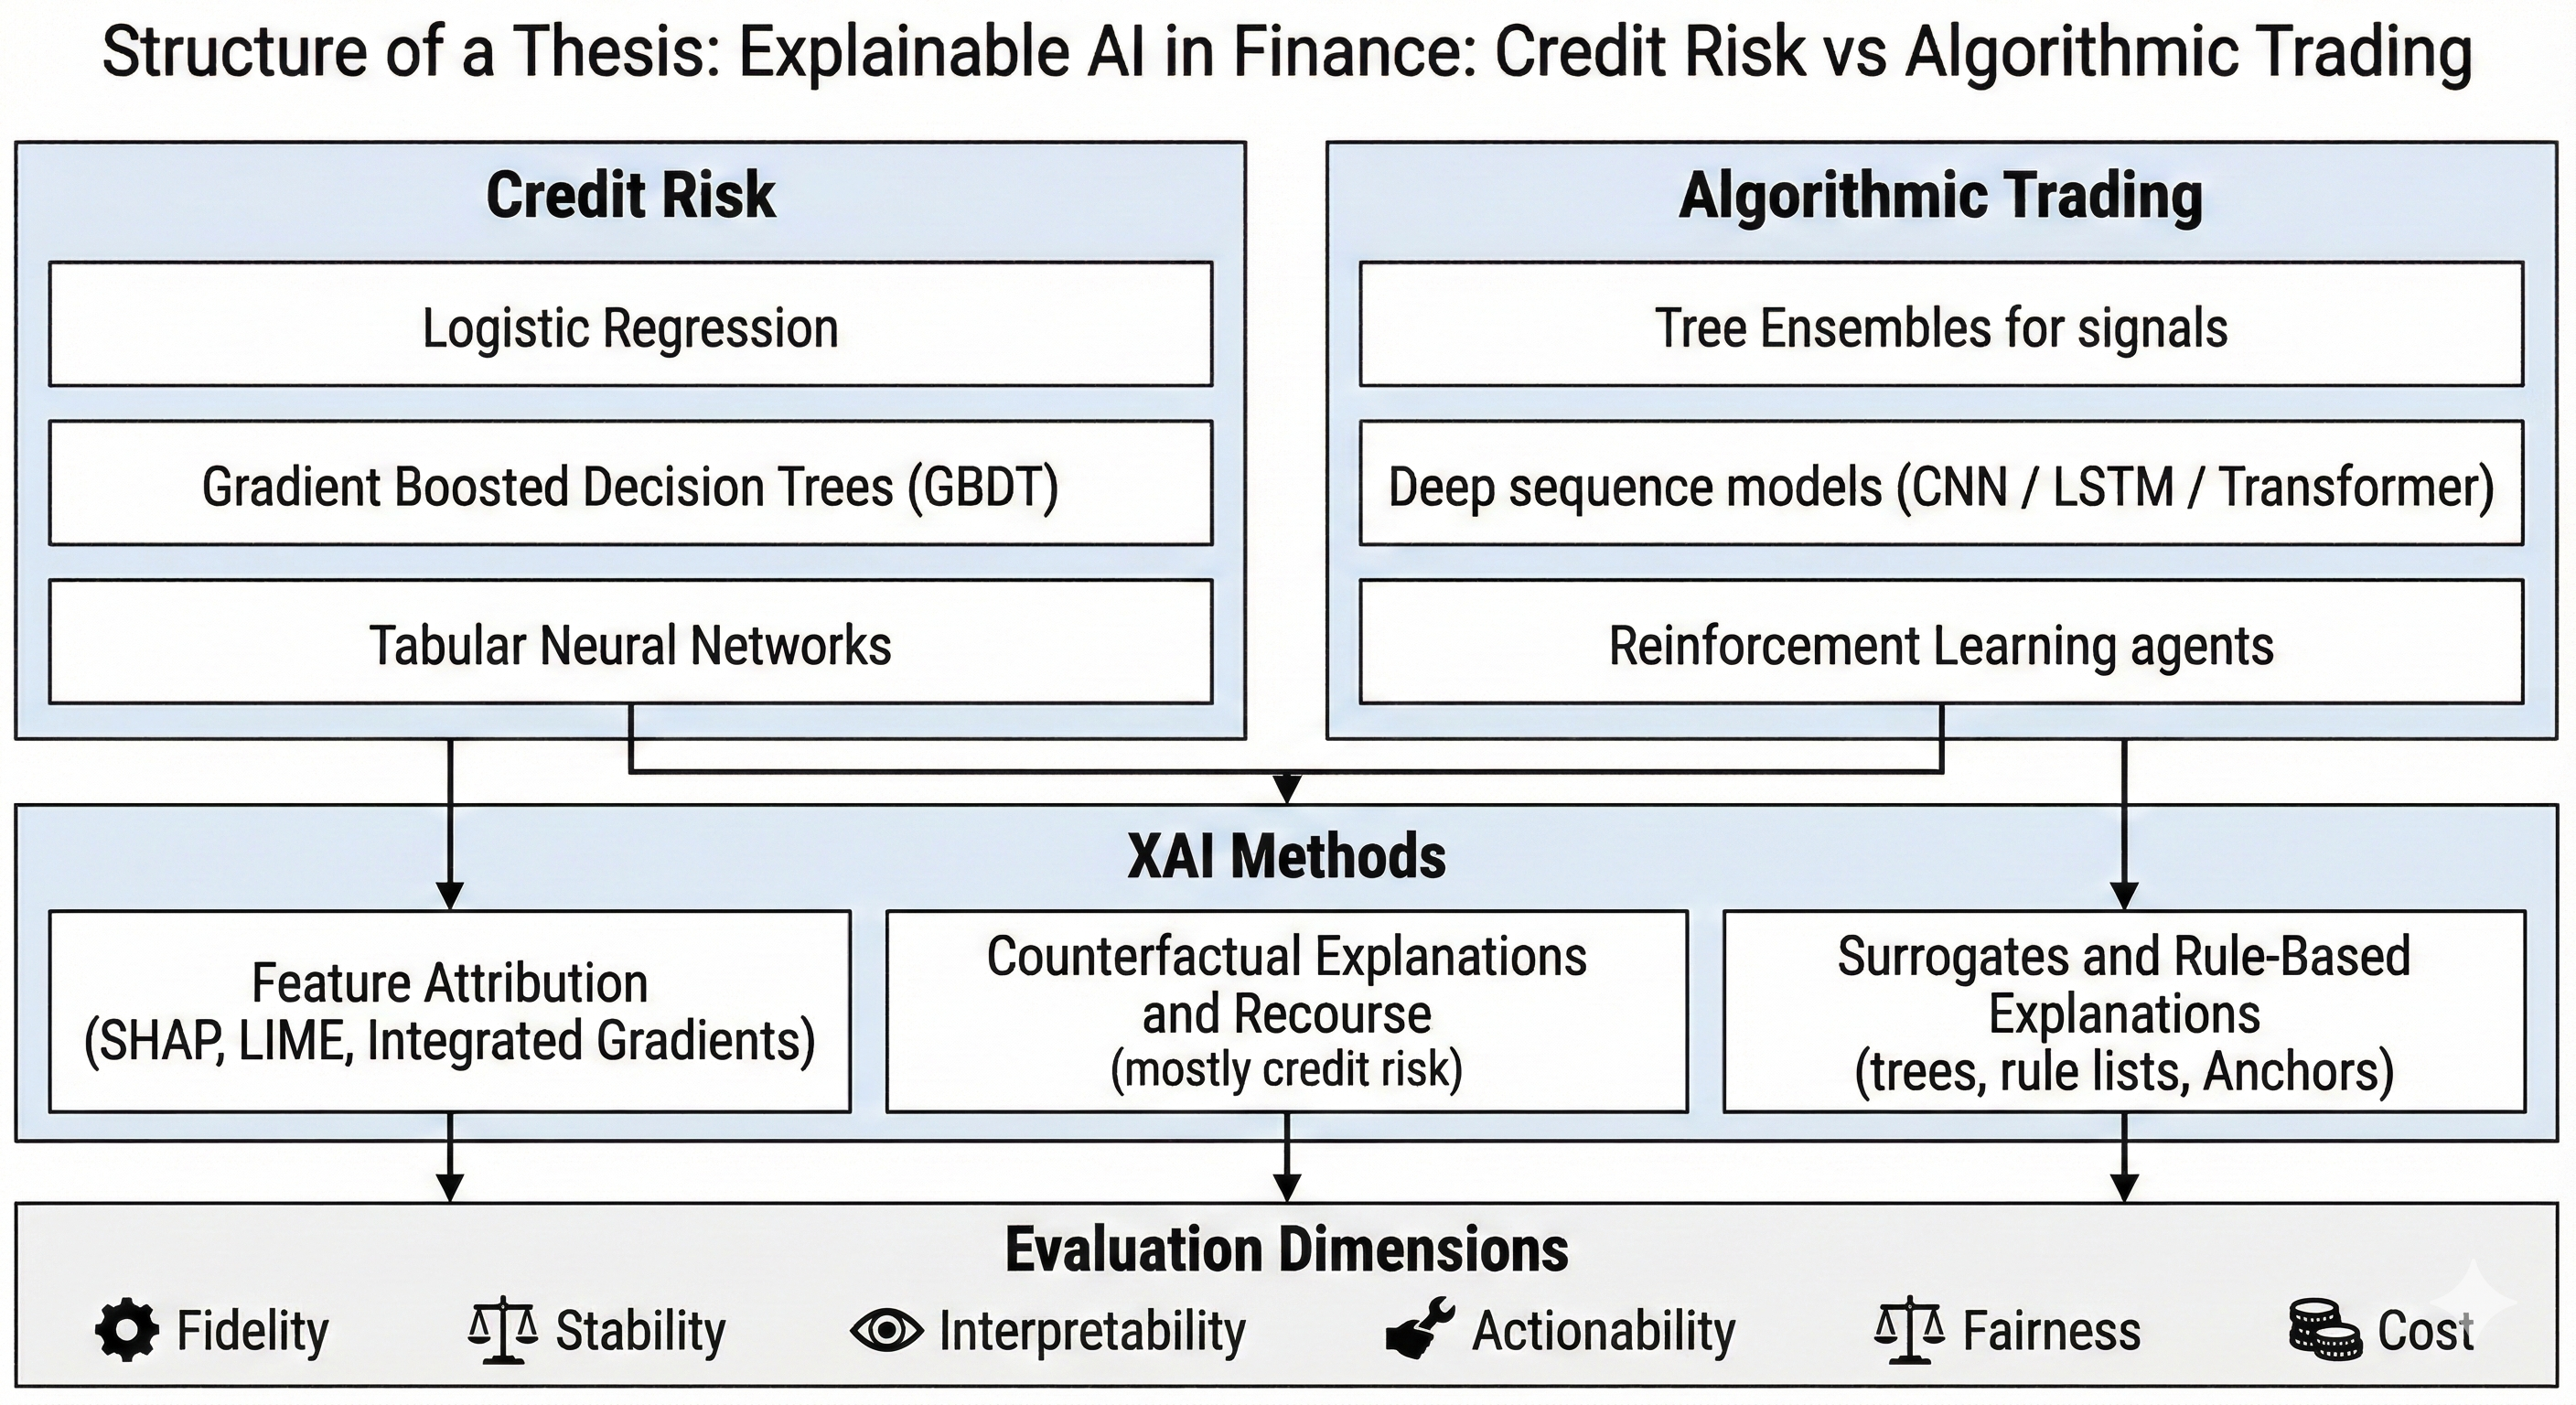
\includegraphics[width=1\textwidth]{imgs/Structure.png}
  \caption[Thesis Structure]{\textbf{Thesis Structure.}}
  \label{fig: structure}
\end{figure}

% =========================
% Chapter 2: Credit Risk and Lending Decisions
% =========================
\chapter{Credit Risk and Lending Decisions}
\label{chap:credit-risk}

Credit risk is the risk that a borrower will be unable to repay a debt obligation. It is the dominant risk faced by banks, mortgage lenders, leasing firms and credit card issuers, and largely determines how much credit an economy can safely extend, and at what price. Poor or inadequate management of credit risk can create substantial losses, as illustrated by the 2008 global financial crisis.

Regulatory and internal risk frameworks usually describe credit risk in terms of three key variables: the probability of default (PD), the loss given default (LGD) and the exposure at default (EAD), that is, the outstanding amount plus any expected further drawings at the time of default. For a single exposure, the expected loss (EL) over a given horizon is
\begin{equation}
  \mathrm{EL} = \mathrm{PD} \times \mathrm{LGD} \times \mathrm{EAD}.
  \label{eq:el-pd-lgd-ead}
\end{equation}
The product structure in \eqref{eq:el-pd-lgd-ead} makes explicit that expected loss increases both with the likelihood of default (PD) and with the severity (LGD) and size (EAD) of the position. This quantity is required to price loans and to create provisions and capital for the various stages of the lending process: origination, ongoing monitoring and workout.

Recent surveys report that around 44\% of XAI-in-finance studies focus on credit-related tasks (credit scoring and credit risk assessment), ahead of risk management and trading.\cite{XAiLiteratureReview2024}. Beyond predictive accuracy, AI and XAI are used to explain credit risk assessments so that stakeholders can understand why a credit decision was reached and which factors drove the predicted default risk, supporting both economic objectives (risk management and pricing) and legal/ethical requirements (transparency, non-discrimination and rights to explanation) \cite{XAiFinancialRisk,XAiFinanceReview2025}.

Credit risk is embedded in the entire lending cycle. Creditors must decide whether to grant credit, how much, at what interest rate, and under which repayment terms and collateral arrangements. They then monitor the borrower’s situation (continuous behavioural monitoring for retail credit, early-warning triggers in SME and corporate credit) and may adjust limits or increase reserves to protect against future defaults. When default occurs, lenders must quantify losses and estimate recoveries from pledged collateral.

\section{Financial Problem Definition}
\label{sec:credit-problem}

\subsection{Credit Scoring and Default Prediction}
\label{subsec:credit-risk-lending}

Credit scoring models translate information about borrower characteristics and contract terms into an assessment of default risk. In practice, they produce either a binary decision (good/bad, accepted/rejected) or a quantitative measure of default risk over a given horizon.

Formally, let $x \in \mathbb{R}^p$ denote an input vector representing borrower characteristics (e.g.\ income, employment, debt, past payment history, collateral) and contract terms (e.g.\ loan amount, maturity, interest rate, product type). A credit scoring model is a function
\begin{equation}
  f : \mathbb{R}^p \to [0,1]
  \label{eq:credit-score-function}
\end{equation}
where $f(x)$ is interpreted as the predicted probability that the borrower will default over the horizon of interest. To obtain a binary lending decision, institutions typically apply a threshold $\tau \in (0,1)$ to the score:
\begin{equation}
  \hat{y}(x) = 
  \begin{cases}
    1, & \text{if } f(x) \ge \tau,\\[4pt]
    0, & \text{if } f(x) < \tau,
  \end{cases}
  \label{eq:credit-decision-rule}
\end{equation}
where, depending on convention, $\hat{y}(x) = 1$ may denote “reject” (high risk) and $\hat{y}(x) = 0$ “accept” (low risk), or vice versa. More complex policies with multiple bands (automatic acceptance, manual review, automatic rejection) can still be expressed as functions of $f(x)$.

Automated scoring models reduce the time required to evaluate loan requests, free loan officer resources to focus on borderline or complex cases, enforce more consistent treatment of similar applications and allow a large number of predictive variables (behavioural, transactional, alternative data) to be incorporated into a single decision rule. Empirical work shows that machine learning techniques applied to consumer credit portfolios can reduce both Type I errors (approving loans that later default) and Type II errors (rejecting borrowers who would have repaid), improving risk-adjusted profitability and capital efficiency \cite{XAiCreditAssessment2022,XAiCreditScoring}.

Data characteristics differ across segments, although the main model families are shared. Retail consumer credit (credit cards, personal loans, vehicle financing, home equity lines) typically involves large, relatively homogeneous portfolios with many borrowers and a moderate set of static and behavioural features. SME lending adds richer balance sheet, accounting and relationship information but has fewer firms per segment and more noisy or missing data. Corporate and project finance deal with fewer, larger and more idiosyncratic exposures, with contractual covenants, industry and firm-specific variables and stronger dependence on macroeconomic conditions. Across these fields, logistic regression, scorecards and tree-based ensembles (gradient boosting) dominate; differences lie mainly in data structure, quality and granularity rather than in completely distinct modelling paradigms \cite{XAiLiteratureReview2024,XAiCreditScoring}.

Modern credit scoring datasets are often large, high-dimensional, imbalanced and heterogeneous. Retail explainable-credit-scoring studies frequently use datasets such as FICO HELOC or LendingClub consumer loans, with tens of thousands to millions of observations and tens to hundreds of numeric, ordinal and categorical variables \cite{XAiCreditScoring}. Default events are typically rare, creating challenges for estimation and evaluation. These data characteristics motivate complex machine learning models but also make it more difficult to understand why a specific borrower is classified as high or low risk.

Default prediction also plays a role beyond origination. Stress tests and macro–micro simulation frameworks require models that map macroeconomic scenarios and borrower characteristics to loan-level PDs. Machine learning models can capture nonlinear relationships between macro variables (GDP, unemployment, interest rates) and borrower-level features, allowing for more granular views of extreme losses. Explainability techniques are then used to determine which risk drivers dominate each segment and how their importance shifts across macro scenarios, which is crucial for understanding model behaviour in stressed but plausible conditions \cite{XAiDefaultRisk2019,XAiFinancialRisk}.

\section{AI Models Used}
\label{sec:credit-ai-models}

\subsection{Inference Models}
\label{sec:inference-models}

In this section, we discuss how the main model families for credit scoring function, as this provides the necessary background for understanding how XAI methods are applied to these models in subsequent sections.

\subsubsection{Logistic Regression}

As discussed in Section~\ref{subsec:statistical-to-ml}, the most widely employed baseline model for credit scoring is logistic regression \cite{XAiCreditRisk2020,XAiCreditAssessment2022}. Given a borrower \(n\) with feature vector
\[
  x_n = (x_{n1}, \dots, x_{nJ}),
\]
logistic regression models the log-odds of default as a linear function of the inputs,
\begin{equation}
  \log \frac{p_n}{1 - p_n}
  = \beta_0 + \sum_{j=1}^{J} \beta_j\,x_{nj},
  \label{eq:logit-credit}
\end{equation}
where \(p_n = \Pr(y_n = 1 \mid x_n)\) is the probability that borrower \(n\) defaults over a given horizon, \(\beta_0\) is the intercept and \(\beta_j\) are the regression coefficients. Inverting the logit link in \eqref{eq:logit-credit} gives the default probability
\begin{equation}
  p_n
  = \left(1 + \exp\left(-\beta_0 - \sum_{j=1}^{J} \beta_j\,x_{nj}\right)\right)^{-1}.
  \label{eq:logistic-prob}
\end{equation}

The coefficients \(\beta = (\beta_0,\dots,\beta_J)\) are typically estimated by maximising the Bernoulli log-likelihood
\begin{equation}
  \ell(\beta)
  = \sum_{n=1}^N \left[
    y_n \log p_n + (1 - y_n)\log(1 - p_n)
  \right],
  \label{eq:logit-loglik}
\end{equation}
often with \(L_1\) or \(L_2\) penalisation to stabilise the model and limit overfitting \cite{InterpretableModels}. The estimated probabilities \(p_n\) are then calibrated and used as PDs in downstream risk and capital calculations.

\begin{figure}[htbp]
  \centering
  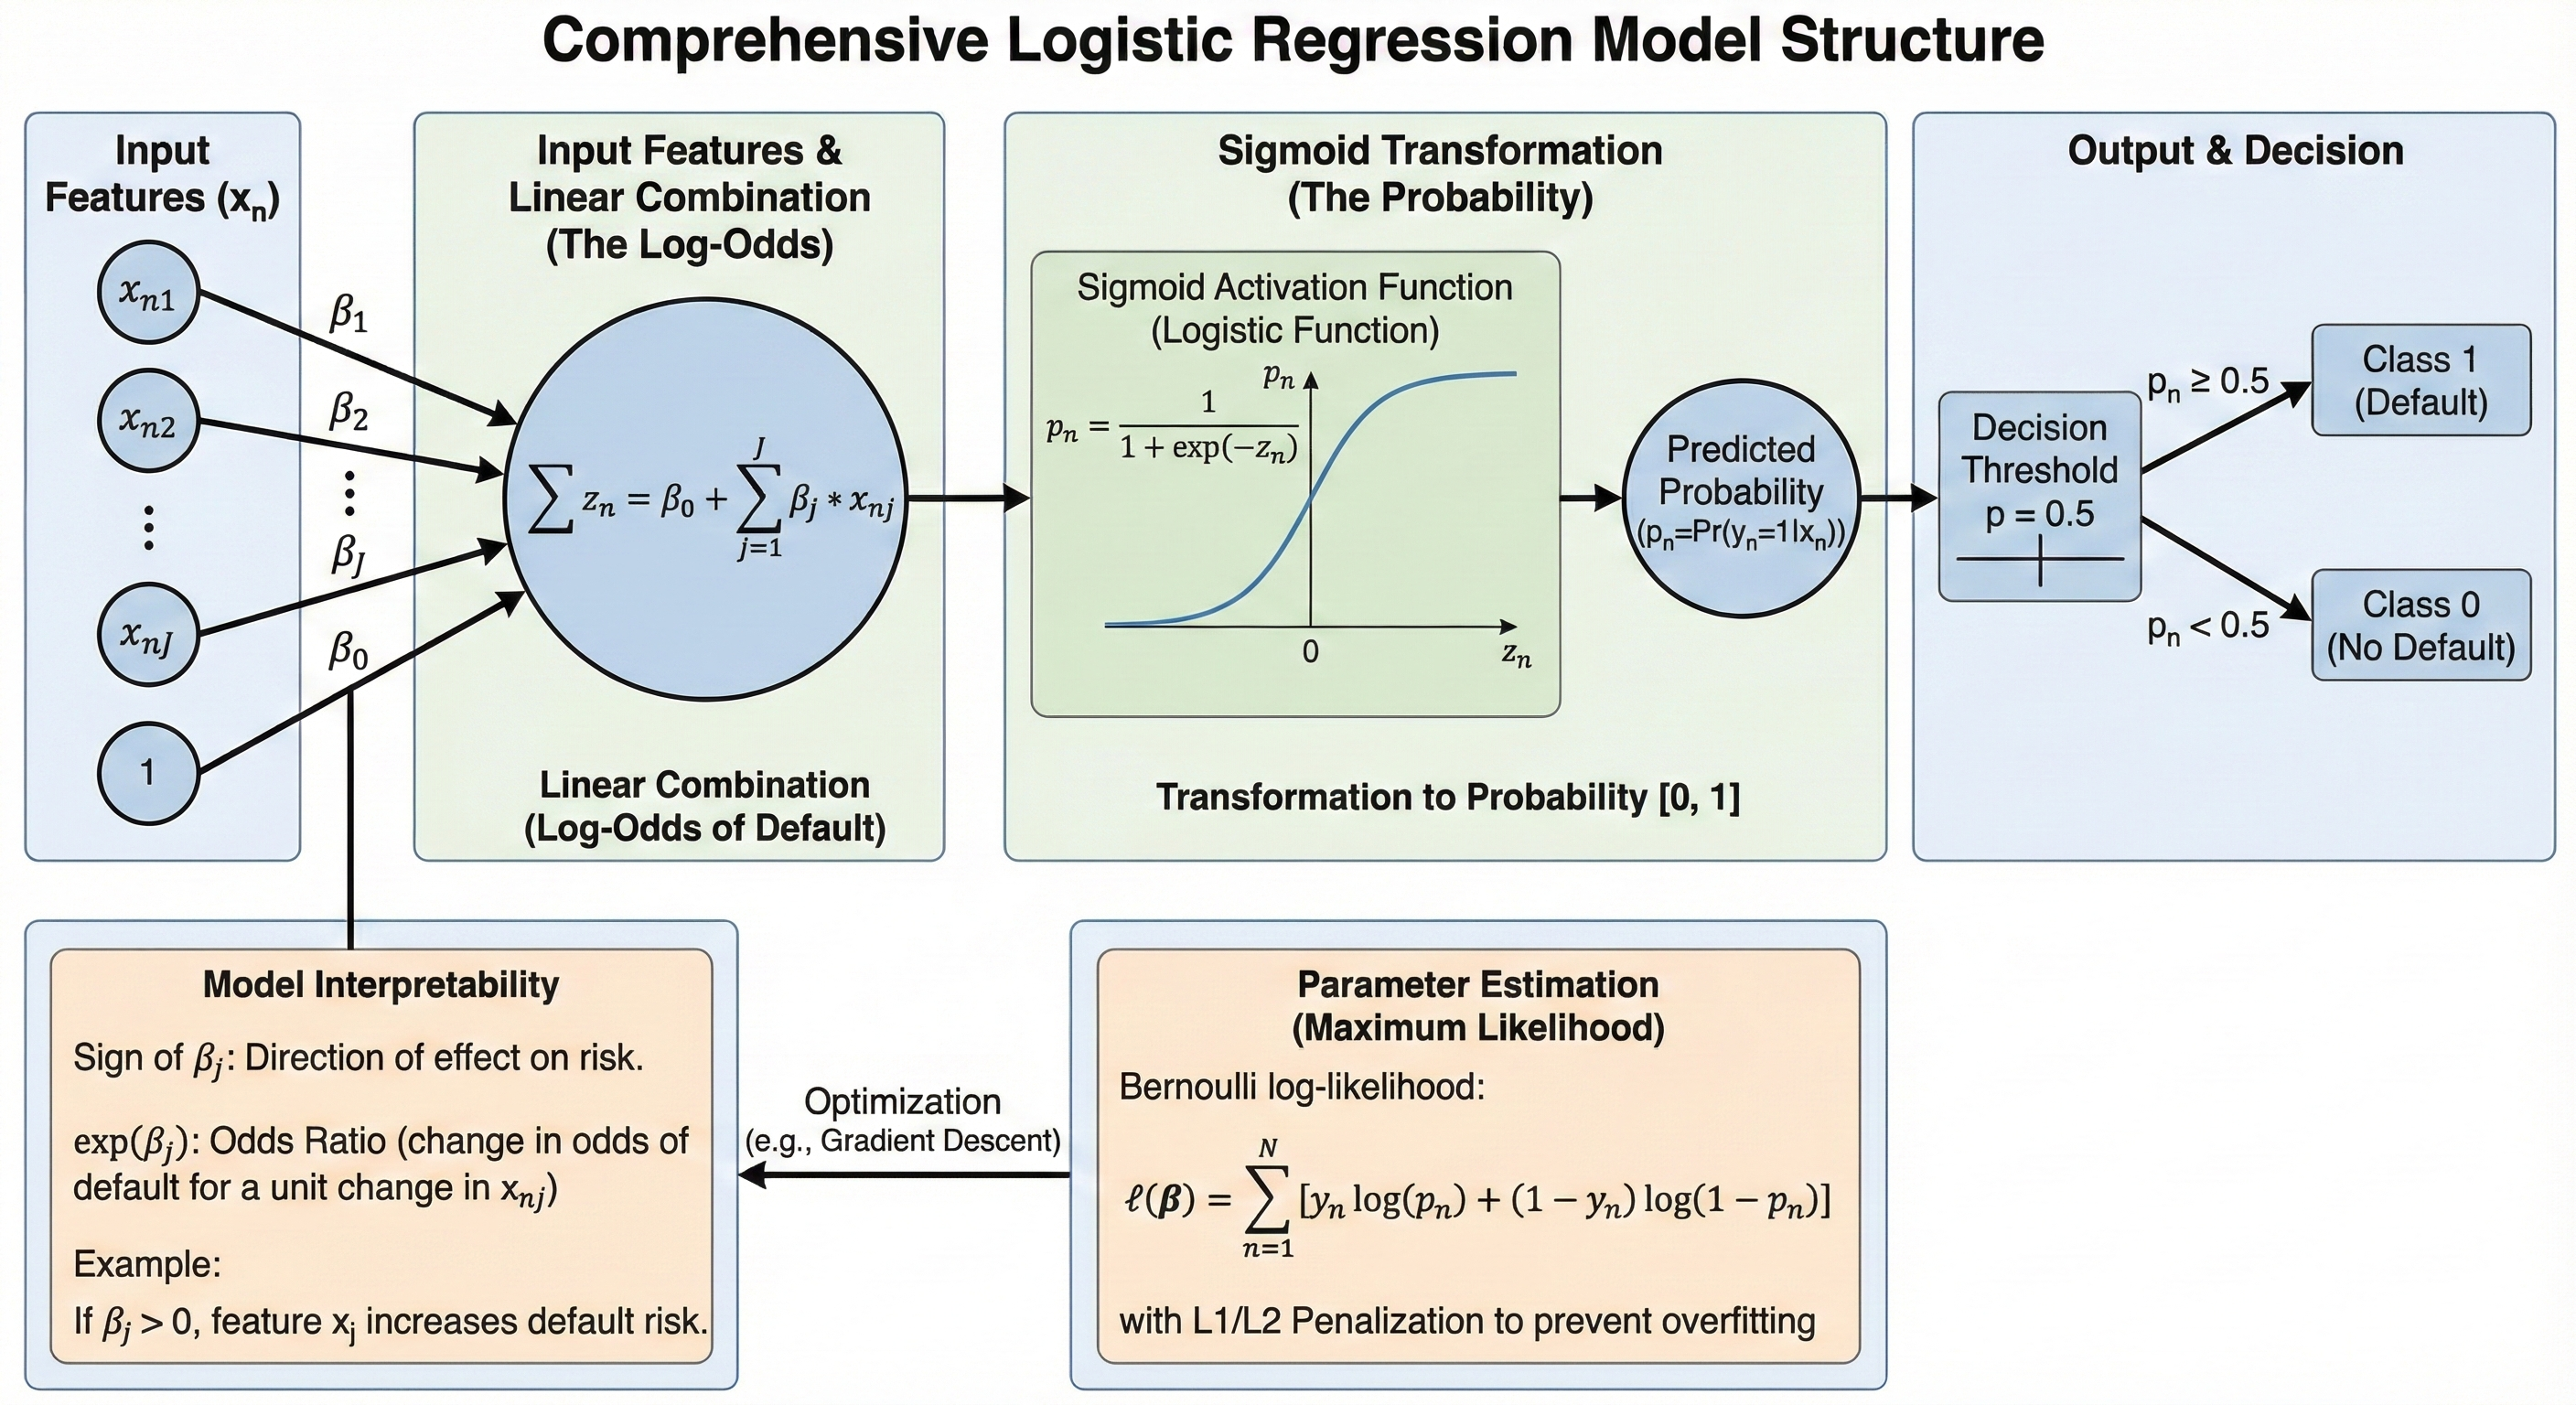
\includegraphics[width=1\textwidth]{imgs/LR.png}
  \caption[Logistic Regression in Credit Risk]{\textbf{Logistic Regression in Credit Risk.}}
  \label{fig:LR}
\end{figure}


Logistic regression remains attractive in credit risk for several reasons. First, its parameters admit a direct interpretation: in \eqref{eq:logit-credit}, the sign of \(\beta_j\) indicates whether feature \(x_j\) increases or decreases default risk and \(\exp(\beta_j)\) can be interpreted as an odds ratio. Secondly, the linear log-odds model in \eqref{eq:logit-credit} can be seen as a formal counterpart of traditional scorecard systems, where point scores are assigned to different levels of each feature and then summed. Thirdly, logistic regression is easy to fit, relatively robust for moderately sized samples and has an extensive history of use within the banking sector in relation to internal ratings-based approaches. These factors make logistic regression one of the most common benchmarks against which more complex machine learning models are compared \cite{XAiCreditRisk2020,XAiCreditAssessment2022}.

Additionally, due to its inherent simplicity and interpretability, logistic regression is used as the canonical example in Section~\ref{subsec:intrinsic-posthoc}, and it provides a baseline level of transparency that helps to meet the fairness, bias and documentation requirements listed in Section~\ref{subsec:fairness-bias} prior to the transition of the portfolio to the post-hoc methods of Section~\ref{subsec:feature-attribution}. However, logistic regression cannot easily capture non-linear relationships and complex interactions between variables. Credit risk relationships typically exhibit threshold effects, saturation, structural changes and non-constant variance as they relate to both the combination of application data and behavioural or transactional data \cite{XAiLiteratureReview2024,InterpretableModels}.

\subsubsection{Gradient Boosting Decision Trees}

To address these limitations while maintaining the tabular format of credit data, recent literature reviews of credit scoring models suggest that many practitioners now apply tree-based ensemble methodologies, specifically gradient boosting decision trees (GBDT) such as XGBoost and LightGBM \cite{XAiLiteratureReview2024,XAiFinanceReview2025}. Gradient boosting decision trees build an additive model of decision trees,
\begin{equation}
  f(x) = \sum_{m=1}^{M} \gamma_m\,T_m(x),
  \label{eq:gbdt-credit}
\end{equation}
where each \(T_m\) is a decision tree and \(\gamma_m\) are weights learned by sequentially fitting new trees on the pseudo-residuals (negative gradients) of a chosen loss function. For binary classification, this is typically the logistic loss
\[
  L(y, f(x)) = \log\bigl(1 + \exp(-y f(x))\bigr), \quad y \in \{-1,+1\},
\]
so that each boosting step focuses on observations whose PD is currently misestimated. A learning rate controls the contribution of each tree and trades off bias and variance.

The empirical evidence in the literature consistently shows that gradient boosting decision trees often outperform logistic regression on imbalanced credit default datasets. Both XGBoost and LightGBM achieve significantly better area under the receiver operating characteristic curve (AUROC, see Section~\ref{subsec:evaluation_metrics}) and precision–recall metrics compared to benchmark logistic regression models across peer-to-peer lending and bank consumer loans. Here, the ROC curve plots the true positive rate (share of correctly identified defaulters) against the false positive rate (share of non-defaulters incorrectly flagged as defaulters) as the decision threshold varies; the AUROC is the area under this curve and can be interpreted as the probability that a randomly chosen defaulter receives a higher risk score than a randomly chosen non-defaulter (with \(0.5\) corresponding to random guessing and \(1\) to a perfect ranking).

Therefore, the high performance of gradient boosting has become the de facto standard for high-performance credit default prediction, while simultaneously increasing the need for explainable AI. While the coefficients of logistic regression can be easily understood via \eqref{eq:logit-credit} and \eqref{eq:logistic-prob}, tree-based ensembles of the form \eqref{eq:gbdt-credit} require additional explanation techniques such as SHAP and partial dependence plots to understand how individual input features contribute to the assessment of the probability of default. Section~\ref{subsec:feature-attribution} draws upon the model landscape discussed above to detail the application of SHAP, LIME and similar techniques to open up the ``black box'' of tree-based ensemble models and produce audit trails of reason codes, as required by the fairness and conduct principles outlined in Section~\ref{subsec:fairness-bias}. For example, \cite{XAiCreditAssessment2022} applied TreeSHAP to LightGBM scores in a Norwegian unsecured-loans deployment, providing ECOA-style reason codes such as ``High utilisation added 0.5\% to the PD, three recent delinquencies added 0.8\%, stable income subtracted 0.6\%.''

\begin{figure}[htbp]
  \centering
  \includegraphics[width=0.7\textwidth]{imgs/5.jpg}
  \caption[Gradient Boosting Decision Tree Architecture]{\textbf{Gradient Boosting Decision Tree Architecture.} The first tree is trained on the original training set and its prediction errors are computed. Those errors are then used to construct a new, reweighted training set for the second tree, so that this tree concentrates on the examples that were predicted poorly by the first one; the same procedure is repeated for all subsequent trees. In the lower part of the figure, the individual tree models are collected into an ensemble classifier: when test data are input, each tree produces a prediction and these predictions are aggregated to obtain the final output of the model.}
  \label{fig:gbdt}
\end{figure}


\subsubsection{Random Forests and Related Ensembles}

In addition to gradient boosting, other tree-based ensembles such as random forests have been widely used for credit scoring. Random forest models use multiple decision trees. Each decision tree is trained on a bootstrap sample of the dataset and a random subset of the features, which helps reduce the variance of the model and captures nonlinear relationships in the data. The random forest prediction for an input \(x\) can be written as
\begin{equation}
  f_{\mathrm{RF}}(x)
  = \frac{1}{K} \sum_{k=1}^{K} T_k(x),
  \label{eq:rf-credit}
\end{equation}
where \(T_k\) denotes the \(k\)-th tree and \(K\) is the number of trees in the forest. In probability-estimation settings such as PD modelling, each tree typically outputs a class probability and \(f_{\mathrm{RF}}(x)\) is their average.

\begin{figure}[htbp]
  \centering
  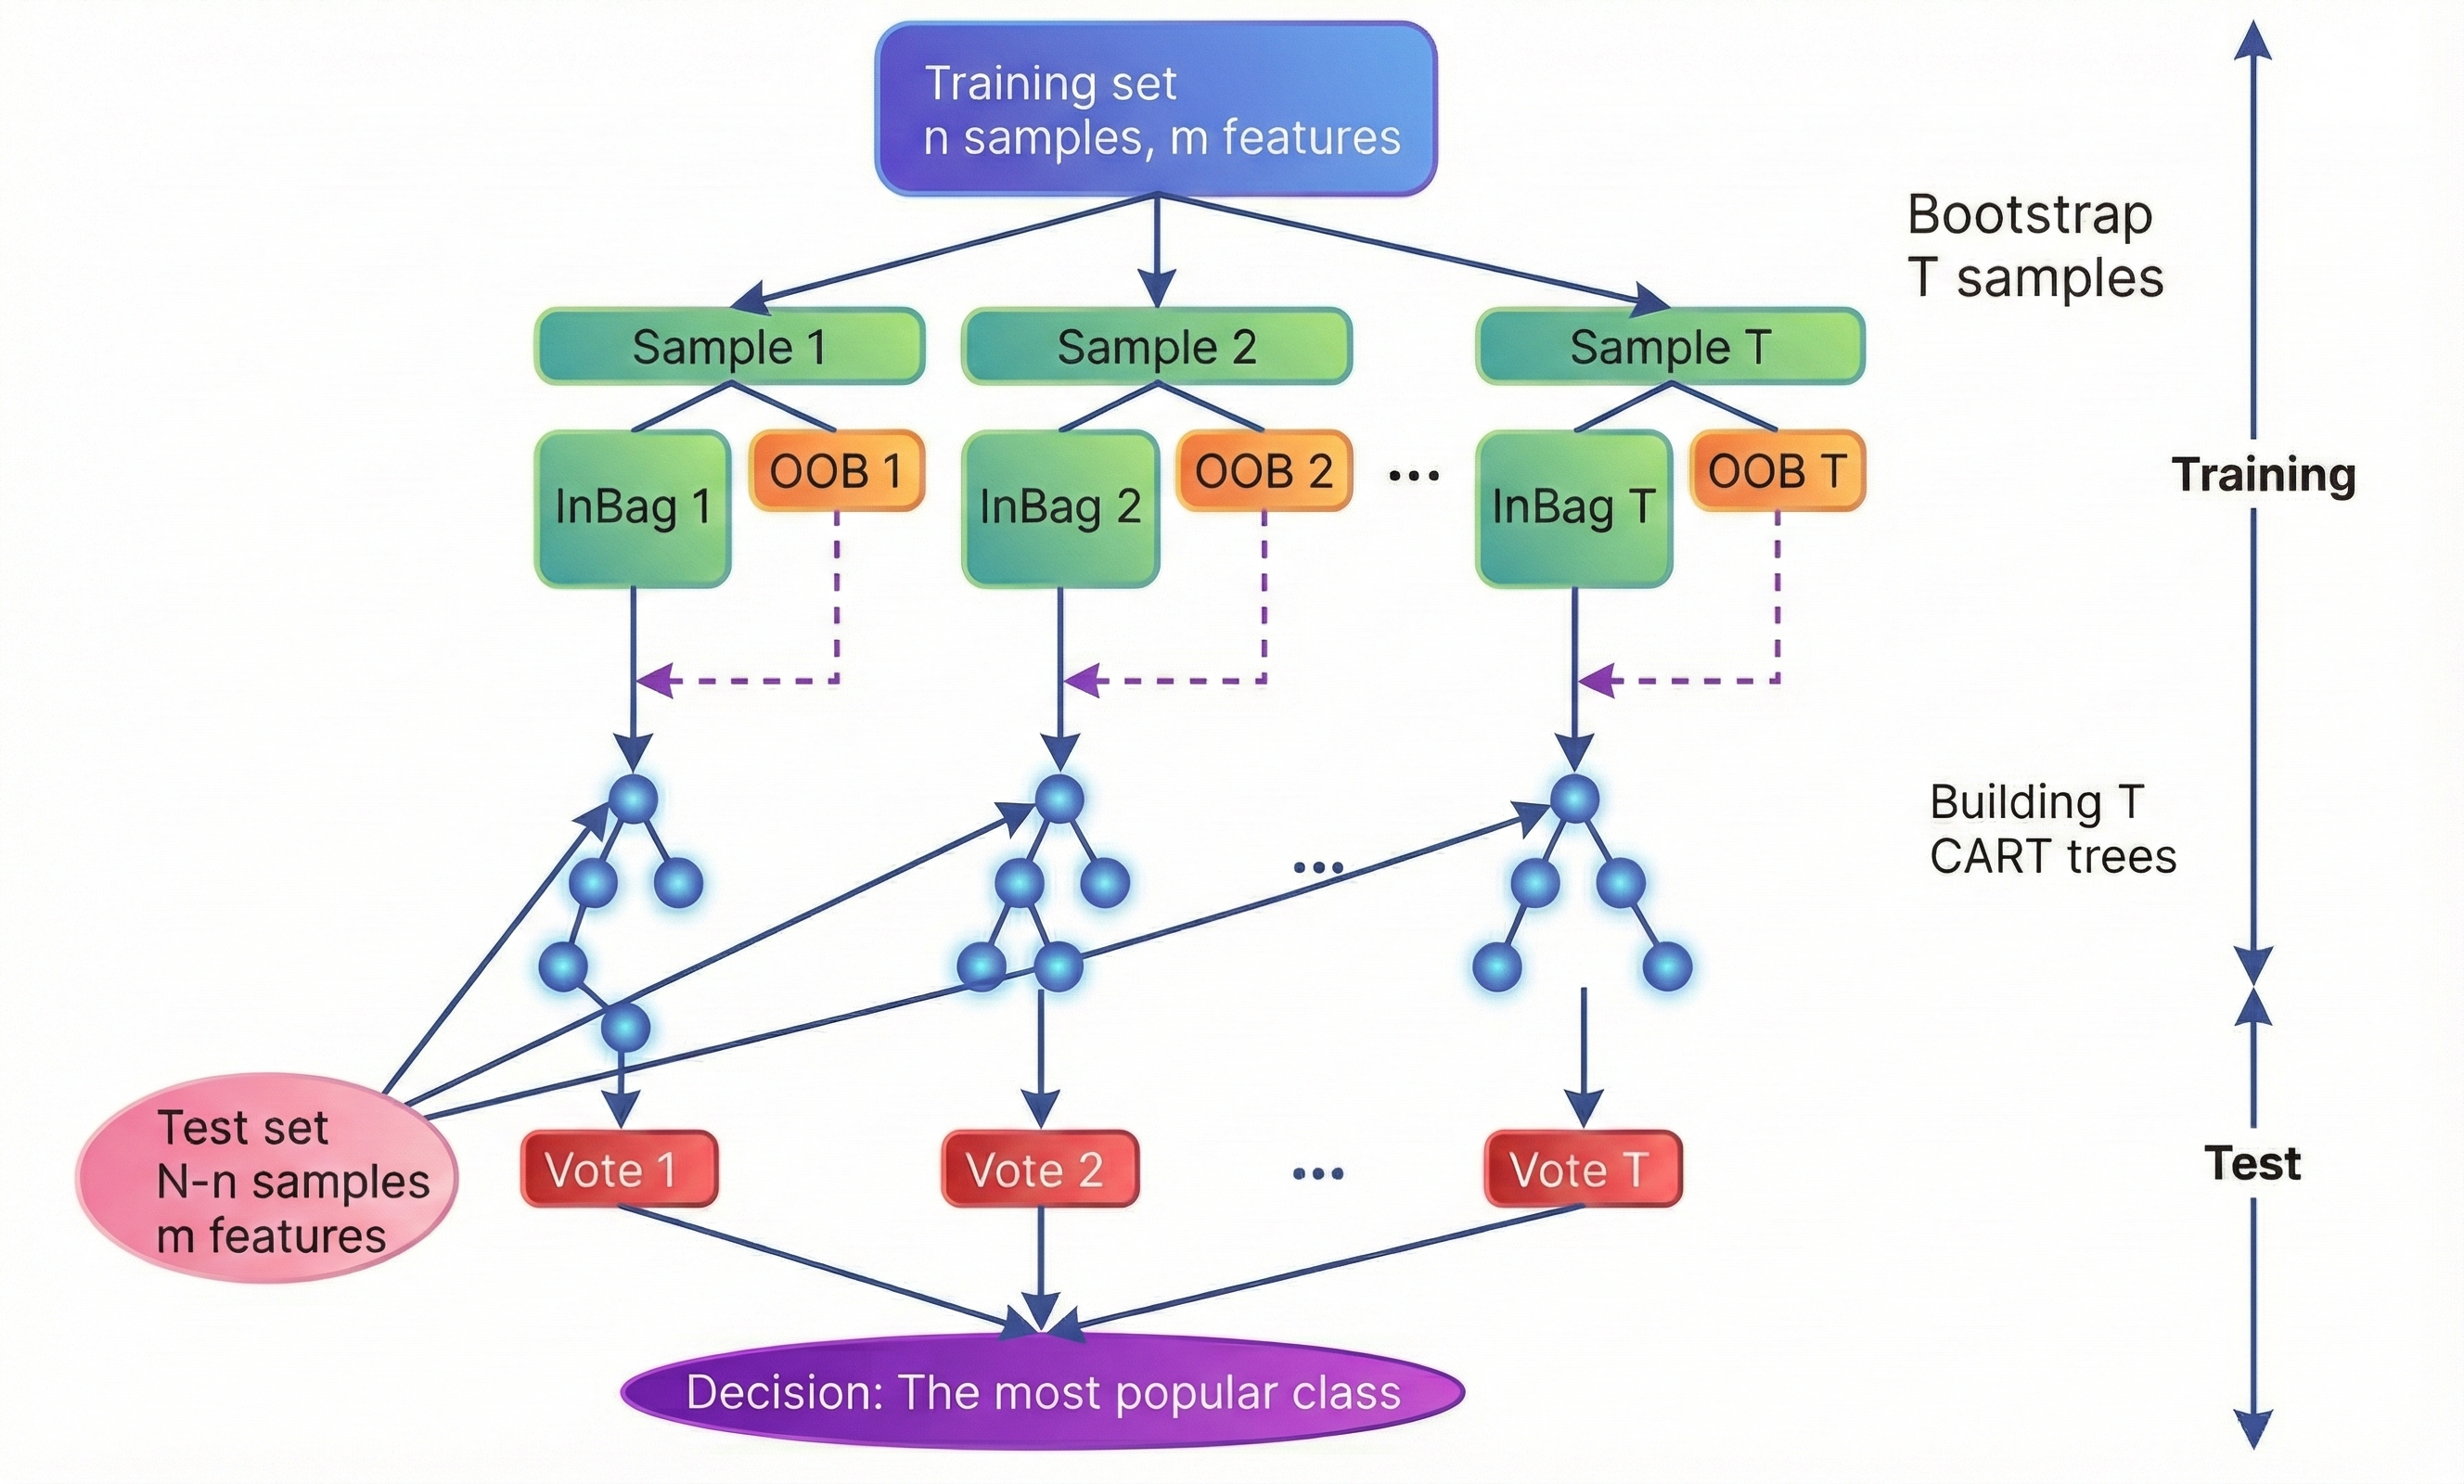
\includegraphics[width=0.7\textwidth]{imgs/6.png}
  \caption[Random Forest training and prediction]{\textbf{Random forest training and prediction.}
  From the original training set with \(n\) samples and \(m\) features, the algorithm draws
  \(T\) bootstrap samples. For each sample, the observations that are selected (in-bag) are
  used to train one decision tree, while the observations that are not selected (out-of-bag)
  can be used as an internal validation set. At test time, each tree receives the feature
  vector of a new observation and outputs a class prediction; the random forest aggregates
  these tree predictions by majority vote to obtain the final class.}
  \label{fig:RF}
\end{figure}

Random forest models have achieved state-of-the-art performance in several benchmark studies using datasets such as HELOC and LendingClub, surpassing the performance of shallow neural networks and logistic regression \cite{XAiCreditScoring,XAiLiteratureReview2024}. Due to the heterogeneity and mixed type of credit data, including the presence of numerical and categorical variables, missing values and nonlinear effects, models such as random forests and XGBoost require relatively little manual feature engineering compared to traditional linear models.

\subsubsection{Neural Networks and Sequential Architectures}

Deep neural networks have also been researched for credit scoring applications, primarily through fully connected feedforward networks (multilayer perceptrons). In general, these models define a parametrised mapping
\begin{equation}
  f_\theta : \mathbb{R}^p \to [0,1],
  \label{eq:dnn-credit}
\end{equation}
where \(\theta\) denotes the weights and biases across multiple layers and \(f_\theta(x)\) outputs an estimated probability of default (PD) for a feature vector \(x \in \mathbb{R}^p\).

For an \(L\)-layer feedforward network, the computation can be written in a compact way as
\begin{align}
  h^{(0)} &= x, \\
  h^{(\ell)} &= \sigma\!\bigl(W^{(\ell)} h^{(\ell-1)} + b^{(\ell)}\bigr), \quad \ell = 1,\dots,L, \\
  f_\theta(x) &= \sigma\!\bigl(w^\top h^{(L)} + b\bigr),
\end{align}
where \(h^{(\ell)}\) is the vector of activations at layer \(\ell\), \(W^{(\ell)}\) and \(b^{(\ell)}\) are layer-specific weights and biases, \(w\) and \(b\) parameterise the final output layer and \(\sigma\) is a non-linear activation function (e.g.\ ReLU in hidden layers, logistic in the output layer). Intuitively, each layer forms a weighted combination of the previous layer’s outputs and then applies a non-linearity, allowing the network to approximate non-linear decision boundaries in the original feature space.

The parameters \(\theta\) are typically learned by minimising the (possibly class-weighted) binary cross-entropy loss
\[
  \mathcal{L}(\theta)
  = - \sum_{n=1}^{N} \left[
  \alpha\, y_n \log f_\theta(x_n)
  + (1-y_n)\log\bigl(1 - f_\theta(x_n)\bigr)
  \right],
\]
where \(y_n \in \{0,1\}\) indicates whether borrower \(n\) defaulted, and \(\alpha > 1\) can up-weight the minority (default) class in imbalanced datasets. Regularisation terms (e.g.\ \(L_1\)/\(L_2\) penalties or dropout) are often added to control overfitting.

\begin{figure}[htbp]
  \centering
  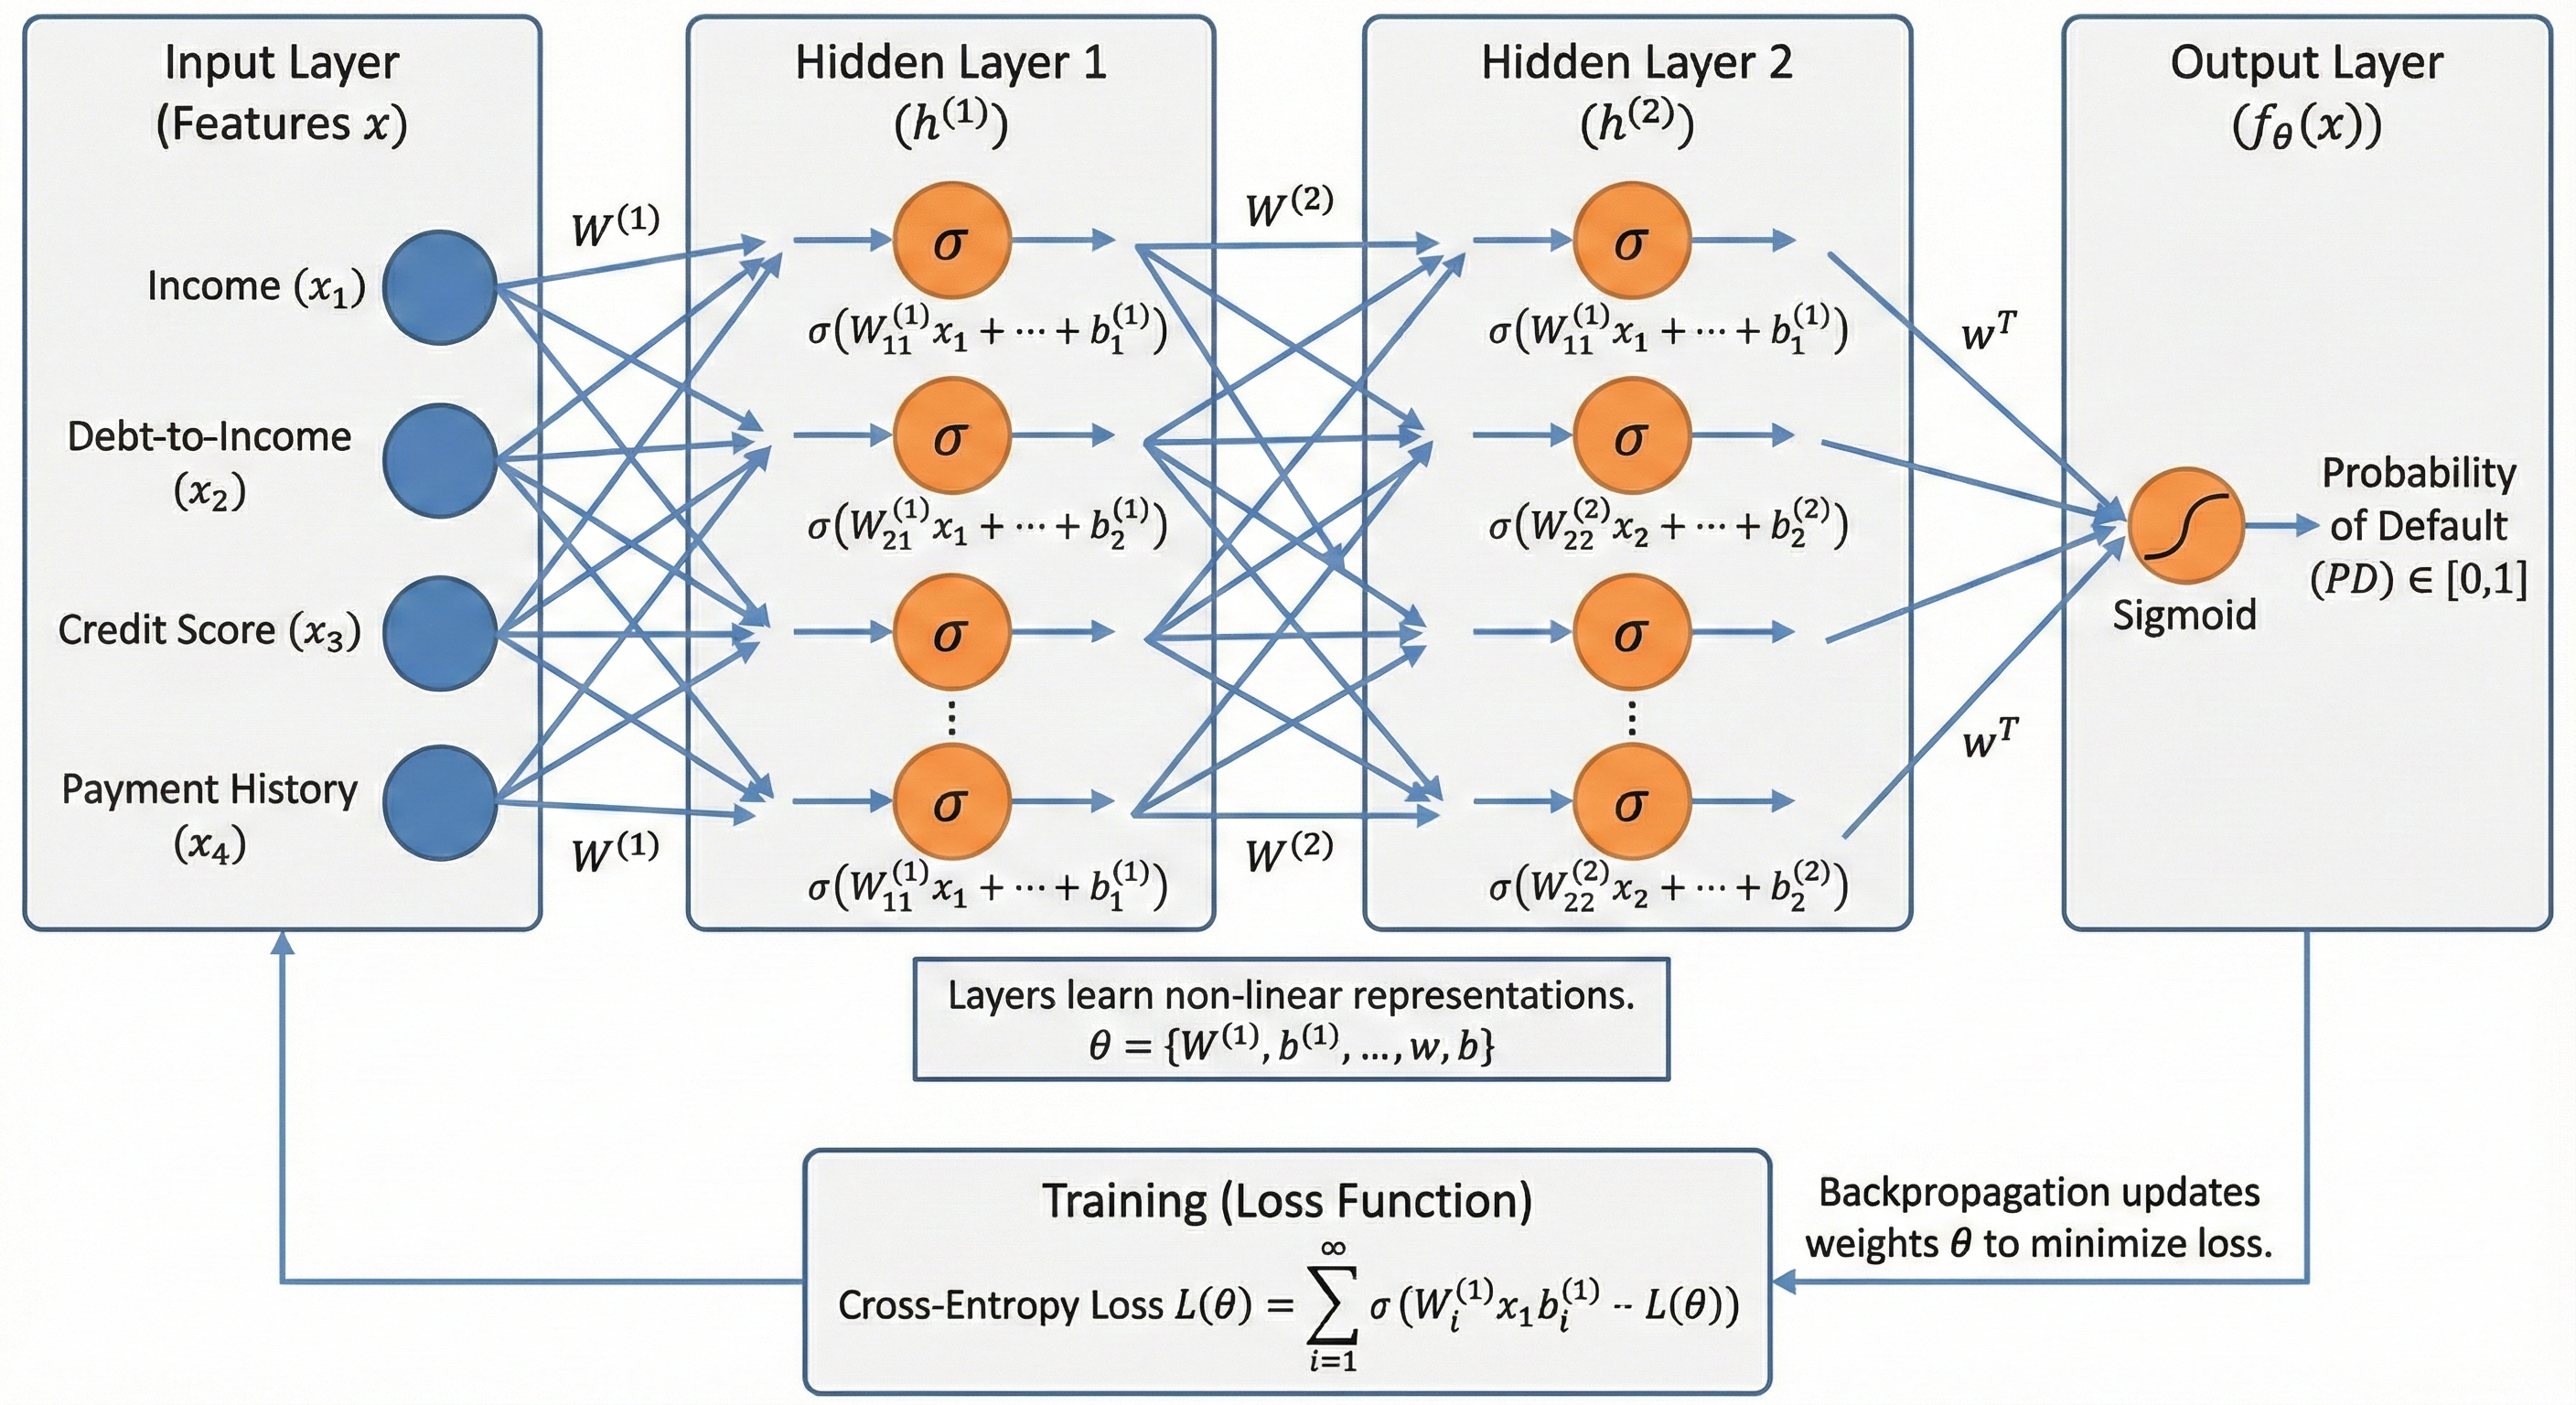
\includegraphics[width=1\textwidth]{imgs/NN.png}
  \caption[Neural Network]{\textbf{Neural Network Architecture.} A multilayer perceptron maps a vector of borrower features through successive linear transformations and non-linear activations to produce a probability of default in \([0,1]\).}
  \label{fig:NN}
\end{figure}

While a multilayer perceptron of the form \eqref{eq:dnn-credit} can, in principle, approximate complex decision boundaries in high-dimensional spaces and therefore seems an ideal choice for large credit datasets, in practice empirical results have been mixed. A study using an explainable credit scoring model initially employed a deep neural network as its primary classifier; however, it was ultimately replaced by a tree-based model because experiments showed that the DNN either underperformed or overfit, classifying nearly every instance into the majority class in highly imbalanced datasets \cite{XAiCreditScoring}. This result is consistent with broader evidence that, for structured tabular data with moderate numbers of features, tree ensemble methods often exceed feedforward networks in both performance and robustness \cite{InterpretableModels,XAiLiteratureReview2024}.

Neural networks tend to provide clearer advantages when the input extends beyond static application features. When behavioural information that changes over time (e.g.\ monthly account balances, transaction flows or payment history) is incorporated into credit scoring models, sequence models and hybrid architectures become applicable. A simple recurrent neural network (RNN) can, for example, process a sequence of \(T\) monthly behavioural vectors \(b_1,\dots,b_T\) via
\begin{align}
  h_0 &= 0, \\
  h_t &= \phi\!\bigl(W_h h_{t-1} + W_x b_t + c\bigr), \quad t = 1,\dots,T, \\
  \mathrm{PD} &= \sigma\!\bigl(w^\top h_T + b\bigr),
\end{align}
where \(h_t\) summarises the borrower’s behaviour up to month \(t\), \(\phi\) is a non-linear activation and \(h_T\) is the final latent summary used to predict the probability of default. In practice, this hidden state \(h_T\) is often concatenated with static application features and either fed into a final dense layer or into a tree-based model such as LightGBM. More sophisticated recurrent architectures (LSTMs, GRUs) and temporal convolutional networks (TCNs) follow the same principle but can capture longer-range temporal dependencies and more complex patterns \cite{XAiTimeSeriesForecasting2024}.

Case studies such as \cite{XAiCreditAssessment2022} show how such hybrid models can still be explained with TreeSHAP or DeepSHAP, turning behavioural motifs (e.g.\ “three consecutive missed payments in the last quarter’’) into basis-point adjustments in PD and thus into concrete reason codes. 

\subsection{Fairness, Bias and Regulatory Requirements}
\label{subsec:fairness-bias}

Decisions made through credit scoring and lending have social and legal implications, since they affect households’ and firms’ access to credit and can either exacerbate or mitigate existing inequalities. Most jurisdictions therefore impose both prudential requirements (e.g.\ capital adequacy, sound risk management) and conduct requirements (e.g.\ non-discrimination, consumer protection, transparency) on credit institutions. In the European Union, the General Data Protection Regulation (GDPR) has been interpreted as granting data subjects a right to an explanation for meaningful automated decisions, while sector-specific regulation such as the Equal Credit Opportunity Act (ECOA) in the United States requires lenders to provide ``adverse action'' notices that state the main reasons for denying credit \cite{Counterfactual,XAiFinancialRisk}.

Fairness and bias issues arise even when protected attributes (e.g.\ gender, race, age) are excluded from the feature set. Non-protected variables may act as proxies due to correlation (e.g.\ postcode, employment sector, income history), and standard optimisation objectives such as accuracy or AUROC do not enforce equal error rates or calibration across groups. The opacity of complex models further complicates the task of determining whether adverse decisions arise from legitimate risk drivers or from historical biases and spurious correlations in the data \cite{InterpretableModels,XAiFinancialRisk}.

Explainable AI does not guarantee fairness, but it provides diagnostic tools to assess and document model behaviour. In credit scoring, feature-attribution and global explanation frameworks (e.g.\ SHAP-based analyses) can be used to check whether protected or proxy variables systematically drive decisions and whether the main risk drivers are economically plausible \cite{SHAP,XAiCreditAssessment2022,XAiCreditScoring}. Counterfactual explanations support individual recourse by indicating behavioural changes that would have flipped the outcome and by revealing when realistic recourse is unavailable \cite{Counterfactual}. Supervisory authorities have begun to incorporate such tools into explainability frameworks for default and mortgage models, while stressing that explanations must be interpreted cautiously in policy applications \cite{XAiDefaultRisk2019,XAiFinancialRisk}. 

\subsection{Feature Attribution (SHAP, LIME)}
\label{subsec:feature-attribution}

Feature attribution assigns portions of a model’s prediction to individual input features. In credit scoring, this corresponds to assigning “reason codes” to drivers such as high utilisation, recent delinquencies or low income, and quantifying their impact on the predicted PD. This section introduces the general framework, presents LIME and SHAP as widely used methods and summarises their application in credit risk.

\begin{figure}[htbp]
  \centering
  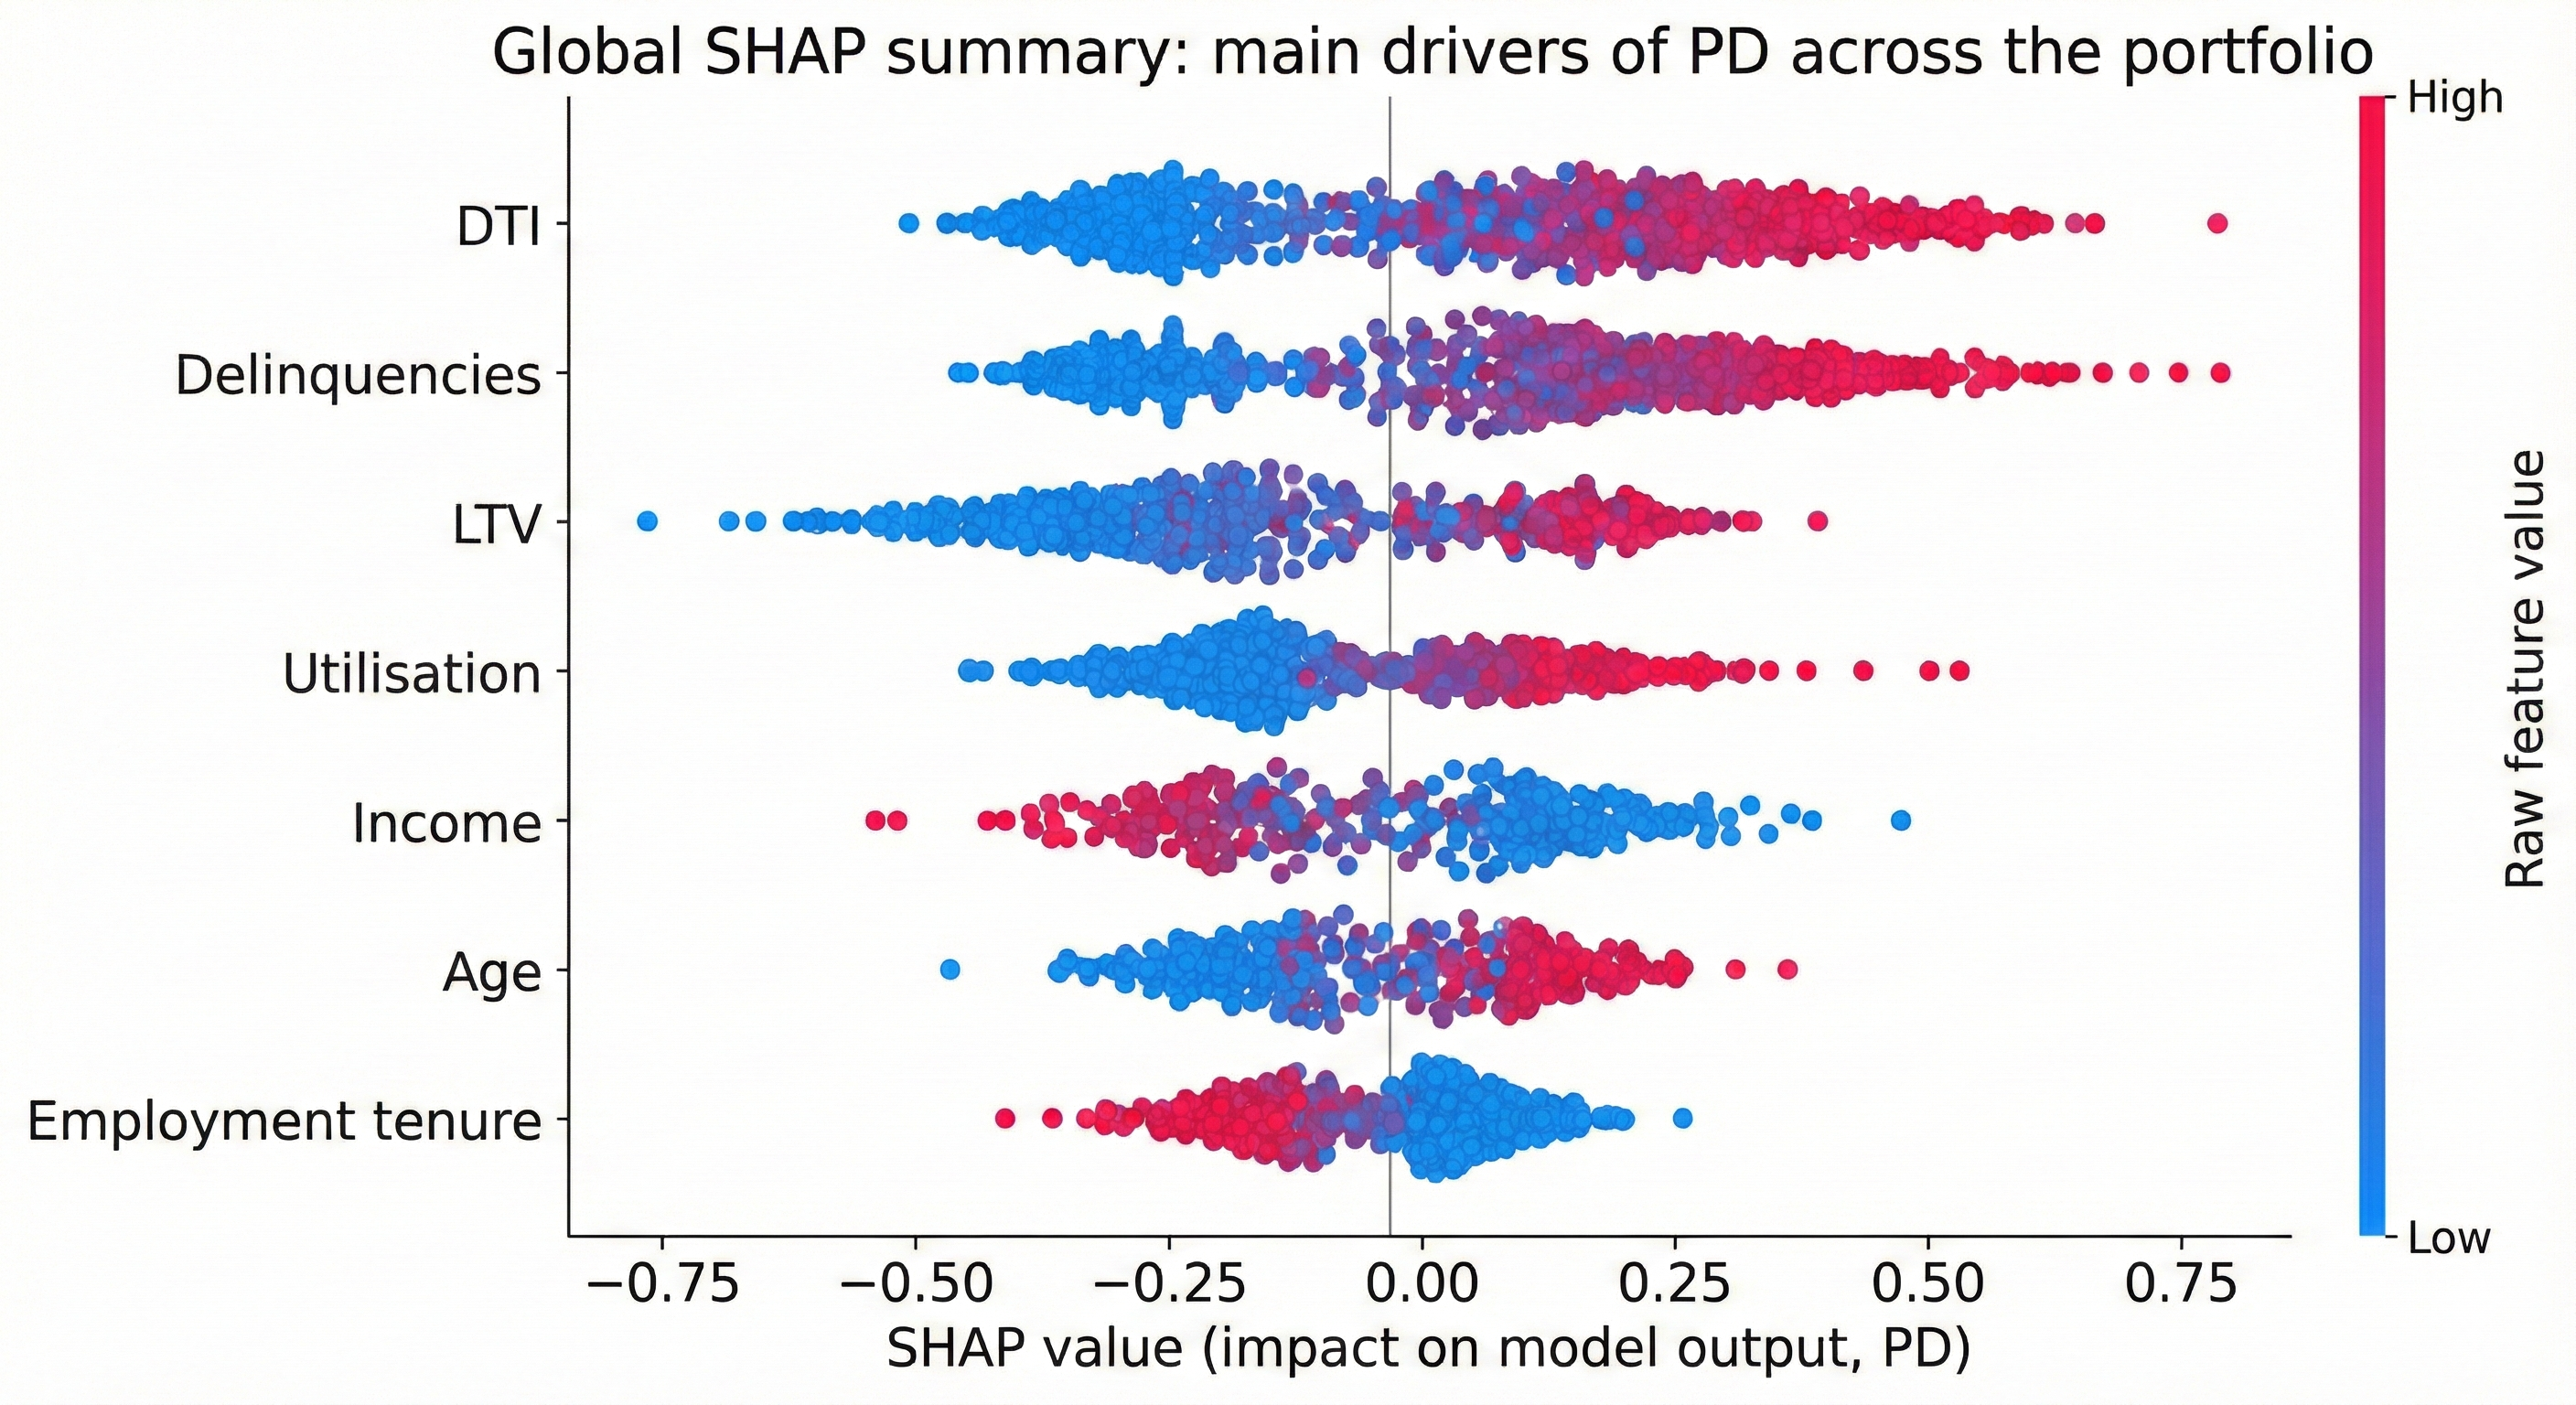
\includegraphics[width=0.8\textwidth]{imgs/GlobalSHAP.png}
  \caption[Global SHAP summary plot.]{\textbf{Global SHAP summary plot}}
  \label{fig:trading-global-shap}
\end{figure}

\subsubsection{Problem Setting and Notation}
\label{subsubsec:fa-notation}

Let \(x = (x_1,\dots,x_M)\) denote a feature vector for a single borrower and contract and let \(f(x)\) be a trained model that outputs a risk score, typically a predicted probability of default \(p(x) \in [0,1]\). A \emph{feature attribution} method associates to each prediction \(f(x)\) a vector
\[
\phi(x) = \bigl(\phi_1(x),\dots,\phi_M(x)\bigr)
\]
and optionally a baseline term \(\phi_0\), such that
\begin{equation}
  f(x) \approx \phi_0 + \sum_{j=1}^{M} \phi_j(x).
  \label{eq:fa-additive}
\end{equation}
The term \(\phi_j(x)\) is interpreted as the contribution of feature \(x_j\) to the prediction for this borrower, relative to the baseline \(\phi_0\). In classification problems, the decomposition can be done either on the probability scale (for example, percentage-point contributions to PD) or on a link scale such as log-odds, depending on the method.

A simple example fixes ideas. Suppose a bank uses a model \(f\) to estimate one-year PDs, with a portfolio-wide average PD of \(2\%\). For a specific mortgage application, the model outputs \(f(x) = 8\%\). A feature attribution method might produce
\[
\phi_0 = 2\%,\quad
\phi_{\text{LTV}}(x) = +3\%,\quad
\phi_{\text{arrears}}(x) = +4\%,\quad
\phi_{\text{income}}(x) = -1\%,
\]
so that Equation~\eqref{eq:fa-additive} holds exactly:
\[
f(x) = 2\% + 3\% + 4\% - 1\% = 8\%.
\]
For the credit officer, this reads as: high loan-to-value and existing arrears are the main drivers of risk, partially offset by high income.

Local attributions such as \(\phi(x)\) can be aggregated into \emph{global} importance measures by averaging over a portfolio. A common summary is the mean absolute attribution
\[
I_j = \frac{1}{N} \sum_{n=1}^{N} \bigl|\phi_j(x^{(n)})\bigr|,
\]
which quantifies how much feature \(j\) typically influences predictions across the dataset. In credit scoring studies, global importance rankings based on \(I_j\) are used to identify dominant risk drivers (for example, payment behaviour, utilisation, loan-to-income ratio) and to check that the model behaves consistently with domain knowledge \cite{XAiCreditRisk2020,XAiCreditAssessment2022,XAiCreditScoring}.

\subsubsection{LIME: Local Surrogate Explanations}
\label{subsubsec:lime-credit}

LIME (Local Interpretable Model-agnostic Explanations) approximates the behaviour of a complex model \(f\) in a small neighbourhood of a point \(x\) by fitting a simple, interpretable surrogate model \(g\) \cite{LIME}. In the tabular credit-risk setting, \(g\) is typically a sparse linear model, which can be interpreted similarly to a traditional scorecard.

LIME distinguishes between two spaces:
\begin{itemize}
  \item the \emph{original feature space} \(x \in \mathcal{X}\), where the model \(f\) operates (for example, credit bureau variables, behavioural scores, loan characteristics);
  \item an \emph{interpretable feature space} \(z \in \mathcal{Z}\), where explanations are expressed. For tabular data, \(z\) often coincides with \(x\), possibly after discretising continuous variables into bins (for example, LTV above or below 80\%).
\end{itemize}

Given a point \(x\) to be explained, LIME generates perturbed samples \(\{z'_k\}_{k=1}^{K}\) around the interpretable representation \(z\), computes model predictions \(f(z'_k)\) and fits a local surrogate \(g\) by solving
\begin{equation}
  \hat{g}
  = \arg\min_{g \in \mathcal{G}}
    \left[
      L\bigl(f, g, \pi_x\bigr)
      + \Omega(g)
    \right],
  \label{eq:lime-objective}
\end{equation}
where:
\begin{itemize}
  \item \(\mathcal{G}\) is the class of interpretable models, typically sparse linear models of the form
  \[
  g(z') = w_0 + \sum_{j=1}^{M} w_j z'_j;
  \]
  \item \(L(f,g,\pi_x)\) is a weighted loss (for example, weighted squared error) that penalises discrepancies between \(f(z'_k)\) and \(g(z'_k)\), with weights given by a locality kernel \(\pi_x(z'_k)\) that decays with the distance between \(z'\) and \(z\);
  \item \(\Omega(g)\) is a complexity penalty that favours sparse explanations, such as an \(\ell_1\)-type penalty on the number of non-zero coefficients.
\end{itemize}

\begin{figure}[htbp]
  \centering
  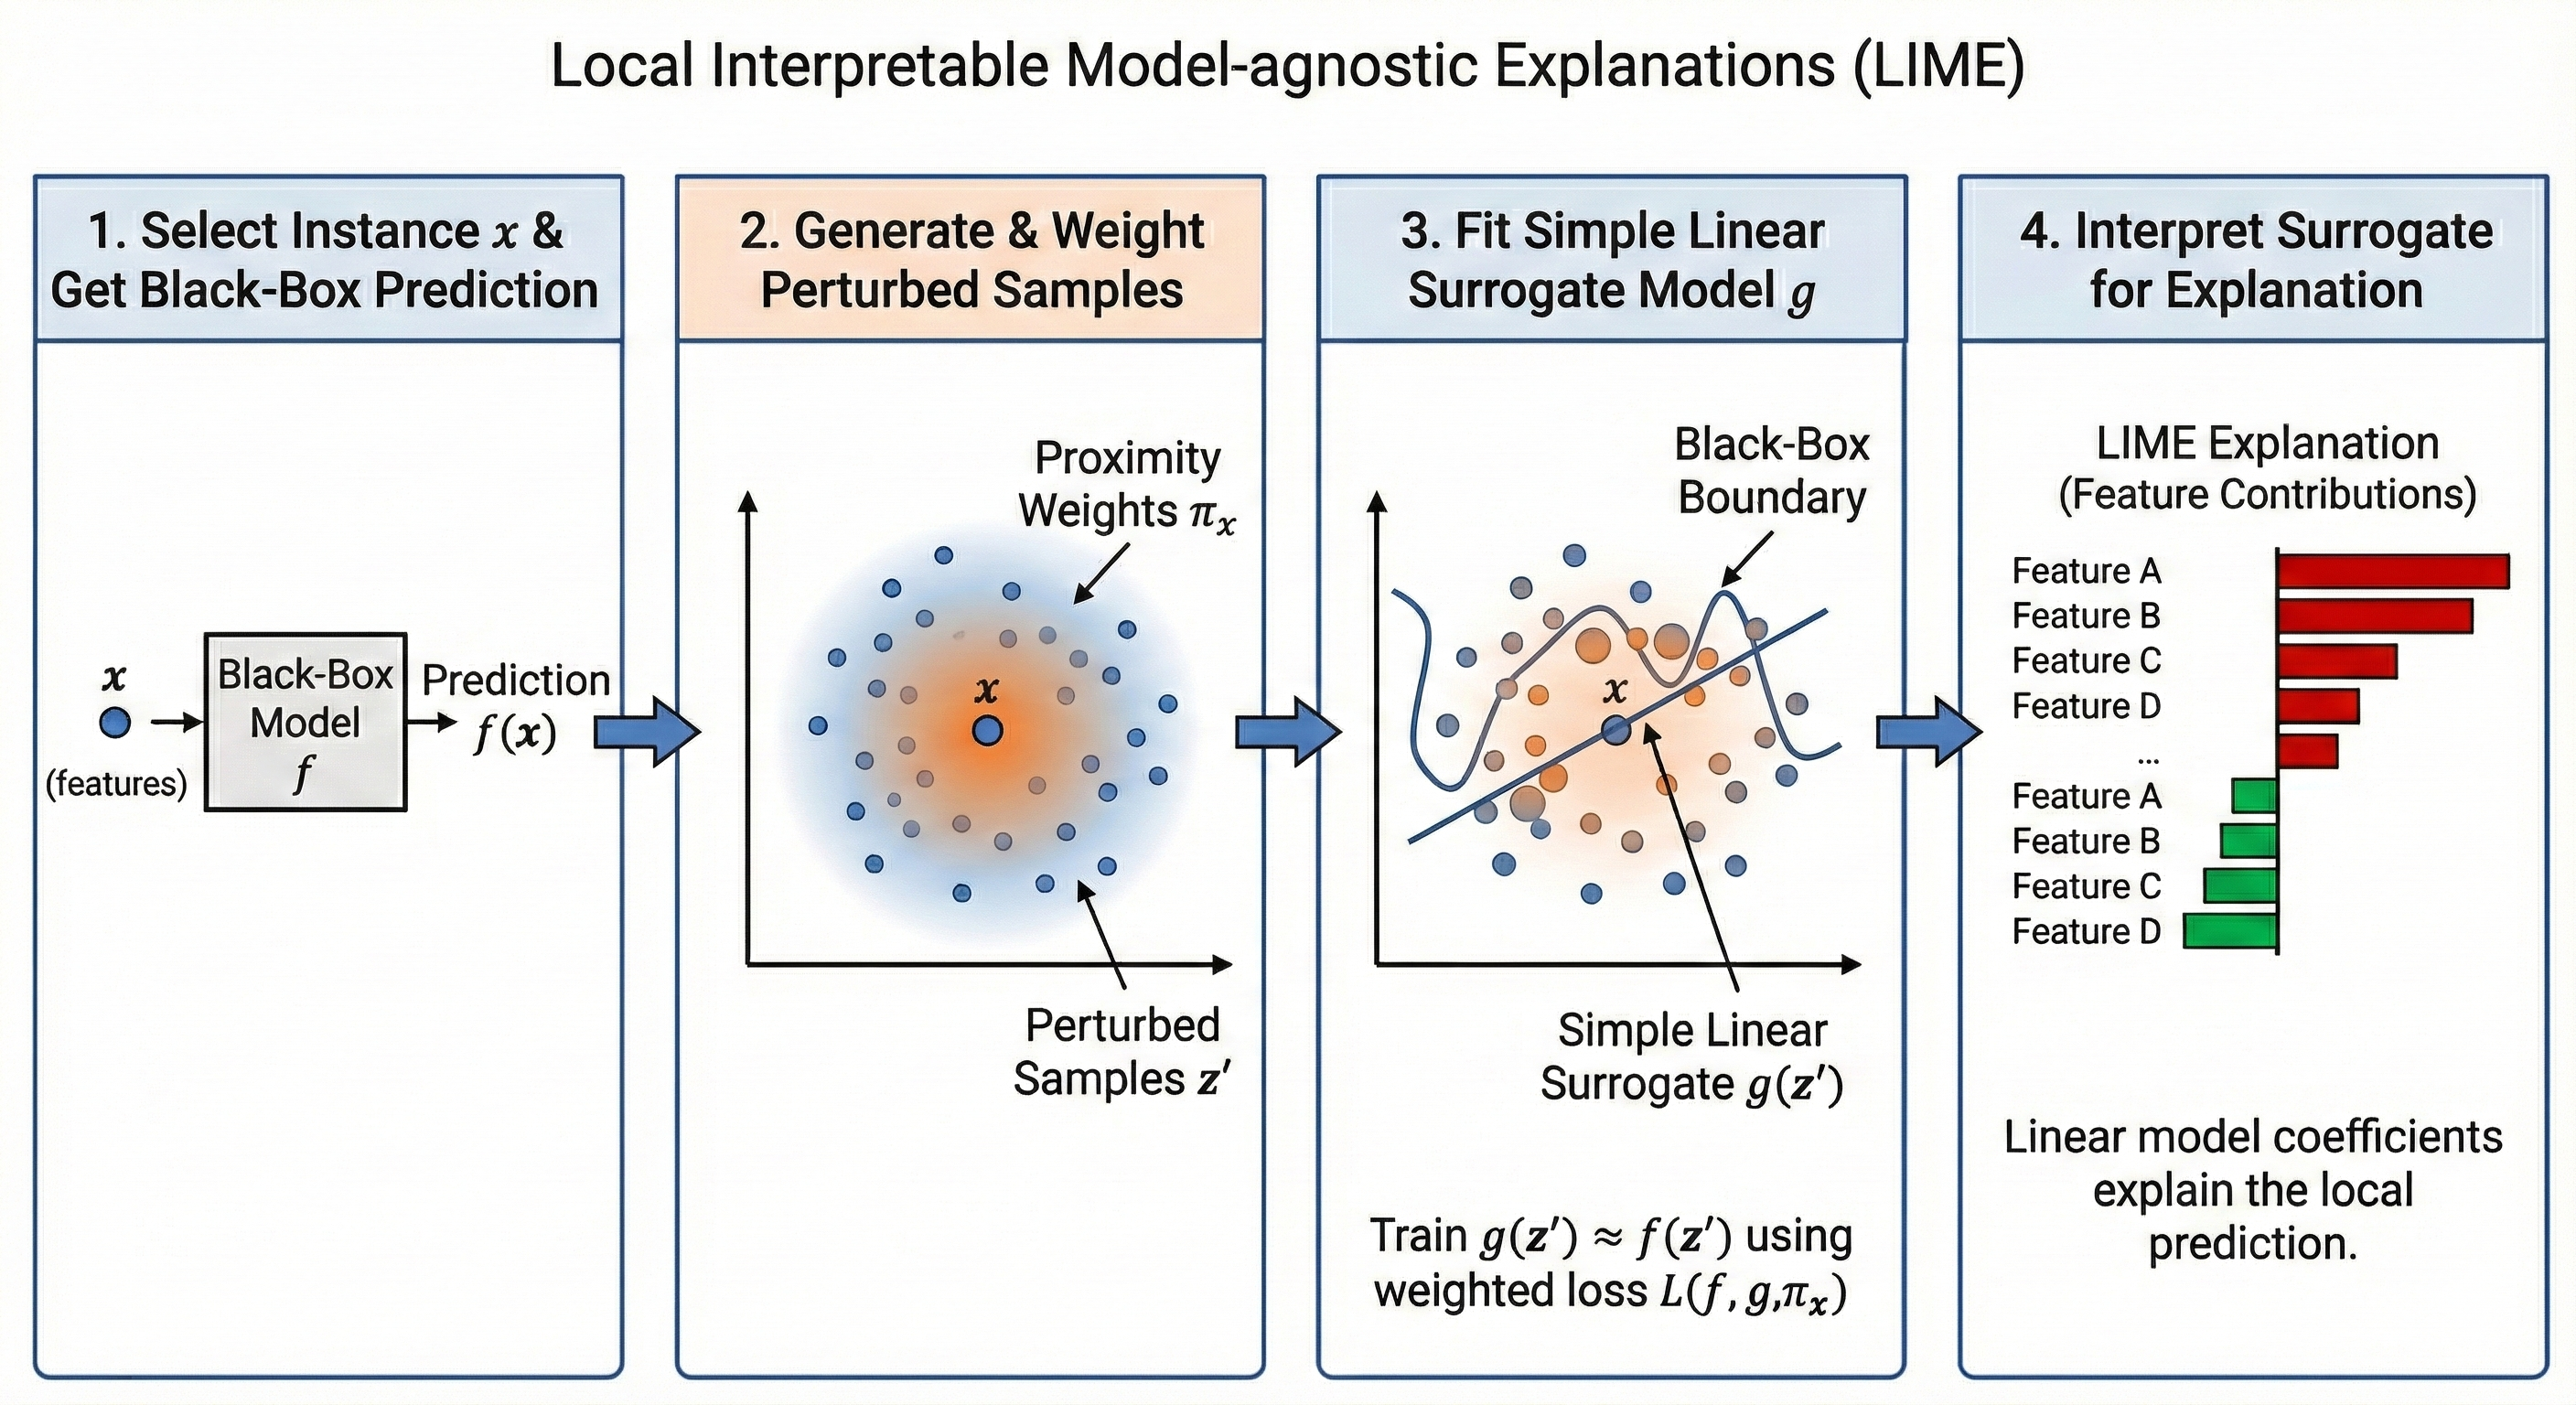
\includegraphics[width=1\textwidth]{imgs/LIME.png}
  \caption[The LIME Architecture]{\textbf{LIME Architecture for Credit Risk}}
  \label{fig:LIME}
\end{figure}

In a consumer credit model including utilisation, recent defaults and income, LIME typically bins features into understandable predicates (e.g.\ utilisation greater than 70\%, at least one default, income greater than 25{,}000 EUR), samples perturbations around the input and trains a sparse linear model. The resulting local surrogate provides a decomposition of PD into a base rate plus additive contributions that mirror a traditional scorecard.

In credit risk, LIME has been applied as a baseline explanation technique to analyse classifiers such as logistic regression, random forests and gradient boosting models \cite{XAiCreditScoring,XAiLiteratureReview2024}. It is used to generate human-readable explanations for individual decisions, compare explanations across model classes and identify potential problems such as over-reliance on specific features or unstable behaviour in local regions.

Several limitations are important in practice:

\begin{itemize}
\item \textit{Stability.}
LIME depends on random sampling of perturbed instances and on the choice of kernel \(\pi_x\). Multiple runs can yield different explanations for the same instance, especially with high-dimensional or highly dependent features \cite{InterpretableModels,SanityChecks}.

\item \textit{Dependence on the perturbation method.}
The perturbation scheme and the mapping between interpretable and original spaces determine which parts of the model are probed. If perturbations stray far from the training data, the surrogate may approximate \(f\) in regions where the model is poorly supported by data.

\item \textit{Correlation among features.}
Credit features are often highly correlated (e.g.\ several indebtedness measures, overlapping delinquency indicators). In such settings, there is no guarantee that LIME’s sparse linear surrogate will distribute importance across correlated variables in a stable or meaningful way, even if the underlying model treats them similarly.
\end{itemize}

These limitations do not preclude the use of LIME, but they motivate combining it with more stable methods such as SHAP in credit applications \cite{XAiCreditScoring,XAiLiteratureReview2024}.

\subsubsection{SHAP: Shapley-Based Additive Explanations}
\label{subsubsec:shap-credit}

\begin{figure}[htbp]
  \centering
  \includegraphics[width=1\textwidth]{imgs/10.jpg}
  \caption[The SHAP Architecture]{\textbf{SHAP Architecture for Credit Risk}}
  \label{fig:SHAP}
\end{figure}

SHAP (SHapley Additive exPlanations) is a family of feature attribution techniques based on cooperative game theory \cite{SHAP}. SHAP views the prediction \( f(x) \) as the “reward” of a coalition of players, where each player is a feature. It computes a unique reward allocation (the Shapley values) that satisfies desirable axioms. For some model classes, including tree ensembles, SHAP can compute exact attributions \cite{SHAP}.

SHAP uses additive explanations of the form
\[
f(x) = \phi_0 + \sum_{j=1}^{M} \phi_j(x),
\]
as in Equation~\eqref{eq:fa-additive}, but defines \(\phi_j(x)\) via Shapley values. Let \(F = \{1,\dots,M\}\) be the set of all features and consider any subset \(S \subseteq F\) that does not contain \(j\). The Shapley value of feature \(j\) at point \(x\) is
\begin{equation}
  \phi_j(x)
  =
  \sum_{S \subseteq F \setminus \{j\}}
  \frac{|S|!\,(M - |S| - 1)!}{M!}\;
  \bigl[
    f_{S \cup \{j\}}(x_{S \cup \{j\}}) - f_S(x_S)
  \bigr],
  \label{eq:shap-definition}
\end{equation}
where \(f_S(x_S)\) is the model prediction when only the features in \(S\) are known and the others are treated as missing (implemented in practice via marginalisation or conditioning over a background distribution). Intuitively, \(\phi_j(x)\) is the average marginal contribution of feature \(j\) across all feature coalitions.

The Shapley value is the only attribution scheme that satisfies local accuracy, missingness, symmetry and a consistency property that prevents attributions from decreasing when a feature’s contribution is increased \cite{SHAP}. These properties are important for comparing models and monitoring their evolution over time.

Computing \eqref{eq:shap-definition} exactly for general models requires evaluating all \(2^M\) feature subsets, which is infeasible for realistic credit datasets. SHAP therefore provides several practical estimators:

\paragraph{KernelSHAP.} KernelSHAP is a model-agnostic approximation that estimates Shapley values by solving a weighted linear regression problem, conceptually similar to LIME but with a kernel that yields Shapley-consistent estimates for linear models \cite{SHAP}. It samples coalitions \(S\), evaluates \(f_S(x_S)\) by marginalising missing features over a background dataset and fits a linear model in coalition space whose coefficients correspond to \(\phi_j(x)\). KernelSHAP applies to any model, including neural networks, but can be computationally heavy for large \(M\) and is sensitive to how missing features are handled, particularly with correlated predictors.

\paragraph{TreeSHAP.} For tree-based models (decision trees, random forests, gradient boosting models such as XGBoost and LightGBM), SHAP offers TreeSHAP \cite{SHAP}. TreeSHAP exploits the tree structure to compute Shapley values in polynomial time by tracking how including or excluding features changes path probabilities and leaf predictions. In credit risk, where tree ensembles are the dominant model in high-performing default prediction systems \cite{XAiCreditRisk2020,XAiCreditAssessment2022,XAiCreditScoring}, TreeSHAP allows institutions to compute instance-level attributions at scale, aggregate them into global importance measures and dependency plots, and generate consistent additive reason codes for accept/reject decisions.

\paragraph{Example in credit scoring.} Consider a PD model based on LTV, arrears and income, implemented as a gradient boosting ensemble. Suppose the background dataset yields an average PD of \(2\%\), which is taken as \(\phi_0\). For a specific borrower \(x\), TreeSHAP might output
\[
\phi_{\text{LTV}}(x) = +3.2\%,\quad
\phi_{\text{arrears}}(x) = +2.9\%,\quad
\phi_{\text{income}}(x) = -0.8\%,\quad
\text{others combined} = +0.7\%,
\]
so that
\[
f(x) = 2.0\% + 3.2\% + 2.9\% - 0.8\% + 0.7\% = 8.0\%.
\]
This mirrors the LIME-style decomposition but satisfies the Shapley axioms. If the bank updates the model so that high LTV has more impact on PD, LTV’s Shapley attribution cannot decrease.

\paragraph{Other SHAP variants.} The SHAP library includes model-specific variants such as LinearSHAP for linear models and DeepSHAP for certain neural architectures. SHAP interaction values can measure pairwise interaction effects \cite{SHAP}. In credit scoring, TreeSHAP is the default choice for tree ensembles \cite{XAiLiteratureReview2024,XAiFinanceReview2025}.

\subsubsection{Portfolio-Level Analyses Using Feature Attributions}
\label{subsubsec:fa-portfolio}

Beyond explaining individual decisions, feature attributions support portfolio-level diagnostics and model management, especially due to the additive structure of SHAP.

Typical use cases include:
\begin{itemize}
\item \emph{Global importance rankings}: risk managers compute SHAP values \(\phi_j(x^{(n)})\) for each loan and average \(|\phi_j|\) across the portfolio to obtain a ranking of drivers. These rankings are compared with prior expectations and policies, and unexpected drivers can flag potential proxies or artefacts \cite{XAiCreditRisk2020,XAiCreditAssessment2022}.

\item \emph{Partial dependence and SHAP dependence}: partial and SHAP dependence plots show how predicted PD varies with a single feature, holding other inputs fixed or marginalised. They are used to check monotone patterns (e.g.\ PD increasing with LTV up to a threshold) and heterogeneous effects across ranges (e.g.\ income having stronger marginal impact for low-income borrowers) \cite{XAiCreditScoring,XAiLiteratureReview2024}.

\item \emph{Segment-specific analyses}: feature attributions can be computed within segments (retail vs.\ SME, mortgage vs.\ unsecured, geographic regions) to see how drivers change across products and customer groups. Behavioural features tend to dominate for mature credit-card customers, whereas application variables are more important at origination and for instalment loans \cite{XAiCreditScoring,XAiCreditAssessment2022}.

\item \emph{Stress-testing and scenario analysis}: in stress tests, feature attributions help explain why portfolio PDs rise under adverse macro scenarios. Central banks and banks can quantify how variables such as unemployment or house prices contribute to PD changes and which segments are most exposed \cite{XAiDefaultRisk2019,XAiFinancialRisk}.
\end{itemize}

\subsubsection{Empirical Evidence and Comparative Assessment in Credit Risk}
\label{subsubsec:fa-evidence-comparison}

Empirical studies generally find that feature-attribution tools align well with established credit-risk knowledge. Bussmann et al.\ \cite{XAiCreditRisk2020} show that TreeSHAP importance rankings for a corporate XGBoost model largely match expert assessments, with leverage, profitability and cash-flow emerging as dominant drivers. In consumer credit, TreeSHAP applied to LightGBM highlights utilisation, arrears status and payment behaviour as key features, consistent with traditional scorecards \cite{XAiCreditAssessment2022}. LIME can surface similar patterns, but its sensitivity to sampling choices makes systematic validation more difficult \cite{XAiCreditScoring}.

Across studies, SHAP is typically found to provide more stable attributions than LIME when inputs or background samples are perturbed, reflecting the deterministic nature of TreeSHAP for tree ensembles. SHAP’s additive decompositions, which sum to the model prediction, facilitate the generation of natural-language reason codes and large-scale monitoring over portfolios \cite{XAiCreditAssessment2022,XAiFinanceReview2025}. By contrast, LIME’s local surrogate models are more computationally demanding to apply portfolio-wide and its variability complicates robustness checks and fairness diagnostics \cite{XAiCreditScoring,XAiLiteratureReview2024}.

\subsubsection{Strengths and Limitations of Feature Attribution in Credit Risk}
\label{subsubsec:fa-strengths-limitations}

\paragraph{Strengths.}
\begin{itemize}
\item \emph{Individual and portfolio-level insight.} Local attributions support case-level justification and remediation suggestions, while aggregations across loans provide global views of risk drivers and enable model debugging.

\item \emph{Model-agnostic explanations with additivity.} KernelSHAP and LIME can be applied to any black-box model (tree ensembles, neural networks, hybrid architectures), and TreeSHAP offers fast, exact attributions for tree-based models commonly used in credit scoring. The additive property of SHAP values underpins consistent decompositions into reason codes.

\item \emph{Support for fairness diagnostics.} Comparing attributions across groups or segments allows practitioners to detect potential reliance on protected attributes or proxies and to assess whether dominant drivers are economically plausible \cite{XAiFinancialRisk,InterpretableModels}.
\end{itemize}

\paragraph{Limitations.}
\begin{itemize}
\item \emph{Correlation and background dependence.} Feature attributions describe how the model uses inputs, not causal effects. The way importance is shared among correlated variables depends on the background dataset and modelling choices, limiting the use of attributions for policy conclusions or strong fairness claims.

\item \emph{Stability and robustness.} Although TreeSHAP is deterministic for a fixed model and background set, explanations can change after retraining, portfolio shifts or background updates. LIME adds further variability through random sampling. Ensuring explanations are stable enough for regulatory reporting remains an open challenge \cite{SanityChecks,XAiFinanceReview2025}.

\item \emph{Cognitive load and actionability.} High-dimensional explanations can overwhelm users, so operational deployments usually restrict attention to a small set of top features per borrower. This simplifies communication but can hide interactions and makes it difficult to connect explanations to feasible recourse plans when business, legal or causal constraints apply \cite{InterpretableModels,XAiCreditScoring,Counterfactual,XAiFinancialRisk}.
\end{itemize}

Feature attribution methods (particularly SHAP and, to a lesser extent, LIME) are therefore the current workhorses for explaining complex credit scoring models. They allow institutions to exploit the predictive gains of tree ensembles while retaining a degree of transparency suitable for risk management and supervisory dialogue, but must be embedded within broader model risk management practices.

\subsection{Counterfactual Explanations for Accept/Reject Decisions}
\label{subsec:counterfactuals}

Counterfactual explanations approach explanations from a different angle than feature attribution. Instead of asking \emph{why} the model assigned a given PD to the borrower, they ask \emph{what would need to change} in the borrower’s characteristics for the model to yield a more favourable decision (typically, loan acceptance or a lower risk classification) \cite{Counterfactual}. For example:

\begin{quote}
“Your loan was rejected because your debt-to-income ratio is 0.55 and you have two recent delinquencies. If your debt-to-income ratio were less than 0.40 and you had no delinquencies during the last 12 months, the loan would have been accepted.”
\end{quote}

This formulation explains both why the loan was denied and which actions might lead to a different decision.

Counterfactuals are particularly relevant in regulated consumer credit markets in which laws such as GDPR and ECOA require lenders to provide rationales for denying loans and, in some readings, to enable consumers to contest or modify those decisions~\cite{Counterfactual,XAiFinancialRisk}. The following subsections outline their optimisation-based formulation, credit-specific constraints and empirical evidence.

\subsubsection{Problem Formulation and Recourse}
\label{subsubsec:cf-formulation}

Let \(x = (x_1,\dots,x_M)\) denote the feature vector of a borrower (for example, income, age, outstanding debt, delinquencies, LTV) and let \(f(x)\) be a trained model that outputs a PD or a continuous risk score. For simplicity, consider a binary classifier
\[
\hat{y}(x)
= \mathbf{1}\{f(x) \ge \tau\},
\]
where \(\tau\) is a decision threshold (e.g.\ a PD cut-off). Suppose the current application is rejected, \(\hat{y}(x) = 0\), and the applicant wishes to know how to obtain an approval. A \emph{counterfactual explanation} seeks an alternative feature vector \(x'\) that satisfies two requirements~\cite{Counterfactual}:

\begin{enumerate}
  \item \textbf{Outcome requirement:} the model assigns a desired outcome to \(x'\), for example
  \[
  \hat{y}(x') = 1
  \quad\text{or}\quad
  f(x') \ge \tau^*,
  \]
  where \(\tau^*\) may be stricter than the original boundary to provide a safety margin.
  \item \textbf{Proximity requirement:} the counterfactual \(x'\) should be ``close'' to the original \(x\) under a suitable distance or cost function \(d(x,x')\), so that the suggested changes are minimal and realistic.
\end{enumerate}

These requirements are typically combined into an optimisation problem
\begin{equation}
  \label{eq:cf-optimisation}
  \min_{x'}\;
  d(x,x') + \lambda\,\ell\bigl(f(x'), y^{\star}\bigr)
  \quad\text{subject to}\quad
  x' \in \mathcal{F},
\end{equation}
where:
\begin{itemize}
  \item \(d(x,x')\) measures the cost of moving from \(x\) to \(x'\) (for example, a weighted \(\ell_1\) or \(\ell_2\) distance);
  \item \(\ell(f(x'), y^{\star})\) penalises deviations of the model output from a target outcome \(y^{\star}\);
  \item \(\lambda > 0\) controls the trade-off between outcome satisfaction and proximity;
  \item \(\mathcal{F}\) encodes feasibility constraints (e.g.\ bounds, monotonic relationships, business rules).
\end{itemize}

\begin{figure}[htbp]
  \centering
  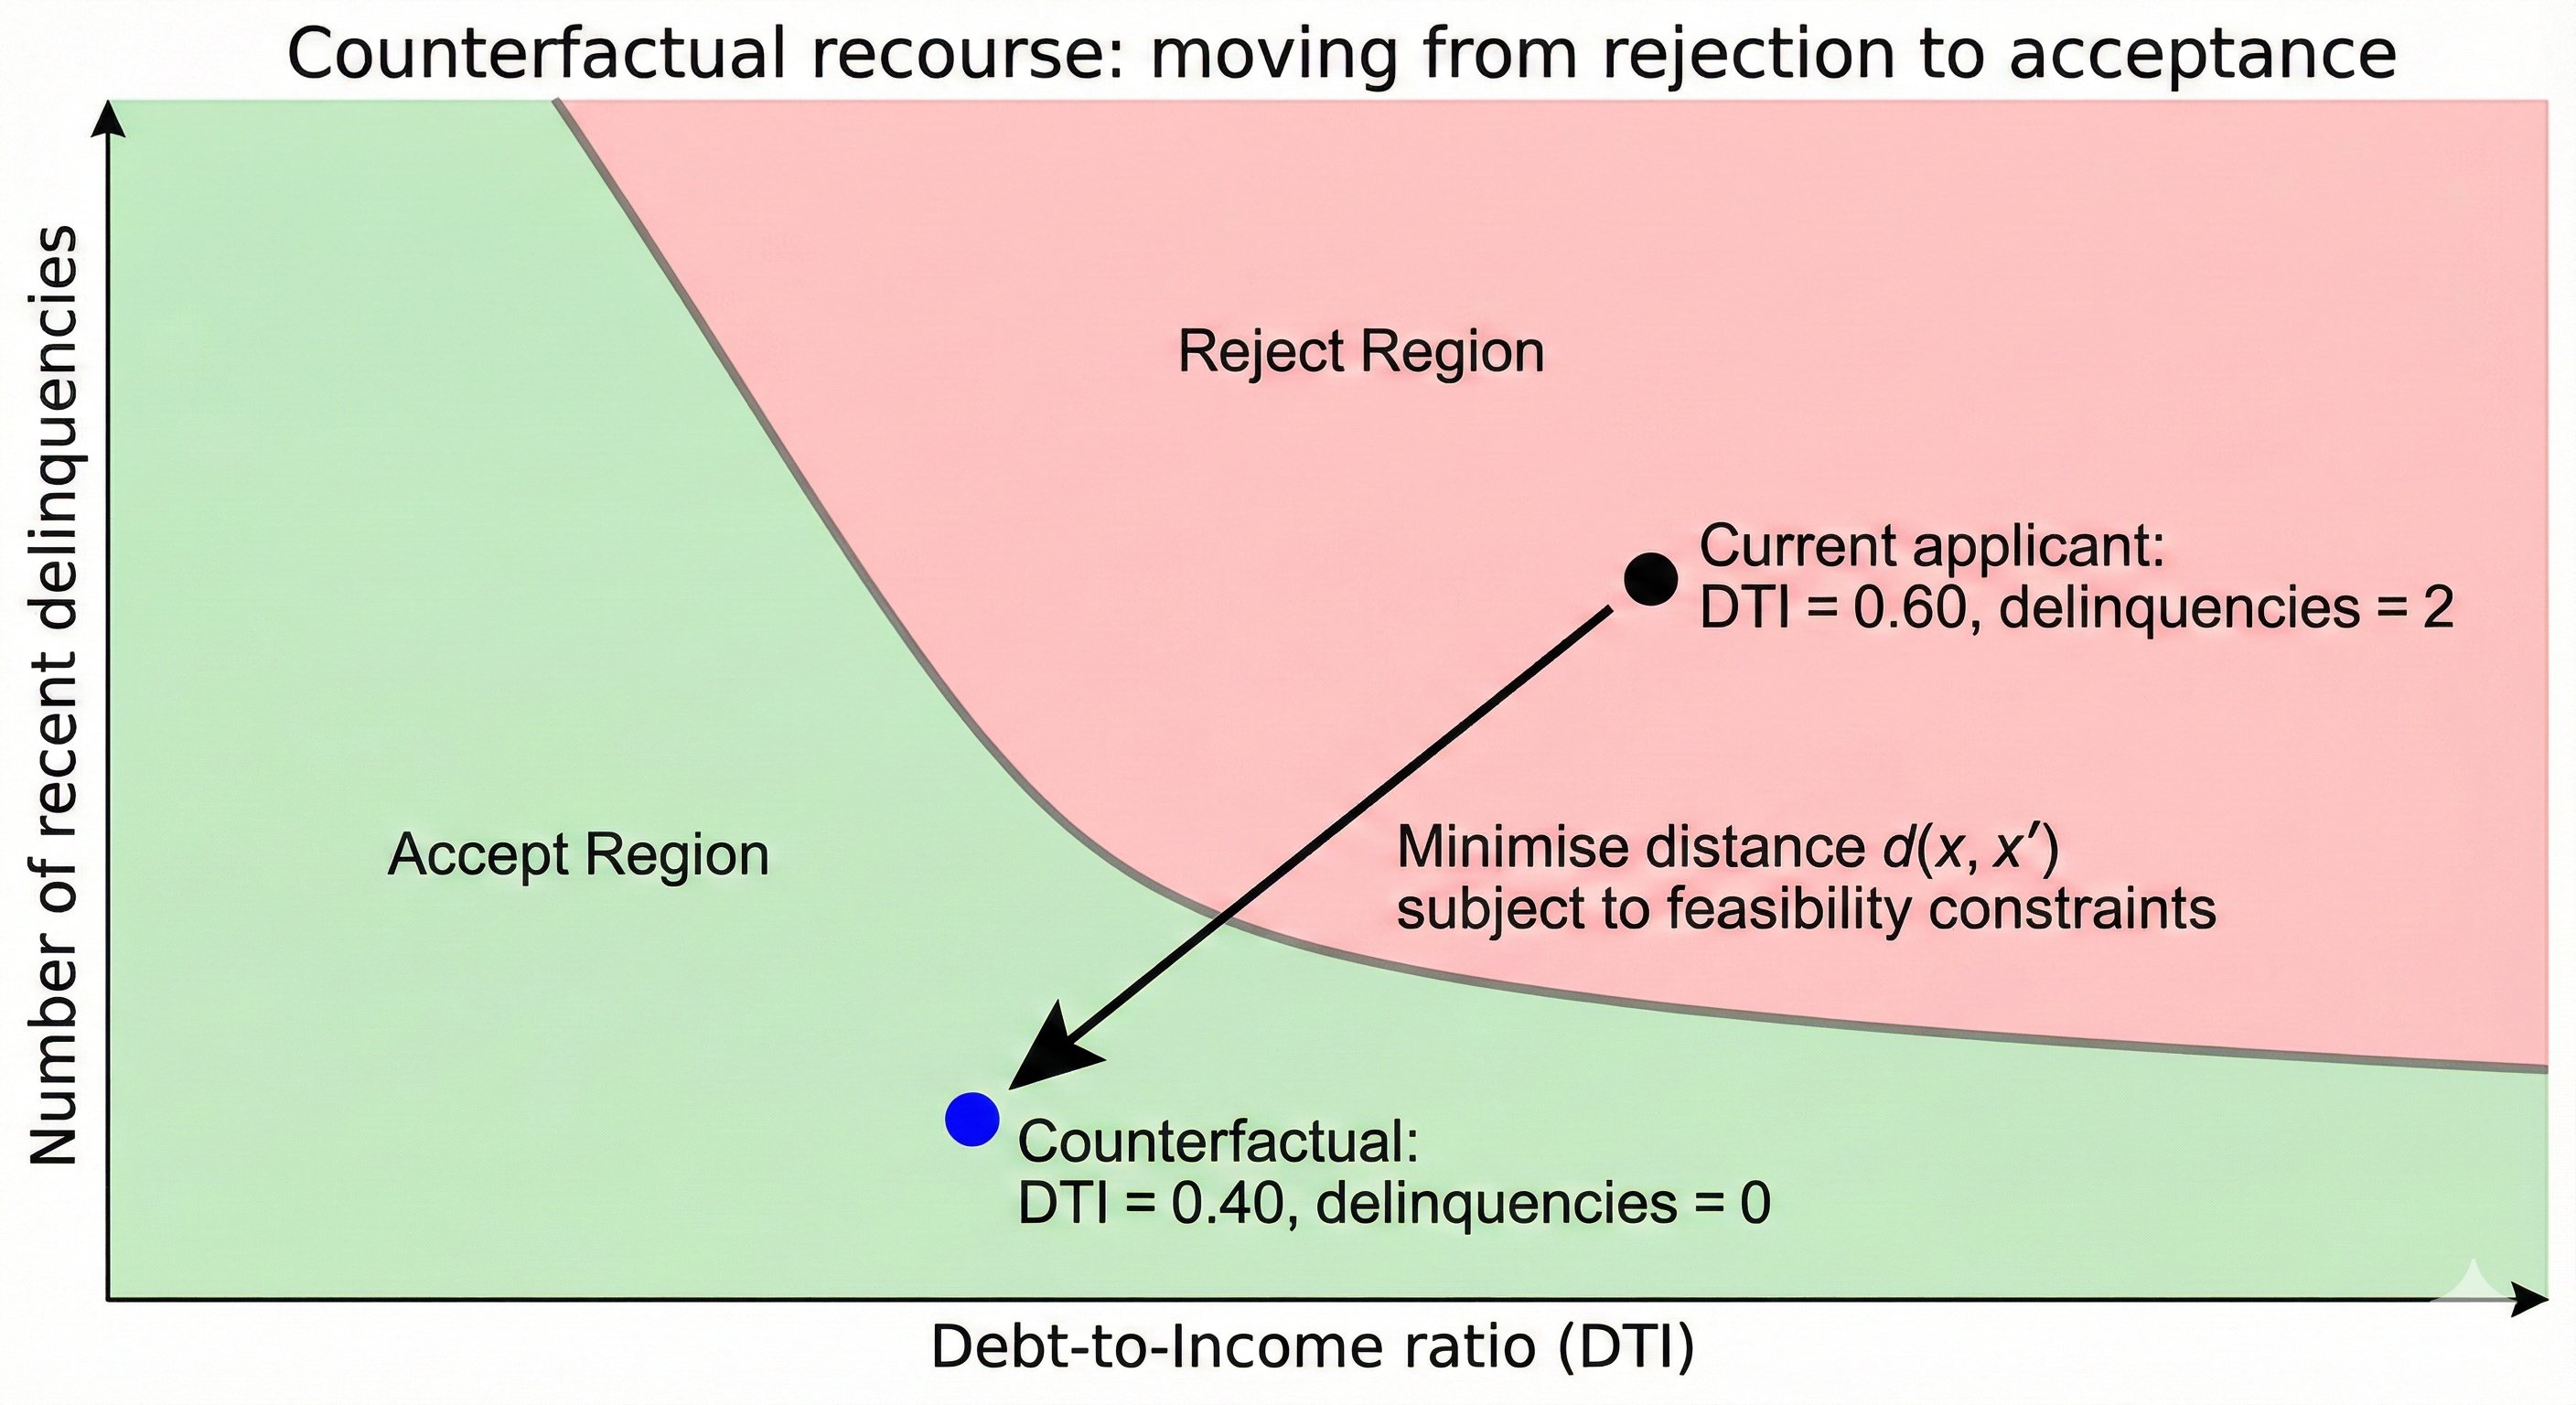
\includegraphics[width=0.8\textwidth]{imgs/Counterfactuals.png}
  \caption[Counterfactual recourse illustration.]{\textbf{Counterfactual recourse illustration.} The plot shows how a rejected applicant at point \(x\) in the high-DTI, high-delinquency region can move minimally to a nearby point \(x'\) across the decision boundary into the acceptance region.}
  \label{fig:counterfactuals}
\end{figure}

In the formulation of Wachter et al.~\cite{Counterfactual}, the distance \(d(x,x')\) is a normalised \(\ell_1\) or \(\ell_2\) distance and the loss term encourages \(f(x')\) to reach a user-specified target value, with \(\lambda\) tuned until the target is met. Credit-focused work refines this by adopting domain-specific distances, constraining immutable features and generating multiple counterfactuals~\cite{XAiCreditDecision,XAiCreditScoring}.

A simple example: suppose a gradient boosting model \(f(x)\) outputs a one-year PD and accepts applications with \(f(x) < 0.05\). Consider a borrower with
\[
\text{income} = 30{,}000\ \text{EUR},\quad
\text{DTI} = 0.60,\quad
\text{recent delinquencies} = 2,
\]
for which the model predicts \(f(x) = 0.12\). A counterfactual might be
\[
 x'
 : \quad
 \text{income} = 30{,}000\ \text{EUR},\quad
 \text{DTI} = 0.40,\quad
 \text{delinquencies} = 0,
\]
with \(f(x') = 0.03 < 0.05\). From the borrower’s perspective, this both justifies the rejection and indicates a direction for improvement.

\subsubsection{Actionability, Feasibility and Constraints}
\label{subsubsec:cf-actionability}

The optimisation problem~\eqref{eq:cf-optimisation} is meaningful only if the feasible set \(\mathcal{F}\) and distance \(d(x,x')\) reflect what can realistically change. In credit scoring:

\begin{itemize}
  \item \emph{Immutable} features (age, historical defaults) must be held fixed.
  \item \emph{Hard-to-change} features (education, occupation, region) may change only over long horizons and at high cost.
  \item \emph{Actionable} features (utilisation of existing credit lines, requested loan size, voluntary prepayments) are accessible levers.
\end{itemize}

Credit-focused counterfactual methods therefore partition features into immutable, slowly mutable and actionable subsets, constrain changes to the latter and weight the distance function accordingly~\cite{XAiCreditDecision,XAiCreditScoring}. A common choice is a weighted \(\ell_1\) distance
\[
d(x,x')
= \sum_{j=1}^{M} w_j\,|x_j - x'_j|,
\]
with large weights on hard-to-change features to discourage unrealistic suggestions.

Categorical and discrete features (employment type, home ownership, delinquency flags) require special treatment. Gradient-based optimisation is not directly applicable, so mixed-integer, combinatorial or heuristic search methods (e.g.\ greedy or beam search, constraint programming, sampling-based approximations) are used to explore plausible local perturbations while remaining on the data manifold~\cite{XAiCreditDecision,XAiCreditScoring}.

A distinction arises between \textit{individual recourse} and \textit{group-level fairness}. Individual recourse focuses on feasible changes for a single borrower; group-level analyses examine whether recourse is systematically easier for some groups than others. Recent work combines counterfactual explanations with group fairness metrics to detect and mitigate such disparities~\cite{Counterfactual,XAiFinancialRisk}, directly connecting to the issues in Section~\ref{subsec:fairness-bias}.

\subsubsection{Applications in Credit Scoring and Lending}
\label{subsubsec:cf-credit-applications}

Counterfactual explanations have been implemented in many credit scoring and lending studies, typically by combining a high-performing classifier (often a gradient boosting decision tree trained on datasets such as FICO HELOC, German Credit or Taiwan Credit Card) with an optimisation-based recourse procedure. The main objectives are to provide borrowers with concrete examples of how to improve their credit profiles, to give loan officers visibility into model behaviour near decision boundaries and to study how different explanation formats affect perceived fairness and understanding~\cite{XAiConsumers,XAiCreditDecision,XAiCreditScoring}.

A common setup trains an XGBoost model to predict default and, for each rejected applicant, searches for minimally changed profiles whose predicted PD falls below the rejection threshold. Many rejected applicants admit counterfactuals requiring moderate adjustments (e.g.\ small reductions in utilisation or modest changes in requested loan amount), and aggregating these suggestions yields a global view of which behavioural changes most frequently move applicants from rejection to acceptance~\cite{XAiCreditDecision,XAiCreditScoring}. 

Experimental user studies compare such counterfactual recommendations with feature-importance lists or rule summaries. Non-expert participants generally rate counterfactuals as more actionable and easier to understand, because they explicitly specify how outcomes could change, although overly complex or unrealistic counterfactuals reduce trust~\cite{XAiConsumers}. Regulators and central banks have explored related ideas in stress-testing and mortgage risk work, using counterfactual analyses to characterise borrower profiles that default under adverse but not baseline scenarios and to understand how changes in income, interest rates and house prices push borrowers across default thresholds~\cite{XAiDefaultRisk2019,XAiFinancialRisk}.

\subsubsection{Strengths and Limitations in Credit Risk}
\label{subsubsec:cf-strengths-limitations}

\paragraph{Strengths.}
\begin{itemize}
  \item \emph{Actionability and recourse.} Counterfactuals answer “what could be changed to obtain a different decision?”, aligning with recourse-oriented regulation and borrower expectations~\cite{Counterfactual,XAiCreditDecision}.
  \item \emph{Local decision-boundary insight.} Because counterfactuals are constructed near the accept–reject boundary, they reveal which features drive transitions between approval and rejection regions.
  \item \emph{Model-agnostic applicability.} Counterfactual generators treat the predictor as a black box and can be applied to the same gradient boosting and neural network models used for high-performance credit scoring~\cite{XAiCreditScoring,XAiLiteratureReview2024}.
\end{itemize}

\paragraph{Limitations.}
\begin{itemize}
  \item \emph{Non-uniqueness and selection.} Many distinct counterfactuals can flip a decision. Choosing which one to present (closest, cheapest, diverse set) introduces design choices and may create disparities in recourse across groups~\cite{Counterfactual,XAiConsumers,XAiFinancialRisk}.
  \item \emph{Feasibility and causal consistency.} Optimising over observational features does not guarantee realistic or economically plausible trajectories (e.g.\ removing past delinquencies, jointly increasing income while reducing working hours). Enforcing structural or causal constraints is technically demanding and remains an active research area~\cite{Counterfactual,XAiFinancialRisk}.
  \item \emph{Sensitivity and scalability.} Counterfactuals can expose sensitive dependencies (e.g.\ incentives to move postcode or change occupation) and thus highlight proxies for protected attributes~\cite{XAiFinancialRisk,InterpretableModels}. Generating counterfactuals requires solving an optimisation problem per instance; large portfolios or real-time systems often rely on approximations that may sacrifice optimality~\cite{XAiCreditDecision,XAiCreditScoring}.
  \item \emph{Consistency with other explanations.} Counterfactuals and feature attributions can emphasise different aspects of the same decision (for instance, SHAP highlighting income while the closest counterfactual mainly changes utilisation). Reconciling these differences, given feasibility and cost constraints on recourse, remains an open issue~\cite{XAiFinanceReview2025,XAiLiteratureReview2024}.
\end{itemize}

In short, counterfactual explanations translate model output into potential actions, while feature attribution decomposes the current prediction. Model risk managers and regulators also require portfolio-level summaries of model logic, which motivates surrogate and rule-based explanations.

\subsubsection{Global Surrogate Models and Model Distillation}
\label{subsubsec:surrogates-formulation}

Let \(f : \mathcal{X} \to \mathcal{Y}\) be a trained black-box model for credit risk, such as a gradient boosting ensemble that outputs PDs. A \emph{global surrogate model} is an interpretable model \(g : \mathcal{X} \to \mathcal{Y}\) (e.g.\ a shallow decision tree or sparse logistic regression) trained to approximate \(f\) on a suitable set of inputs. Given a dataset \(\{x^{(n)}\}_{n=1}^{N}\), the surrogate is obtained by solving
\begin{equation}
  \label{eq:surrogate-optimisation}
  \hat{g}
  = \arg\min_{g \in \mathcal{G}}
    \frac{1}{N} \sum_{n=1}^{N}
      L\bigl(g(x^{(n)}), f(x^{(n)})\bigr)
    + \Omega(g),
\end{equation}
where:
\begin{itemize}
  \item \(\mathcal{G}\) is a class of interpretable models, such as depth-limited trees, sparse linear models or monotone generalised additive models \cite{InterpretableModels};
  \item \(L\) measures disagreement between surrogate and black-box model (e.g.\ squared error on PDs or cross-entropy between class probabilities);
  \item \(\Omega(g)\) is a complexity penalty that encourages simplicity (e.g.\ limits on tree depth or number of non-zero coefficients).
\end{itemize}
This “model distillation” setup mirrors knowledge distillation in deep learning, but the student model is explicitly constrained to be interpretable \cite{InterpretableModels,XAiFinanceReview2025}.

For example, suppose \(f\) is a LightGBM model for one-year PDs on consumer loans. Choosing \(\mathcal{G}\) as trees of depth at most three and training \(g\) to minimise squared error with respect to \(f(x^{(n)})\) might yield rules such as:
\begin{quote}
\begin{itemize}
  \item If \(\text{delinquencies} \ge 2\) and \(\text{utilisation} > 80\%\), then \(\widehat{\mathrm{PD}} \approx 18\%\).
  \item Else if \(\text{delinquencies} = 0\) and \(\text{loan-to-income} < 3\), then \(\widehat{\mathrm{PD}} \approx 1.5\%\).
  \item Otherwise, \(\widehat{\mathrm{PD}} \approx 6\%\).
\end{itemize}
\end{quote}
Even if the underlying model uses many more features and interactions, the surrogate provides a compact portfolio-level summary of its main logic.

Surrogate fidelity must be evaluated explicitly, for instance via:
\begin{itemize}
  \item \(R^2\) or mean squared error between \(g(x^{(n)})\) and \(f(x^{(n)})\) on validation data;
  \item the fraction of instances for which \(g\) and \(f\) agree on accept/reject decisions;
  \item comparisons of score distributions or calibration plots across segments.
\end{itemize}
If fidelity is low, the surrogate should not be presented as an explanation of \(f\) \cite{InterpretableModels,XAiFinancialRisk}.

Surrogates can also be constrained to reflect domain knowledge, for example monotonicity in delinquency counts or utilisation, or restrictions on which features may appear. This links to interpretable risk modelling practices and allows the surrogate to function both as an approximation of \(f\) and as a normative template for how risk should depend on key variables \cite{InterpretableModels,XAiFinanceReview2025}.

\subsubsection{Rule Lists, Decision Sets and Anchors}
\label{subsubsec:rules-anchors}

Many users prefer explanations in the form of explicit if–then rules. Rule lists and decision sets approximate a black-box predictor by collections of human-readable rules that partition the input space into interpretable segments, each associated with a predicted risk level or decision \cite{InterpretableModels,Anchors}. They can serve as standalone interpretable models or as surrogates for complex models.

A \emph{rule list} is an ordered sequence of rules:
\[
\text{if condition}_1 \text{ then outcome}_1; \quad
\text{else if condition}_2 \text{ then outcome}_2; \quad
\ldots; \quad
\text{else outcome}_{\text{default}},
\]
where each condition is a conjunction of simple predicates (e.g.\ thresholds on numerical variables or specific categories). For credit scoring, a rule list might be:
\begin{quote}
\begin{itemize}
  \item If \(\text{delinquencies} \ge 2\) and \(\text{DTI} > 0.5\), then \(\widehat{\mathrm{PD}} = 0.20\).
  \item Else if \(\text{delinquencies} = 1\) and \(\text{DTI} > 0.6\), then \(\widehat{\mathrm{PD}} = 0.15\).
  \item Else if \(\text{delinquencies} = 0\) and \(\text{loan-to-income} < 3\), then \(\widehat{\mathrm{PD}} = 0.02\).
  \item Else \(\widehat{\mathrm{PD}} = 0.07\).
\end{itemize}
\end{quote}
Such a list can be obtained by training a rule-learning algorithm to mimic \(f\) under a complexity penalty limiting the number and length of rules \cite{InterpretableModels}.

\emph{Decision sets} drop the ordering requirement: they consist of an unordered collection of rules, each covering a region of the input space, with conflicts resolved by aggregation schemes. This format is useful when multiple rules may apply to the same borrower, for example to highlight several reasons for heightened risk.

Anchors \cite{Anchors} sit between local and global rule-based explanations. An \emph{anchor} is a high-precision if–then rule that “anchors” the model prediction in a local region: whenever the conditions in the rule are satisfied, the model output is very likely to match the original prediction. Given an instance \(x\) and classifier \(f\), an anchor rule
\[
\text{if } A(x) \text{ then predict } \hat{y}
\]
is constructed such that:
\begin{itemize}
  \item among synthetic samples \(z\) satisfying \(A(z)\), the fraction with \(f(z) = \hat{y}\) exceeds a precision threshold (e.g.\ 95\%);
  \item coverage is sufficiently high in the local data distribution.
\end{itemize}
For a rejected credit application, an anchor might be:
\begin{quote}
\emph{If} (delinquencies \(\ge 2\)) \emph{and} (utilisation \(> 90\%\)), \emph{then} the model predicts rejection with probability at least 0.98.
\end{quote}
This rule provides a crisp characterisation of a region where the model behaves consistently and can be translated into reason codes or policy statements.

Compared with SHAP and LIME, rule-based explanations:
\begin{itemize}
  \item align closely with existing practices such as scorecards and policy rules, easing adoption by loan officers and regulators \cite{InterpretableModels,XAiCreditScoring};
  \item can express non-linear interactions explicitly (e.g.\ joint conditions on DTI and delinquencies);
  \item naturally support segmentation analysis via explicit risk buckets or decision regions.
\end{itemize}
Their main challenges are combinatorial (search in high-dimensional spaces) and the fidelity–simplicity trade-off, as discussed below.

\subsubsection{Applications and Evidence in Credit Risk}
\label{subsubsec:surrogates-credit-applications}

Empirical work on surrogate and rule-based explanations in credit risk is less extensive than for feature attribution, but several patterns recur \cite{InterpretableModels,XAiCreditRisk2020,XAiCreditAssessment2022,XAiCreditScoring,XAiLiteratureReview2024,XAiFinancialRisk}.

Global surrogates are mainly used as diagnostic and communication tools for gradient boosting models. In a corporate credit risk study where XGBoost substantially outperformed logistic regression, the authors trained a shallow decision tree on the XGBoost outputs and compared its rules with those of a traditional rating model \cite{XAiCreditRisk2020}. The surrogate captured a small number of dominant interaction patterns (e.g.\ leverage, profit margins, interest coverage) consistent with rating experts’ expectations, while higher-order interactions remained opaque in the full model.

For consumer credit, rule lists and decision sets have been studied both as primary models and as surrogates. In HELOC-like datasets, sparse rule lists trained on labels achieved accuracy comparable to logistic regression but clearly below gradient boosting. When trained to mimic a GBDT model, rule lists could match the complex model’s accept/reject decisions with high agreement (around 90–95\%) while providing concise, human-readable policies \cite{InterpretableModels,XAiCreditScoring}. This motivates a hybrid pattern: use the black-box model operationally, but document and discuss its behaviour via rule-based surrogates.

Local rule-based methods such as Anchors have been applied to borderline applicants to generate compact conditions that “lock in” the model’s decision. Experimental studies indicate that practitioners often prefer such rule-style explanations over raw feature importance vectors because they resemble existing underwriting rules and are easier to communicate \cite{Anchors,XAiCreditScoring,XAiConsumers}.

Supervisory authorities and central banks acknowledge the usefulness of surrogate and rule-based explanations but emphasise that they must be treated as approximations. Model risk guidelines stress that any surrogate used in regulatory communication should be accompanied by explicit fidelity metrics and disclosure of where the surrogate diverges from the underlying model \cite{XAiFinancialRisk}, to avoid “explanation by proxy”.

\subsubsection{Strengths, Limitations and Interplay with Other XAI Methods}
\label{subsubsec:surrogates-strengths-limitations}

Surrogate and rule-based methods sit between local feature attribution and individual counterfactual explanations.

On the positive side:
\begin{itemize}
  \item they summarise how key features and interactions influence PD and approve/reject decisions across the portfolio, supporting policy and capital discussions;
  \item rule-based explanations (trees, lists, scorecards) closely resemble traditional credit models and fit existing governance and documentation practices \cite{InterpretableModels,XAiCreditScoring};
  \item comparing surrogate rules with black-box outputs highlights regions where model behaviour appears inconsistent with lending policies (e.g.\ non-monotonic responses to delinquency or LTV), guiding model refinements.
\end{itemize}

Key disadvantages include:
\begin{itemize}
  \item \emph{Fidelity–simplicity trade-off}. Simple surrogates may miss important interactions, especially in heterogeneous portfolios, while highly faithful surrogates can become large and unwieldy. Fidelity must be quantified and reported explicitly \cite{InterpretableModels,XAiFinancialRisk}.
  \item \emph{Risk of misplaced trust}. Users may treat the surrogate as the “real” model. If fidelity is low in some regions, surrogates can mislead stakeholders about which drivers matter for particular subpopulations or scenarios \cite{XAiFinancialRisk,XAiFinanceReview2025}.
  \item \emph{Combinatorial complexity}. High-dimensional credit data with many categorical variables and interactions make it costly to search for small, accurate rule sets; heuristic search performance depends strongly on hyperparameters and sample design \cite{InterpretableModels,Anchors}.
  \item \emph{No guarantee of causal validity}. As with feature attributions and counterfactuals, surrogate rules reflect patterns in model outputs, not causal relationships. Rules such as “high utilisation and postcode in region A implies high PD” may simply capture proxies for socioeconomic status or protected characteristics \cite{InterpretableModels,XAiFinancialRisk}.
\end{itemize}

In practice, surrogate and rule-based explanations are most effective when combined with other XAI tools: SHAP-like methods provide local and global attributions; counterfactuals clarify feasible recourse; and global surrogates and rule lists summarise portfolio-level behaviour for governance and regulatory dialogue.

\section{Strengths, Limitations and Open Issues in Credit Risk}
\label{sec:credit-limitations}

The previous sections described how feature attribution, counterfactual and surrogate rule-based methods are applied to credit risk models based on logistic regression, tree ensembles and, to a lesser extent, neural networks. This section aggregates those findings using the assessment dimensions introduced in Section~\ref{subsec:explanation-properties} (fidelity, stability, interpretability, actionability, fairness and cost), in order to clarify what XAI for credit scoring currently delivers and where significant gaps remain.

\subsection{Strengths and Practical Benefits Along the Credit Lifecycle}
\label{subsec:credit-strengths}

Throughout the credit lifecycle, XAI helps align high-performing machine learning models with regulatory, business and consumer requirements \cite{XAiCreditRisk2020,XAiCreditAssessment2022,XAiCreditScoring,XAiFinanceReview2025}.

At origination, SHAP-based additive decompositions of PD and related instance-level feature attributions support reason codes for accept/reject decisions and contribute to adverse action notices and transparency obligations \cite{SHAP,XAiCreditAssessment2022,XAiFinancialRisk}. Counterfactual explanations complement these decompositions by converting model output into recourse suggestions (e.g.\ reduce utilisation, request a smaller loan) and by highlighting where model and loan officer judgments diverge \cite{Counterfactual,XAiCreditDecision,XAiCreditScoring}.

During ongoing monitoring, portfolio-level summaries of feature attributions allow risk managers to track which drivers dominate in different segments and over time. For example, average SHAP values can show the shift from application features (income, employment) to behavioural variables (payment regularity, utilisation) as accounts season, or reveal that macroeconomic stress has amplified the importance of LTV in mortgage portfolios \cite{XAiCreditRisk2020,XAiCreditAssessment2022,XAiDefaultRisk2019}. This informs limit management, early warning indicators and provisioning.

In stress testing and scenario analysis, XAI supports interpretation of model-based projections of defaults under macro shocks. SHAP decompositions indicate whether adverse-scenario PD increases are driven mainly by income shocks, housing market variables or sector-specific effects and how these vary by borrower type and region \cite{XAiDefaultRisk2019,XAiFinancialRisk}. Monotone-constrained surrogates can provide simplified risk maps that supervisors and senior management can inspect without engaging with the full model complexity.

From a model risk management perspective, global surrogates and rule lists give a compact view of complex model behaviour and help detect anomalies such as violations of monotonicity or unexpected threshold effects \cite{InterpretableModels,XAiCreditRisk2020}. Tracking the distribution of feature attributions over time can provide early warnings of data drift, feature leakage or implementation errors when importance patterns change abruptly \cite{XAiFinanceReview2025,XAiLiteratureReview2024}. These diagnostics complement traditional validation tools such as backtesting and stability analysis.

Finally, XAI improves communication between quantitative teams, business stakeholders and regulators. Because SHAP values, rule lists and counterfactuals are expressed in familiar risk concepts (LTV, DTI, arrears, utilisation), they form a common language for discussing machine learning models. Case studies report that previously rejected “black-box” models were accepted once XAI tooling was introduced, suggesting that explainability functions primarily as a governance enabler rather than as a direct performance enhancer \cite{XAiCreditAssessment2022,XAiFinancialRisk,XAiFinanceReview2025}.

\subsection{Limitations, Risks and Failure Modes}
\label{subsec:credit-failure-modes}

The benefits above are constrained by several risks and failure modes that are particularly important in regulated credit applications.

\begin{itemize}
  \item \emph{Simplification vs.\ fidelity.} All three families of methods simplify model behaviour. SHAP values average marginal contributions over a background distribution; LIME fits sparse local surrogates; surrogate trees compress high-dimensional decision boundaries into low-depth structures \cite{InterpretableModels,LIME,SHAP}. In heterogeneous portfolios with strong nonlinearities and interactions, these simplifications can misrepresent model behaviour in minority segments or near key thresholds, even if global metrics such as PD distributions and AUROC match well \cite{InterpretableModels,XAiFinancialRisk}.

  \item \emph{Stability and sensitivity.} Explanations are sensitive to model version, data sampling and hyperparameters. LIME is particularly variable with respect to random seeds and kernel parameters, especially in high-dimensional, correlated feature spaces \cite{InterpretableModels,SanityChecks}. Even TreeSHAP, which is deterministic given a model and background set, changes when models are retrained or the background distribution is updated. Since credit explanations may be stored and referenced months later, there is a non-trivial problem of explanation versioning and of defining acceptable variability for regulatory use \cite{XAiFinanceReview2025,XAiLiteratureReview2024}.

  \item \emph{Correlation, proxies and causality.} Feature attributions capture how the model uses inputs, not causal effects. Credit variables are often highly correlated, and some serve as proxies for protected or sensitive attributes (e.g.\ postcode for neighbourhood characteristics) \cite{InterpretableModels,XAiFinancialRisk}. High SHAP values for such proxies signal problematic dependencies but do not distinguish between legitimate risk information and discriminatory patterns learned from historical data. Similarly, a feature’s importance does not imply that changing it is feasible or fair, limiting causal interpretation for both attributions and counterfactuals.

  \item \emph{Fairness and recourse constraints.} Counterfactual explanations expose inequalities in feasible recourse. Some groups may repeatedly receive recommendations that are costly or practically unattainable (large income increases, relocation), reflecting structural inequities rather than individual behaviour \cite{Counterfactual,XAiFinancialRisk}. Without carefully defined feasibility sets and cost functions that encode realistic and fair interventions, counterfactuals may suggest actions that are impossible (erasing delinquencies) or ethically problematic (moving to a “better” neighbourhood) \cite{XAiCreditDecision,XAiCreditScoring}.

  \item \emph{Human factors and overconfidence.} The mathematical and visual sophistication of XAI outputs can create an illusion of understanding. Clean SHAP plots or simple rule lists may hide complex interactions and tail behaviour, while counterfactuals may overstate borrowers’ control over their creditworthiness \cite{InterpretableModels,XAiConsumers,XAiFinanceReview2025}. Work on “sanity checks” shows that some saliency-style methods can ignore model parameters entirely \cite{SanityChecks}, underscoring the need to subject explanations themselves to validation and stress tests.

  \item \emph{Operational and legal integration.} Producing explanations at scale is computationally demanding, especially for model-agnostic methods and detailed recourse analyses \cite{XAiCreditDecision,XAiFinanceReview2025}. Storing explanation outputs, tracking their provenance and ensuring consistent procedures across systems adds operational complexity. When explanations are used in adverse action notices or dispute resolution, they must be reproducible, non-discriminatory and aligned with documented policy, which requires standardised explanation procedures and explicit documentation of limitations \cite{XAiFinancialRisk,XAiFinanceReview2025}.
\end{itemize}

\subsection{Open Issues and Research Directions Within Credit Risk}
\label{subsec:credit-open-issues}

Despite rapid progress, several open issues remain in XAI for credit risk, many of which echo broader challenges in financial XAI.

\begin{itemize}
  \item \emph{Standardised evaluation of explanation quality.} Most credit risk studies assess explanations qualitatively (expert agreement) or via small user experiments; systematic quantitative benchmarks are rare \cite{XAiCreditRisk2020,XAiCreditScoring,XAiLiteratureReview2024}. There is scope for shared evaluation platforms where multiple methods are compared on common datasets using metrics for local fidelity, stability under perturbations, fairness diagnostics and user-centred criteria (e.g.\ simulated decision quality with human subjects).

  \item \emph{Co-design of models and explanations.} Current practice largely separates model training and explanation. Emerging work instead constrains gradient boosting or neural networks to be easier to explain (monotonicity, additivity, sparse interactions) or penalises unstable attributions during training \cite{InterpretableModels,XAiFinanceReview2025}. Such co-designed models may simultaneously deliver strong predictive performance and explanations that better satisfy regulatory expectations, narrowing the gap between intrinsic and post-hoc interpretability.

  \item \emph{Causal and counterfactual reasoning under real-world constraints.} Most counterfactual approaches rely on purely predictive models and simple feasibility constraints. Integrating structural or causal models of income, employment and repayment dynamics could yield counterfactuals that reflect realistic borrower trajectories and support policy questions (e.g.\ impacts of macro or regulatory changes on access to credit) \cite{Counterfactual,XAiFinancialRisk}. This requires combining credit risk techniques with causal inference, which is methodologically demanding but central for fairness and recourse.

  \item \emph{Temporal and sequential credit data.} Much of the literature focuses on static origination data or aggregate behavioural indicators. As institutions exploit transactional and account-level time series, models will increasingly rely on RNNs, TCNs, Transformers and multi-modal inputs \cite{XAiTimeSeries2022,XAiTimeSeriesForecasting2024}. Explaining such models requires temporal XAI tools (sequence saliency, attention analyses, temporal concepts) and methods to summarise variable-length histories into narratives usable for underwriting and monitoring. Credit risk provides a natural testing ground for these approaches and links directly to the time-series focus of Chapter~\ref{chap:trading}.

  \item \emph{Group-level explanations and fairness.} Beyond individual recourse, regulators need group-level views of how errors, attributions and feasible recourse vary by demographic group, region or product line \cite{InterpretableModels,XAiFinancialRisk}. Extending XAI methods to produce representative group summaries (e.g.\ attribution distributions or typical explanations per group) is an active research area, tightly connected to fair lending regulation and to disentangling legitimate risk differentiation from discriminatory patterns in historical data.

  \item \emph{Embedding XAI in model governance frameworks.} There is a practical agenda of embedding XAI into model governance. This includes policies specifying when explanations must be produced (origination, overrides, periodic reviews), documentation standards for background sets, surrogates and recourse definitions, and audit procedures for explanation methods (sanity checks, stress tests, backtesting) \cite{XAiFinancialRisk,XAiFinanceReview2025}. Credit risk is likely to remain the primary domain in which such governance templates are developed and refined.
\end{itemize}

To summarise, XAI in credit risk has reached a stage where certain patterns are robust: gradient boosting models explained with TreeSHAP and complemented by counterfactual and surrogate analyses can combine strong predictive performance with a workable level of transparency. However, explanation quality depends on many modelling and design choices and is not yet governed by widely accepted standards. The next chapter turns to algorithmic trading and market forecasting, where the data (high-frequency time series and order-book states), model classes (sequence models and reinforcement learning) and objectives (risk-adjusted returns rather than probability of default) differ substantially. Comparing the role and limitations of XAI in this setting with those in credit risk provides a broader view of explainable deep learning in financial decision-making.

% =========================
% Chapter 3: Algorithmic Trading and Market Forecasting
% =========================
\chapter{Algorithmic Trading and Market Forecasting}
\label{chap:trading}

Algorithmic trading and predictive modelling of financial markets are the second major application area for AI and XAI considered in this thesis, alongside the credit risk models reviewed in Chapter~\ref{chap:credit-risk}. Where credit models focus on cross-sectional default probabilities over months or years, trading algorithms act sequentially in dynamic environments with horizons from milliseconds to days. Inputs are time series and limit order book (LOB) states rather than static borrower attributes, and objectives are framed in terms of profit and risk-adjusted returns rather than expected loss.

This chapter surveys machine learning and deep learning models for algorithmic trading and market forecasting, and how explainability techniques are adapted to sequential, potentially adversarial settings. Section~\ref{sec:trading-problem} formalises the main financial problems and data structures. Section~\ref{sec:trading-ai-models} reviews the model classes used in trading -- from classical time-series models and tree ensembles to deep architectures for LOBs and reinforcement-learning (RL) agents. Section~\ref{sec:trading-xai} discusses XAI techniques for these models. Section~\ref{sec:trading-limitations} summarises strengths, limitations and open issues, providing a basis for the comparative analysis in Chapter~\ref{chap:comparison}.

\section{Financial Problem Definition}
\label{sec:trading-problem}

\subsection{Trading and Forecasting Tasks}
\label{subsec:trading-tasks}

Algorithmic trading systems map market information into trading actions. Let \(\{x_t\}_{t \ge 0}\) denote a sequence of market states (price histories, order book snapshots, volumes, exogenous signals) observed at discrete decision times \(t = 0, 1, \dots\). A trading strategy \(\pi\) is a decision rule that selects a position or order \(a_t\) based on current and possibly past states,
\[
a_t = \pi(h_t), \qquad
h_t = (x_0,\dots,x_t).
\]
Depending on the application, \(a_t\) may encode:
\begin{itemize}
  \item a discrete trading action such as \(\{\text{buy}, \text{sell}, \text{hold}\}\);
  \item a target position \(q_t\) (for example, number of shares or portfolio weights);
  \item an order specification (for example, market order vs.\ limit order at a given price).
\end{itemize}

The resulting profit and loss (PnL) between times \(0\) and \(T\) can be written schematically as
\begin{equation}
  \label{eq:trading-pnl}
  \mathrm{PnL}_T
  = \sum_{t=0}^{T-1} q_t\,\Delta p_{t+1} - \mathrm{TC}_T,
\end{equation}
where \(q_t\) is the position held over \([t,t+1]\), \(\Delta p_{t+1}\) is the price change of the traded asset and \(\mathrm{TC}_T\) denotes cumulative transaction costs and market impact.

Most learning-based trading systems fit into two broad classes.

\paragraph{Forecast-and-act.}
A predictive model
\[
f(x_t) \approx \mathbb{E}\bigl[Y_{t+H} \mid x_t\bigr]
\]
is first learned for a future quantity \(Y_{t+H}\) (short-horizon return, price direction, volatility, order-flow imbalance). A separate rule then maps the forecast into a position or order (e.g.\ long if \(f(x_t)\) exceeds a threshold, short if it falls below). This pattern underlies many directional, statistical arbitrage and spread-trading strategies.

\paragraph{Direct policy learning.}
Alternatively, a policy \(\pi\) is learned directly to maximise an expected return functional
\[
J(\pi)
= \mathbb{E}\left[ U\bigl(\mathrm{PnL}_T(\pi)\bigr) \right],
\]
where \(U\) encodes risk preferences (e.g.\ expected PnL, Sharpe ratio, utility). Deep reinforcement learning methods follow this approach in optimal execution, market making and dynamic asset allocation, using rewards that combine PnL with penalties for risk, inventory or transaction costs.

Non-stationarity (regime shifts), feedback (trades affecting prices) and incomplete observability (hidden liquidity, other agents) complicate both learning and explanation. Explanations must therefore be interpreted as descriptions of model behaviour in specific data and strategy configurations, rather than as structural laws of the market.

\subsection{Market Data and Microstructure}
\label{subsec:trading-data}

Trading models rely on market data at multiple time scales.

At lower frequencies, daily or intraday bar data summarise price and volume as OHLCV tuples over fixed intervals. Inputs for a trend forecasting model may consist of a look-back window
\[
x_t =
\bigl(
\mathrm{OHLCV}_{t-L+1},\dots,\mathrm{OHLCV}_t
\bigr)
\]
and derived indicators such as moving averages, momentum and volatility. Many explainable stock-forecasting studies use this representation, combining deep learning with XAI to identify which lags and indicators drive predictions.

\begin{figure}[htbp]
  \centering
  \includegraphics[width=1\textwidth]{imgs/TradingData.png}
  \caption[Trading time-series input window.]{\textbf{Trading time-series input window.} Example OHLCV bars with moving averages, momentum and volume used as inputs to a forecast-and-act model.}
  \label{fig:trading-data}
\end{figure}

At higher frequency, limit order book (LOB) data encode the state of supply and demand at each price level. A LOB snapshot at time \(t\) can be represented as
\[
\bigl\{(p^b_{t,k}, v^b_{t,k})_{k=1}^{K},\; (p^a_{t,k}, v^a_{t,k})_{k=1}^{K}\bigr\},
\]
where \(p^b_{t,k}\) and \(v^b_{t,k}\) are bid prices and volumes and \(p^a_{t,k}\), \(v^a_{t,k}\) are the analogous ask quantities. Deep architectures treat sequences of such snapshots as multi-channel tensors, extracting patterns in liquidity and order flow that predict short-horizon mid-price moves or imbalances.

\begin{figure}[htbp]
  \centering
  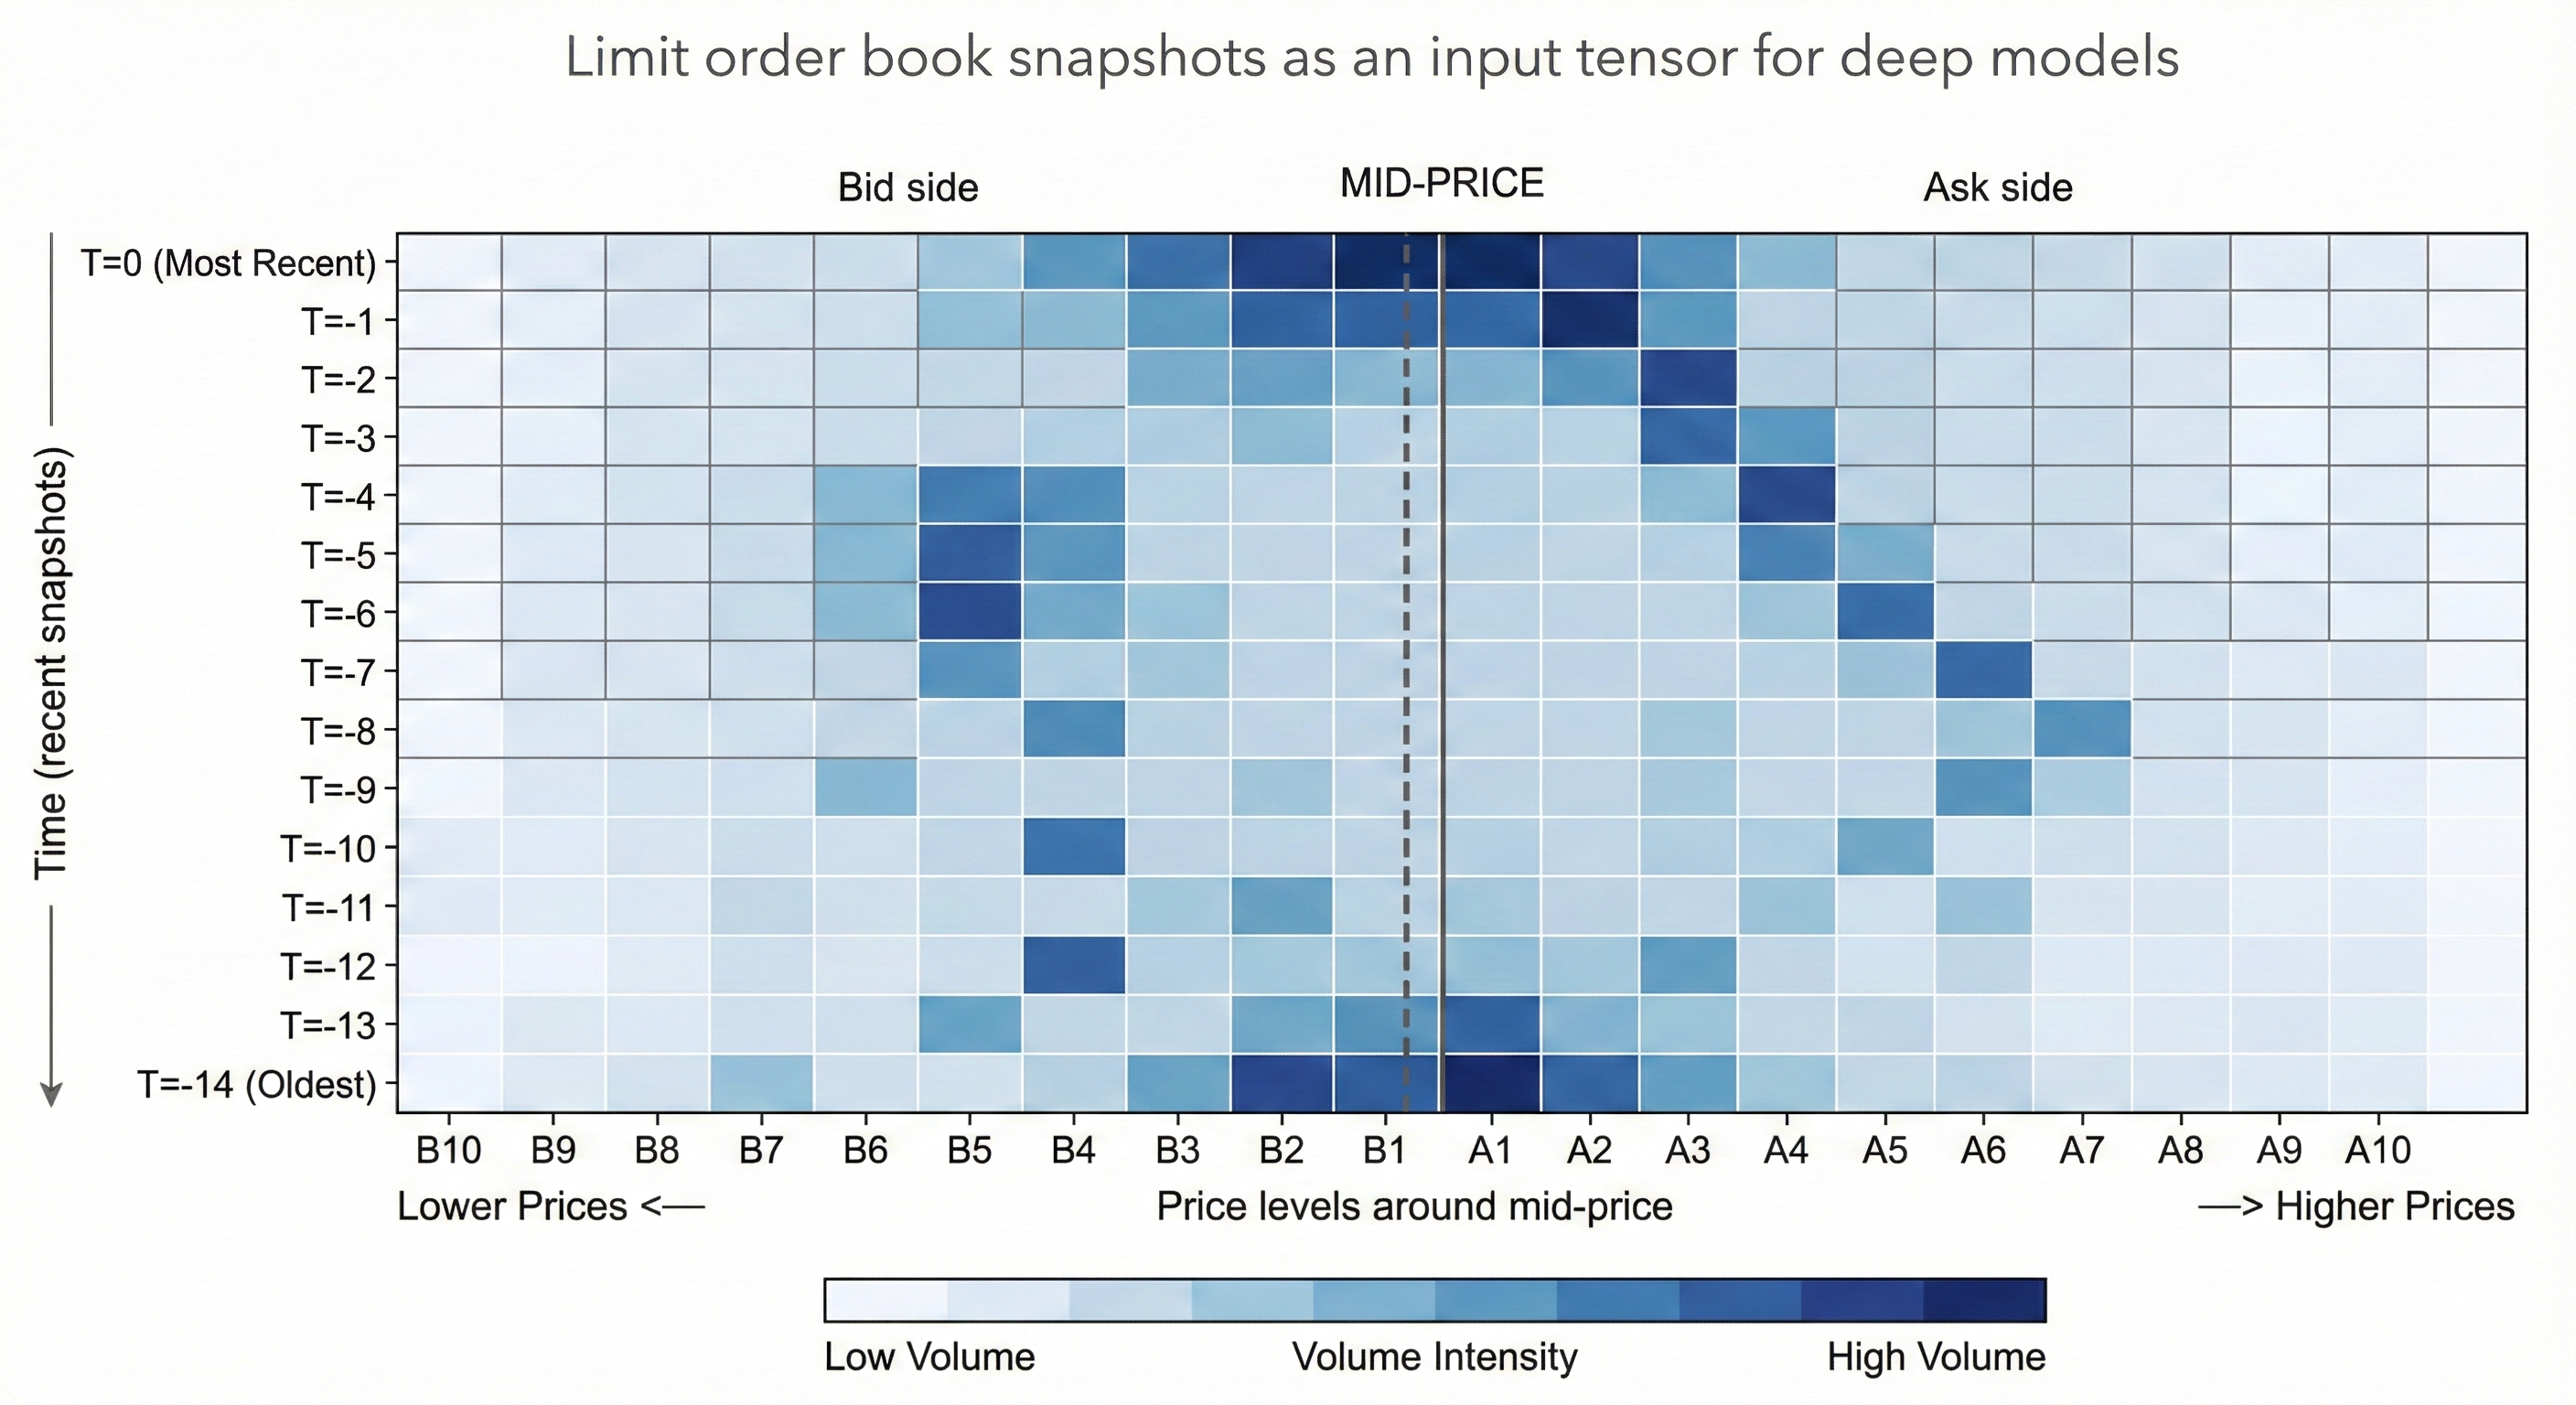
\includegraphics[width=1\textwidth]{imgs/LOB.png}
  \caption[Limit order book input representation.]{\textbf{Limit order book input representation.} Stylised heatmap of bid and ask depths across price levels and time, illustrating the tensor fed to deep LOB prediction models.}
  \label{fig:lob}
\end{figure}

Event-driven models work directly with streams of order-book events (cancellations, limit orders, market orders) containing timestamp, size and price-level information; recurrent, convolutional or attention-based modules summarise these irregular sequences into latent states.

Key microstructure features include realised spread, depth imbalance, bid–ask spread and queue position. Explainability in this setting must therefore connect patterns in prices and volumes to these microstructure concepts, clarifying how the model translates LOB configurations into predicted returns or order-placement decisions.

\subsection{Objectives, Risk and Evaluation}
\label{subsec:trading-objectives}

Unlike credit risk, where models are typically evaluated with classification metrics such as AUROC and calibration, trading models are ultimately judged by their impact on PnL and risk. Given \(\mathrm{PnL}_T\) in~\eqref{eq:trading-pnl}, common evaluation criteria include:
\begin{itemize}
  \item expected return, \(\mathbb{E}[\mathrm{PnL}_T]\), estimated via backtests;
  \item Sharpe ratio, for zero risk-free rate,
  \[
  \mathrm{SR}
  = \frac{\mathbb{E}[\mathrm{PnL}_T]}{\sqrt{\mathrm{Var}(\mathrm{PnL}_T)}},
  \]
  often computed per period;
  \item tail risk, via Value-at-Risk (VaR) or Expected Shortfall (ES) of \(\mathrm{PnL}_T\);
  \item execution quality in optimal execution, measured by implementation shortfall or slippage.
\end{itemize}

\begin{figure}[htbp]
  \centering
  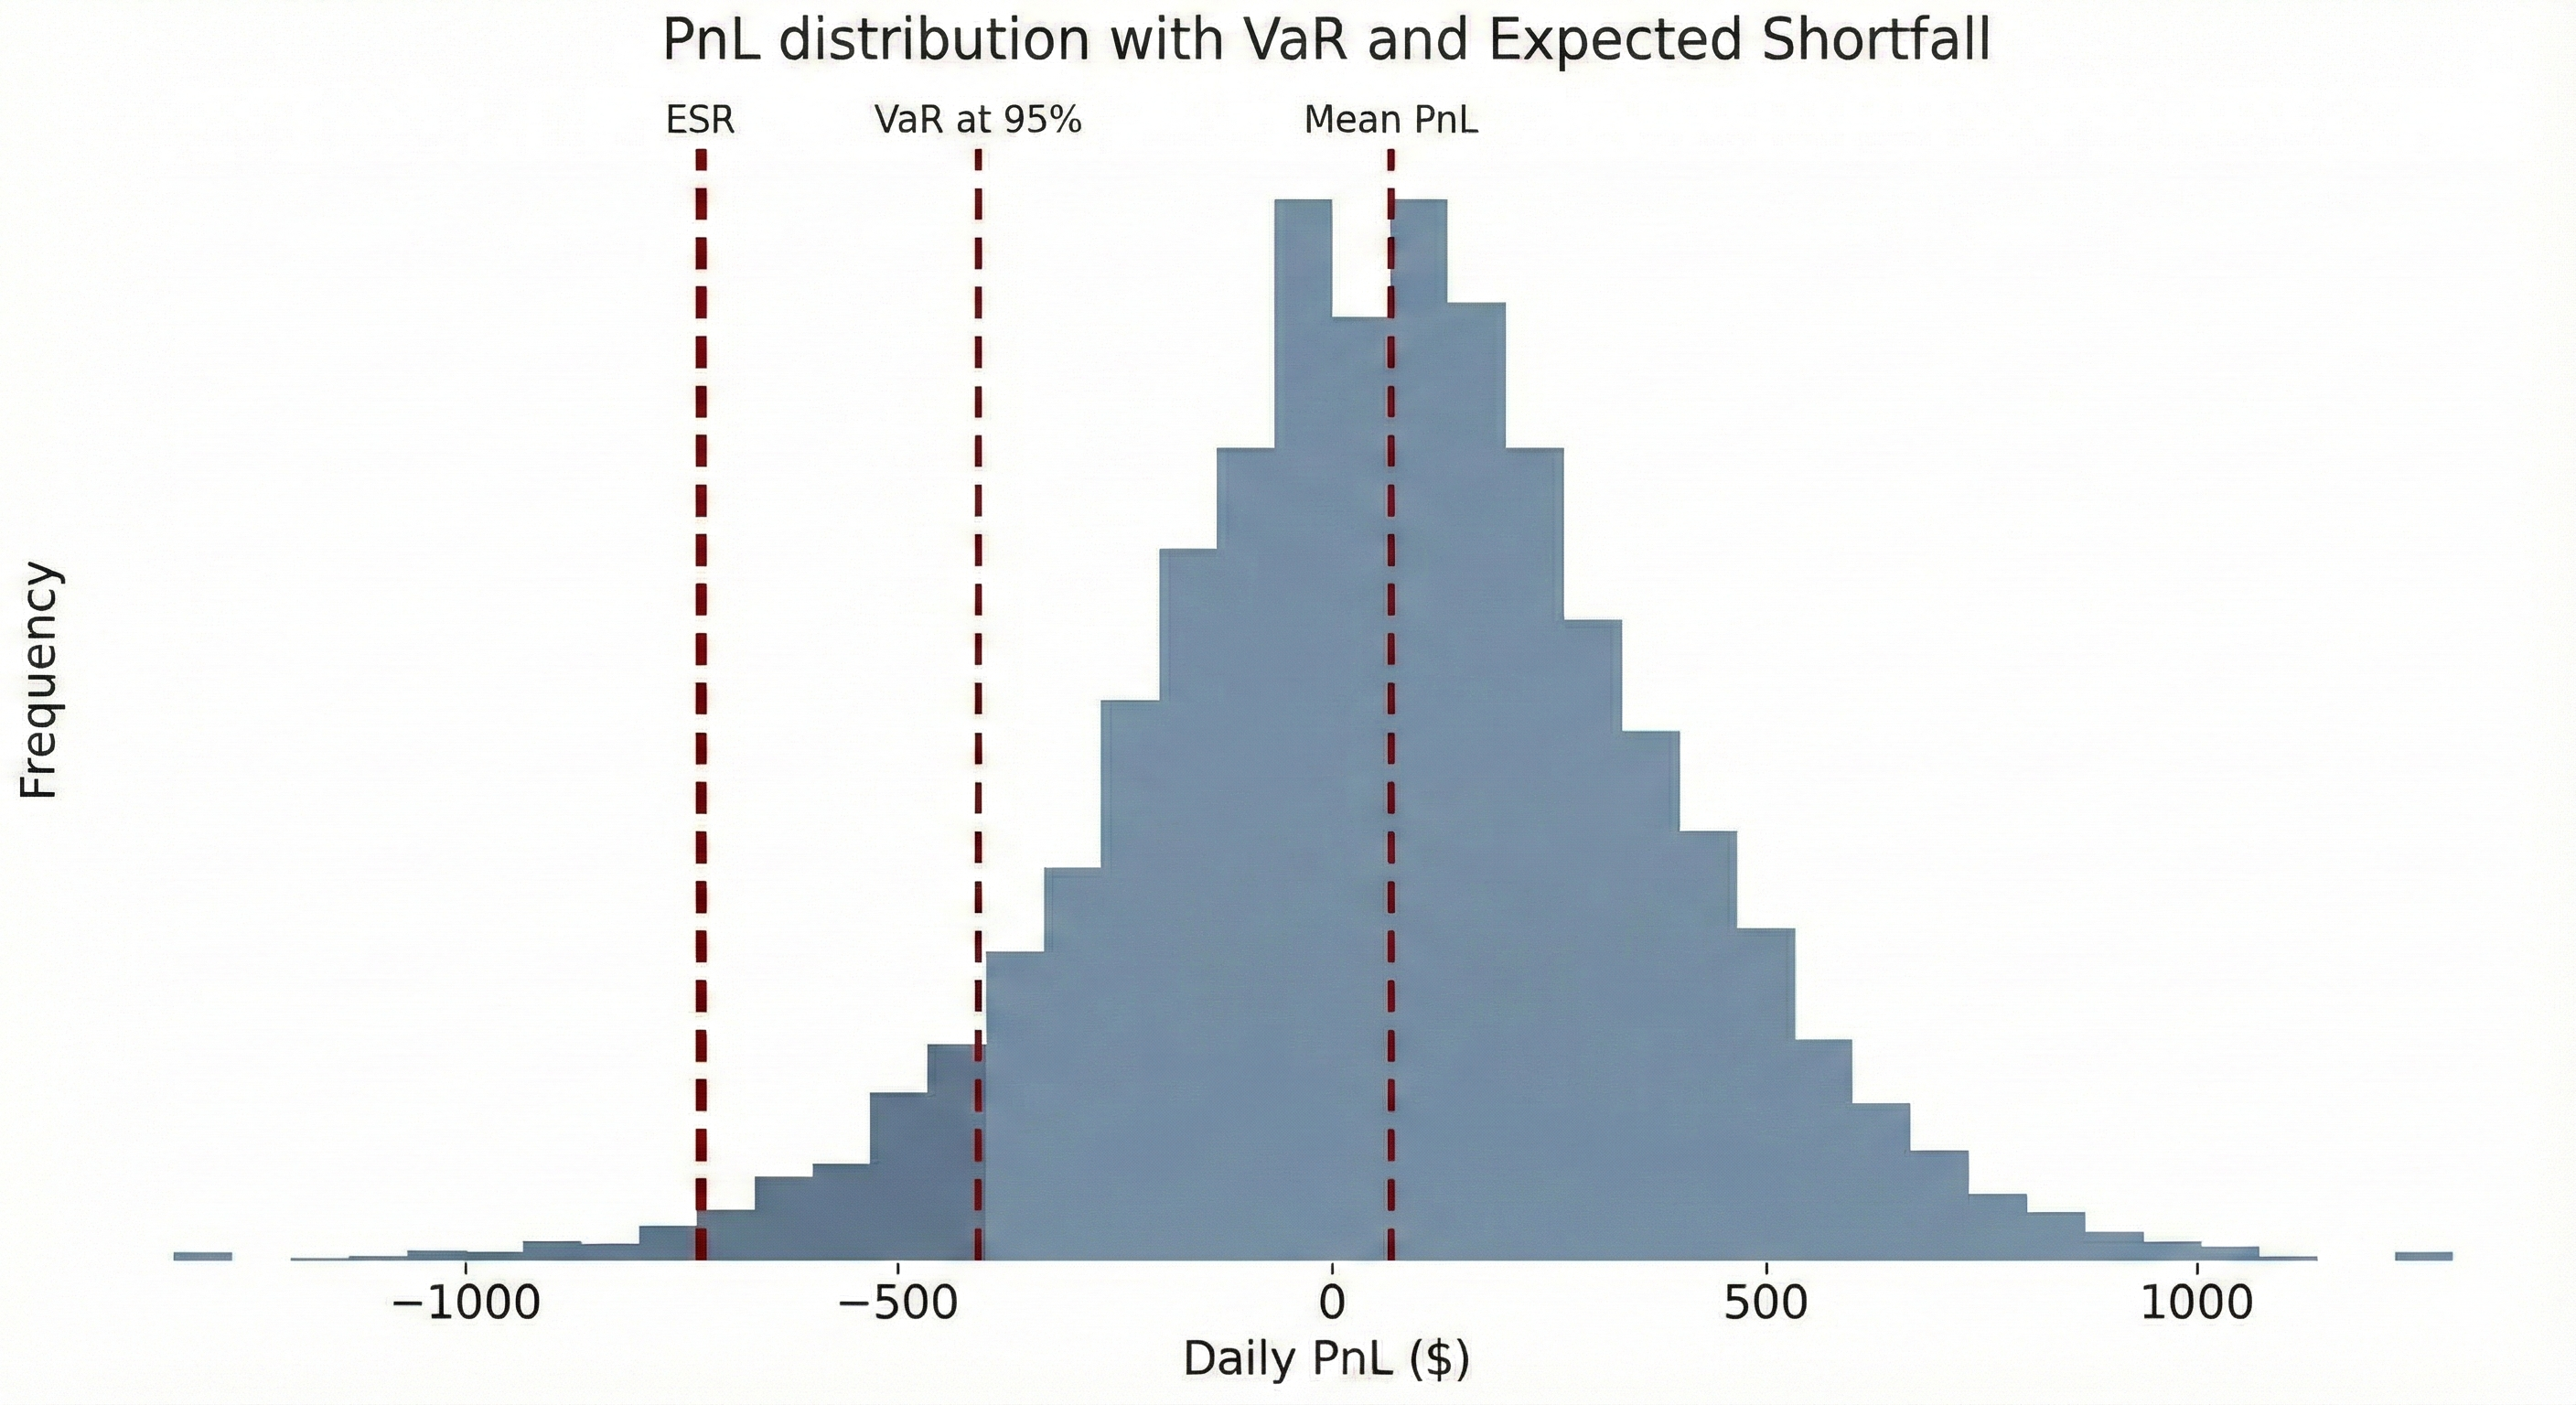
\includegraphics[width=1\textwidth]{imgs/PNL.png}
  \caption[PnL distribution with VaR and ES.]{\textbf{PnL distribution with VaR and ES.} Histogram of daily PnL with lines marking the mean, Value-at-Risk and Expected Shortfall.}
  \label{fig:pnl}
\end{figure}

Models are often trained on surrogate targets (next-step return, directional labels, volatility) but evaluated using portfolio-level PnL metrics that depend on transaction costs, position sizing and capital constraints. A feature that strongly influences forecasts of future returns may not materially affect realised profits once these frictions are taken into account. Explanations must therefore be interpreted both at the level of the predictive model and at the level of the strategy using that model.

\section{AI Models Used}
\label{sec:trading-ai-models}

\subsection{Classical Statistical Models and Tree Ensembles}
\label{subsec:trading-classical}

Before the advent of deep learning, quantitative trading strategies were primarily built around linear and parametric time-series models. For a return series \(\{r_t\}\), ARMA/ARIMA models approximate
\[
r_t
= \mu + \sum_{i=1}^{p} \phi_i\,r_{t-i}
+ \sum_{j=1}^{q} \theta_j\,\varepsilon_{t-j}
+ \varepsilon_t,
\]
with residuals \(\varepsilon_t\) often modelled via GARCH-type conditional volatility processes. Vector autoregressions (VARs) extend this to multivariate systems. Coefficients directly encode lag structures and are intrinsically interpretable.

In cross-sectional equity strategies, linear factor models relate asset returns to economic and style factors,
\[
r_{i,t}
= \alpha_i
+ \sum_{k=1}^{K} \beta_{i,k}\,F_{k,t}
+ \varepsilon_{i,t},
\]
where \(F_{k,t}\) are factors such as market, size, value or momentum. Loadings \(\beta_{i,k}\) and alphas \(\alpha_i\) are interpretable and underpin risk models used in portfolio construction.

Tree ensembles and gradient boosting methods have become standard for both cross-sectional and time-series prediction. Gradient boosting decision trees (GBDT) such as XGBoost or LightGBM use the same additive structure as in Equation~\eqref{eq:gbdt-credit}, but now applied to trading feature vectors \(x_t\) (technical indicators, macro variables, microstructure signals) to produce predicted returns or upward-move probabilities, capturing non-linear interactions in high-dimensional inputs. Empirical studies report that tree-based models can outperform linear baselines on short-horizon prediction tasks, especially when combining technical and fundamental features. As in credit risk, GBDT models are compatible with TreeSHAP, enabling portfolio-level feature attribution analyses that quantify the relative importance of momentum, carry, valuation and microstructure signals.

\subsection{Deep Learning for Time Series and Limit Order Books}
\label{subsec:trading-deep}

Financial time series and LOB data are the focus of many deep learning architectures for financial prediction tasks. In comparison to tree ensembles using hand-crafted features, deep networks can learn representations directly from raw or only lightly processed inputs.

For bar data, Convolutional Neural Networks (CNNs) and Temporal Convolutional Networks (TCNs) treat sequences of OHLCV vectors as multichannel time series; one-dimensional convolutions capture local patterns such as short-term momentum or volatility bursts, and dilation or residual architectures extend the receptive field. Recurrent Neural Networks (RNNs), particularly LSTMs and GRUs, process sequences of returns or indicators to predict future returns or volatility.

For LOB data, specialised architectures such as DeepLOB combine spatial and temporal convolutions with recurrent layers to process sequences of snapshots. A typical pipeline
\[
x_t \in \mathbb{R}^{2K \times L}
\quad\mapsto\quad
\text{CNN} \;\mapsto\; \text{RNN/TCN} \;\mapsto\; \text{classifier}
\]
learns filters over price levels and time, capturing patterns such as steep book slopes, liquidity withdrawal or surges in aggressive orders and outputs classifications of short-horizon mid-price moves.

Transformer architectures have also been proposed for market modelling. Self-attention layers allow the model to relate distant time points without explicit recurrence. Whether a transformer outperforms well-regularised CNN, TCN or LSTM baselines depends on factors such as training data size, signal-to-noise ratio and regularisation choices.

From an XAI perspective, deep models of this type have several characteristics:
\begin{itemize}
\item high-dimensional input (the combination of the dimensions of time and price level and the number of input features);
\item high capacity to fit noise in the training dataset and/or fit artefacts of a specific trading environment;
\item hidden states and/or attention weights generated by the model that may or may not be related to economic concepts.
\end{itemize}

These issues motivate temporal and spatio-temporal tools for explaining models, which are covered in Section~\ref{sec:trading-xai}.

\subsection{Reinforcement Learning and Market Simulation}
\label{subsec:trading-rl}

Reinforcement learning provides a natural framework for trading problems where the decision-maker interacts with the market over time. A standard Markov decision process (MDP) formulation specifies:
\begin{itemize}
  \item state \(s_t\), summarising market and portfolio information (prices, LOB, inventory, realised PnL);
  \item action \(a_t\), specifying orders or target positions;
  \item transition dynamics \(p(s_{t+1}\mid s_t, a_t)\), capturing market evolution and order execution;
  \item reward \(r_t\), typically incremental PnL minus risk or transaction cost penalties.
\end{itemize}

The agent seeks a policy \(\pi(a\mid s)\) maximising expected discounted reward
\[
J(\pi)
= \mathbb{E}\left[\sum_{t=0}^{T-1} \gamma^t r_t\right],
\]
with discount factor \(\gamma \in (0,1]\). Deep RL algorithms parameterise \(\pi\) or value functions \(V^\pi(s)\), \(Q^\pi(s,a)\) with neural networks.

Trading applications of reinforcement learning include optimal execution (reducing implementation shortfall associated with placing a large order), market making (issuing quotes as best bid/best offer while managing inventory and adverse selection risk) and dynamic hedging and asset allocation. Training typically relies on historical replays or generative simulators of market dynamics, so both performance and later explanations depend critically on how well these simulated environments approximate real markets.

Explaining why an agent chooses a particular action from those available in the current state requires an understanding of the agent's value function, the long-term reward structure it uses to guide its actions and the constraints that limit what the agent can do. XAI for RL in trading is therefore less mature than for supervised models; the remainder of this section reviews approaches that provide explanations about why agents act as they do in trading-related RL problems.

\section{XAI Techniques Applied}
\label{sec:trading-xai}

From the perspective of Section~\ref{subsec:terminology}, most XAI methods used in trading are post-hoc: feature attributions for tree ensembles and deep networks, temporal saliency and concept-based explanations for time-series models and surrogate or rule-based approximations for RL policies. This section organises these methods by model class.

\subsection{Feature Attribution for Time-Series Signals}
\label{subsec:trading-feature-attr}

Feature attribution methods (Section~\ref{subsec:feature-attribution}) extend naturally to trading models operating on engineered time-series features. Consider a supervised forecast-and-act model \(f(x_t)\) trained to predict next-period return or price movement based on a feature vector
\[
x_t = (z_{t,1},\dots,z_{t,M}),
\]
where \(z_{t,j}\) are technical or fundamental signals (moving averages, momentum, volatility, valuation, macro surprises).

For tree ensembles, TreeSHAP yields Shapley-based attributions \(\phi_j(x_t)\) for each feature and time \(t\) that satisfy the additive decomposition in Equation~\eqref{eq:fa-additive}; positive \(\phi_j(x_t)\) push the prediction towards higher returns or higher probability of an upward move. Aggregating \(|\phi_j(x_t)|\) over time yields global importance rankings, similar to portfolio-level analyses in credit risk.

For example, suppose a model trades an index using:
\begin{itemize}
  \item \(z_{t,1}\): 5-day momentum;
  \item \(z_{t,2}\): 20-day realised volatility;
  \item \(z_{t,3}\): valuation ratio.
\end{itemize}
For a particular day, TreeSHAP might output
\[
\phi_{\text{mom}}(x_t) = +0.8\%,\quad
\phi_{\text{vol}}(x_t) = -0.3\%,\quad
\phi_{\text{val}}(x_t) = +0.1\%,
\]
relative to a baseline \(\phi_0\), indicating that positive momentum and attractive valuation favour a long position while high volatility penalises it. Aggregated attributions over time reveal whether profitability is driven by economically plausible factors or by fragile artefacts.

For deep time-series models on raw OHLCV sequences, attribution can be computed at the level of input channels and time steps. Given an input tensor \(x \in \mathbb{R}^{L \times C}\) with look-back length \(L\) and channels \(C\), gradient-based methods such as integrated gradients or DeepLIFT compute attributions
\[
\alpha_{t,c} = \text{contribution of channel } c \text{ at lag } t
\]
to the predicted return or class probability. Heatmaps of \(\alpha_{t,c}\) highlight which time steps and variables drove the prediction, for example sustained upward closes and rising volume preceding a long signal. Model-agnostic methods such as KernelSHAP can be applied by grouping input components into interpretable blocks (e.g.\ aggregating time into windows or channels into ``price'' vs.\ ``volume''), reducing dimensionality and making attributions more interpretable.

\subsection{Temporal and Order-Book Explanations}
\label{subsec:trading-temporal}

For LOB models and other spatio-temporal architectures, explanations must respect both time and price dimensions. A LOB-based classifier may take an input tensor
\[
x \in \mathbb{R}^{L \times 2K},
\]
where \(L\) is the number of recent snapshots and \(2K\) corresponds to bid and ask volumes at \(K\) price levels. Deep architectures apply convolutions across time and levels, making direct mapping from outputs to inputs non-trivial.

Gradient-based saliency methods adapted from vision produce saliency maps over the \(L \times 2K\) grid. Given a scalar output \(f(x)\) (for example, the logit of the ``price up'' class), the gradient \(\partial f / \partial x_{t,k}\) quantifies sensitivity to volume at time \(t\), level \(k\). Integrated gradients or SmoothGrad variants mitigate noise and saturation by integrating or averaging gradients along paths between a baseline and the input.

Such saliency maps indicate whether a model reacts to intuitive patterns such as:
\begin{itemize}
\item increased bid-side liquidity close to the best bid;
\item reduced ask-side liquidity at and above the best ask;
\item preceding order-flow imbalances favouring aggressive buying or selling.
\end{itemize}
If saliency concentrates on deep price levels far from the mid-price or on isolated artefacts, this may signal modelling or data problems.

Temporal concept-based explanations generalise this approach to high-level patterns. TCAV-style methods (Section~\ref{subsec:intrinsic-posthoc}) can use labelled sequences representing concepts such as momentum bursts, liquidity droughts or order-flow imbalance shocks to define concept activation vectors in hidden layers. Concept importance scores then measure how strongly the model associates each concept with prediction outcomes or PnL.

For bar-data CNN or TCN models, one-dimensional Grad-CAM variants can be applied: gradients of the output with respect to the feature maps of the last convolutional layer weight those maps, producing temporal importance scores and highlighting subwindows of the look-back horizon that drive forecasts.

\subsection{XAI for Reinforcement-Learning-Based Trading}
\label{subsec:trading-rl-xai}

Explaining RL policies in trading is more complex than explaining supervised forecasts because decisions depend on long-term value and risk encoded in value functions and reward structures.

Consider an agent with value function \(Q_\theta(s,a)\) and policy \(\pi_\theta(a\mid s)\). For a state \(s_t\) and chosen action \(a_t\), explanations should address why \(a_t\) was selected and which state components contributed most to its estimated value.

Feature attribution can be applied directly to \(Q_\theta\) or to an advantage function. For example,
\[
Q_\theta(s_t,a_t)
\approx \phi_0 + \sum_{j=1}^{M} \phi_j(s_t, a_t),
\]
where \(s_t\) is represented by features such as spread, depth, inventory, recent returns and time remaining. Positive \(\phi_j\) indicate features that increase the long-term value of action \(a_t\). In optimal execution, SHAP-style analyses on \(Q_\theta\) can show that tight spreads and high depth contribute positively to aggressive selling, whereas wide spreads and low depth favour passive orders, modulated by time remaining.

Saliency maps over state representations (prices, LOB, inventory trajectories) complement these scalar attributions, indicating which parts of the state the agent attends to when valuing actions. For example, a market-making agent may rely primarily on near-touch levels and inventory when deciding whether to skew quotes.

Surrogate policies provide global rule-based approximations to RL agents. Given logged state–action pairs \(\{(s_t, a_t)\}\), an interpretable surrogate \(\hat{\pi}\) (decision tree or rule list) can be trained to minimise
\[
\hat{\pi}
= \arg\min_{\pi \in \mathcal{G}}\
\frac{1}{N}\sum_{t=1}^{N}\
\ell\bigl(\pi(s_t), a_t\bigr)
+ \Omega(\pi),
\]
where \(\mathcal{G}\) is a class of interpretable policies and \(\ell\) measures disagreement. The resulting rules might read:
\begin{quote}
If spread is small, bid-side depth is high and inventory is below target, then place a buy limit order at the best bid; otherwise, hold.
\end{quote}
Fidelity is evaluated by agreement between \(\hat{\pi}(s_t)\) and the original policy and by comparing PnL and risk distributions in simulation.

Analysing how explanations change as reward weights on inventory or transaction costs vary in
\[
r_t = \Delta \mathrm{PnL}_t
      - \lambda_\mathrm{inv} \, \mathrm{InvRisk}_t
      - \lambda_\mathrm{tc} \, \mathrm{Tcost}_t
\]
clarifies trade-offs encoded in the reward function (for example, how much profit the agent is willing to sacrifice to control inventory). However, such analyses remain largely qualitative and rely heavily on the fidelity of the training environment.

\subsection{Global Surrogates and Rule-Based Strategy Summaries}
\label{subsec:trading-surrogates}

Beyond local explanations, practitioners often require global summaries that describe how a strategy behaves across markets and regimes. As in credit risk (Section~\ref{subsubsec:surrogates-formulation}), surrogate models and rule lists can approximate complex predictors and policies with more interpretable forms.

In a forecast-and-act setting, an interpretable surrogate \(g : \mathcal{X} \to \mathbb{R}\) can be fitted for the signal \(f(x_t)\), or a surrogate policy \(\hat{\pi} : \mathcal{X} \to \mathcal{A}\) can be learnt for the induced actions \(a_t\). For a gradient boosting model mapping features \(x_t\) to a predicted return \(f(x_t)\) and a trading rule converting this into \(a_t \in \{-1,0,+1\}\), a depth-limited decision tree surrogate \(\hat{\pi}\) can be trained as
\begin{equation}
  \label{eq:rl-surrogate-policy}
  \hat{\pi}
  = \arg\min_{\pi \in \mathcal{G}}
    \frac{1}{N} \sum_{t=1}^{N}
      \ell\bigl(\pi(x_t), a_t\bigr)
    + \Omega(\pi),
\end{equation}
where \(\mathcal{G}\) restricts depth and number of leaves. The resulting tree might implement rules such as:
\begin{quote}
If 10-day momentum is positive, short-term volatility is low and spread is tight, then go long;\\
else if 10-day momentum is negative and order-flow imbalance is negative, then go short;\\
otherwise, stay flat.
\end{quote}

For RL policies, an analogous distillation procedure yields compact rule lists summarising execution or market-making heuristics, such as:
\begin{quote}
If remaining time \(>\) 30\% of the horizon and spread \(<\) 2 ticks, then trade aggressively;\\
else if inventory is large and volatility is high, then slice orders more finely;\\
else trade passively at the best bid/ask.
\end{quote}
These rules are easier to audit and to compare with existing policies and limits \cite{XAiTimeSeriesForecasting2024,XAiFinanceReview2025}. Fidelity metrics (agreement rates, PnL and risk differences) indicate how far the surrogate can be trusted as a description of the underlying strategy.

Overall, XAI for RL-based trading is less mature than for supervised models. Value-function feature attributions and state saliency provide local insight into which variables (depth, spread, inventory, time) matter for decisions, while surrogate policies summarise high-level behaviour. Explaining exploration–exploitation trade-offs, long-horizon risk management and sensitivity to environment assumptions remains considerably more difficult than explaining single-step predictions.

\section{Strengths, Limitations and Open Issues in Trading}
\label{sec:trading-limitations}

\subsection{Strengths and Practical Benefits}
\label{subsec:trading-strengths}

Throughout the trading lifecycle, XAI supports qualitative validation, risk control and internal communication. The main strengths can be summarised as:
\begin{itemize}
  \item \emph{Economic sanity checks for signals.}
  Feature attribution and temporal saliency help determine whether a model relies on economically meaningful drivers (momentum, carry, volatility, liquidity) or artefacts (calendar quirks, isolated queue levels). SHAP analyses can show that profitability is driven by well-established factors with limited contribution from opaque residual features, or flag spurious dependencies for further investigation.

  \item \emph{Regime-aware diagnostics.}
  Comparing attributions across bull, bear and crisis periods reveals how model behaviour changes with market regimes. For example, temporal explanations can show reduced reliance on trend signals and increased weight on volatility or mean-reversion indicators during turbulent markets, helping assess qualitative robustness.

  \item \emph{Communication between research, portfolio management and risk.}
  Explanations expressed in terms of trend, volatility, liquidity and valuation provide a common language for quantitative researchers, portfolio managers and risk controllers. This facilitates discussions of strategy logic, conditions for profitability and potential failure modes in investment committees and risk forums.

  \item \emph{Scenario analysis and stress testing.}
  Combining scenario-based market paths with feature attributions shows which signals drive decisions under stress, how positions concentrate and how changes in liquidity or volatility affect strategy behaviour. Surrogate models with monotonic or structural constraints offer simplified approximations suitable for aggregated risk analysis.

  \item \emph{Design and monitoring of RL agents.}
  For RL-based strategies, explanations of value functions and surrogate policies clarify how agents trade off profit against inventory and transaction costs. These insights support reward shaping, position-limit design and detection of pathologies (e.g.\ exploiting simulator artefacts or taking excessive tail risk).
\end{itemize}

\subsection{Limitations of XAI Techniques in Algorithmic Trading and Market Forecasting}
\label{subsec:trading-failure-modes}

The benefits above are constrained by several domain-specific limitations:
\begin{itemize}
  \item \emph{Non-stationarity and regime shifts.}
  Explanations based on historical data describe behaviour in past regimes but may fail in future regimes if market structure or competitor behaviour changes, or if the strategy itself influences prices. Explanations are therefore descriptive rather than predictive for future performance.

  \item \emph{Noise and label instability.}
  Short-horizon returns are extremely noisy, so labels such as ``up'' or ``down'' over a few seconds or minutes are unstable. Models and XAI techniques can both fit and explain patterns that largely reflect noise. This creates a risk of ``explanation overfitting'', where explanations appear plausible but merely re-describe random fluctuations.

  \item \emph{Overfitting and backtest selection bias.}
  Repeated backtesting on the same dataset encourages selection of strategies that fit historical noise. XAI can exacerbate this if researchers favour models whose explanations match pre-existing market narratives. The strategy that looks profitable and has intuitive explanations may simply be the lucky one; out-of-sample and out-of-time validation of both performance and explanations is required.

  \item \emph{Causality, reflexivity and proxy effects.}
  As in credit risk, feature attributions measure predictive usage, not causal effects. Financial variables are correlated, and some signals may act as proxies for hidden liquidity, market structure or other participants’ behaviour. Reflexivity further complicates causal interpretation: trading on an identified pattern can alter or destroy it, so explanations cannot be treated as causal guarantees.

  \item \emph{Adversarial and strategic constraints.}
  Trading is adversarial. Detailed explanations of proprietary strategies risk revealing alpha and enabling front-running or reverse engineering. In practice, firms limit detailed XAI analyses to internal audiences and focus external communication on aggregate risk and control views, which constrains how far XAI can be used for external transparency.

  \item \emph{Dependence on RL environments.}
  For RL-based systems, explanations grounded in value functions or surrogate policies are only as reliable as the simulators used for training. If simulators omit important dynamics (hidden liquidity, latency, other traders’ adaptation), explanations may accurately describe behaviour in simulation but be misleading for live markets.

  \item \emph{Computational cost and incomplete tooling.}
  Computing SHAP values or integrated gradients for large time-series or LOB datasets is computationally expensive, especially for multiple models and frequent retraining. Tooling for XAI in trading is less standardised than in credit risk, limiting how systematically explanations are generated and monitored in production.
\end{itemize}

\subsection{Open Issues and Research Directions}
\label{subsec:trading-open-issues}

Several open issues characterise the current state of XAI in algorithmic trading and market forecasting:
\begin{itemize}
  \item \emph{Evaluation frameworks for non-stationary environments.}
  Most explanation-quality metrics (local fidelity, stability, sparsity) assume static tasks. In trading, evaluation must incorporate regime shifts and adaptive strategies. One direction is to track how explanation patterns evolve relative to performance and to test whether changes in explanations provide early warning signals for strategy degradation.

  \item \emph{Joint design of models and explanations under market constraints.}
  As in credit risk, models and explanations are typically designed independently. A promising line of work constrains models to satisfy trading-specific explainability requirements, such as monotonic dependence on key risk factors, sparse reliance on microstructure features or decompositions into interpretable modules (signal, risk control, execution). Regularising for stable and economically meaningful explanations, while maintaining performance, may reduce explanation overfitting.

  \item \emph{Temporal and structural concept discovery.}
  Temporal concept-based explanations remain underdeveloped. Methods that discover and validate concepts such as ``momentum burst'', ``liquidity drought'' or ``order-flow imbalance shock'' within deep representations could bridge learned features and trader intuition. This requires combining unsupervised representation learning, concept activation and economic labelling.

  \item \emph{Explainability for multi-asset portfolios and constraints.}
  Many strategies operate at portfolio level, coordinating decisions across assets under risk and capital constraints. Explaining such systems requires attributing not only individual signals per asset but also cross-asset interactions, diversification effects and binding constraints (sector caps, leverage limits). Extending XAI techniques to portfolio optimisation and portfolio-level risk management is an important research direction.

  \item \emph{Integration of XAI into governance and oversight.}
  Integration of XAI into trading-strategy governance is currently ad hoc. Open questions include when explanations must be generated (model approval, periodic review, post-drawdown), how they should be documented and stored, and how they should influence decisions on capital allocation, limits and model retirement. Compared with credit risk, governance structures must balance internal risk management needs with the proprietary nature of trading strategies.
\end{itemize}

% =========================
% Chapter 4: Cross-Domain Comparison and Synthesis
% =========================
\chapter{Cross-Domain Comparison and Synthesis}
\label{chap:comparison}

In this chapter, we combine the findings from credit risk (Chapter~\ref{chap:credit-risk}) and trading (Chapter~\ref{chap:trading}) to address the central research question: What does XAI really bring to financial decision-making when using flexible models, and how does that vary per domain?

\section{Axes of Comparison}
\label{sec:comparison-axes}

The two domains differ along several structural dimensions:

\begin{itemize}
  \item \textbf{Data and targets.} Credit risk uses static or slowly changing tabular borrower data and binary default events; trading uses high-frequency time series and LOB states, with objectives defined on returns and PnL.
  \item \textbf{Constraints and incentives.} Credit models operate under strong regulatory, fairness and consumer-protection constraints. Trading models are primarily governed by risk limits, market impact and internal governance.
  \item \textbf{Model classes.} Most credit risk models use logistic regression and gradient-boosting trees, with some applications of deep networks. Trading uses a greater variety of models, including tree ensembles, deep sequence models and reinforcement-learning agents.
  \item \textbf{Explanatory needs.} Explanations for credit risk need to be sufficient to justify adverse action notices, to support supervisory review and to support internal model risk management. Explanations for trading need to support strategy development, debugging and communication between quantitative teams, portfolio managers and risk teams.
\end{itemize}

These differences shape which XAI methods are used and how their strengths and weaknesses manifest.

\section{Patterns Across Credit Risk and Trading}
\label{sec:comparison-patterns}

Across both domains, researchers and practitioners observe similar patterns in how feature explanation and attribution techniques are applied to different types of machine learning models.

First, since tree-ensemble models are so prevalent, feature attribution techniques based on Shapley values (such as SHAP and TreeSHAP) are the default choice for producing additive decompositions of model predictions with guaranteed theoretical properties at an acceptable cost. These techniques are already used in production settings in the credit risk domain to produce reason codes for loan decisions and are used by traders as diagnostic tools for validating the behaviour of multi-signal models.

Second, counterfactual explanations are essentially a credit-risk tool. Given that they focus on individualised recourse and require minimal changes to covariates, these types of explanations are best suited for use in consumer lending applications where fairness and regulatory compliance are key. In the trading domain, there is no equivalent of a “borrower” attempting to improve features; when evaluating alternative courses of action, practitioners typically modify or replace strategies rather than changing exogenous covariates. Portfolio-level scenario analysis and stress testing are therefore better suited than pointwise counterfactual explanations.

Third, surrogate models and rule-based explanations occupy specific niches within each domain. In credit risk, shallow trees and rule lists are often used to approximate the behaviour of more complex gradient boosting models, helping to bridge the gap between these models and more traditional scorecard-based approaches. In the trading domain, surrogates are most commonly used to check whether a model behaves reasonably or to explain the behaviour of a reinforcement-learning policy to human stakeholders. In both domains, the fidelity–interpretability trade-off is critical: if a surrogate model is too simple, it may fail to capture the complexities of the decision boundary of the original model; conversely, if a surrogate model is too complex, it will likely lose most of its interpretability.

Fourth, deep learning has increased both the need for explainable AI (XAI) and the fragility of existing XAI tools. While tree ensembles with SHAP provide a relatively stable pipeline for explaining tabular credit models, for the sequence and LOB models used in the trading domain, XAI remains largely exploratory. Gradient-based saliency and concept-based methods do provide some insight into the operation of deep models; however, the stability of these methods, as well as their economic interpretation, is much less well documented than for their tabular counterparts, and the conclusions drawn from them are sensitive to factors such as the structure of the data, the model architecture and the regime in which the model is operating. This is also true for reinforcement learning (RL): researchers are developing prototype explanations of policies and value functions, but these remain mostly research tools and are not yet standard model-risk tools.

Finally, both domains highlight the distinction between predictive and causal explanations. In credit risk, feature attribution methods and counterfactual explanations can provide some guidance on what features a borrower can realistically change. At the same time, they can create unrealistic expectations about the degree to which borrowers can influence their creditworthiness. Similarly, in the trading domain, feature attributions can create unrealistic expectations about the reliability of patterns that are in fact transitory or regime-specific. In neither domain does current XAI practice provide a causal understanding of why the model made the prediction; rather, it provides a structured summary of how the model behaved given the observed data distribution.

\begin{figure}[htbp]
  \centering
  \includegraphics[width=1\textwidth]{imgs/Comparison.png}
  \caption[Qualitative Comparison of XAI Methods.]{\textbf{Qualitative Comparison of XAI Methods.}}
  \label{fig:comparison}
\end{figure}

% =========================
% Chapter 5: Conclusion
% =========================
\chapter{Conclusion}
\label{chap:conclusion}

This dissertation examined how explainable artificial intelligence (XAI) could act as a mediator between the predictive capacity of the large-scale machine learning (ML) models used in financial applications and the need for transparency required in financial decision-making.

To accomplish this investigation, this thesis focused on the fields of credit risk assessment and algorithmic trading, and analyzed the types of ML models currently being employed in each field, the types of XAI techniques being applied to them, and the success and/or failures of those XAI techniques based on factors including fidelity, stability, interpretability, actionability, fairness, and computational cost.

It was found through the research in the field of credit risk that Gradient Boosted Decision Trees (GBDTs), combined with Shapley value-based feature attribution (also known as SHAP), had developed to the point of maturity that they could meet the transparency requirements necessary for their use within regulated environments.

TreeSHAP explanations enable institutions to employ GBDT models that perform better than logistic regression, and at the same time, provide auditable reasons for why decisions were made, as well as portfolio-wide views of what drives risk.

Counterfactual explanations and surrogate rule-based models expand upon this toolset, by enabling institutions to provide recourse-based explanations, and global summaries of model behaviour, however, this toolset has a number of significant caveats regarding its feasibility, fairness, background choice, and the fact that attributions are non-causal.

In the area of trading, XAI is less standardized, however, it is rapidly becoming a diagnostic layer atop tree ensembles, deep time series architectures, and reinforcement learning-based strategies.

Feature attribution, temporal saliency maps, and concept-based analyses assist in connecting complex models to economic and microstructure concepts; surrogate policies and value function attributions assist in partially understanding RL agent behaviour.

However, the nonstationarity of the environment, the indirect relationship between point-wise predictive accuracy and realized PnL, and lower levels of external regulatory pressure limit the extent to which such explanations may be considered stable guarantees, versus context-specific analyses.

Ultimately, XAI emerged in this research not as a solution to the opacity of modern AI, but as an organized collection of tools that, if used thoughtfully, can augment model governance.

Its primary strengths include the ability to make model behaviour observable, to surface unforeseen dependencies, and to provide a common language for dialogue between quantitative teams, domain experts, and oversight bodies.

Its primary weaknesses include the separation between statistical associations and causal mechanisms, the dependency of explanations on modeling and background choices, and the potential for visually appealing explanations to foster confidence in models whose fragility has been previously demonstrated.

Several paths for future research were identified in this dissertation. First, there is a need for standards and benchmarks for evaluating the quality of explanations in finance, including quantitative measures of stability, fairness-aware analyses, and human-in-the-loop evaluations that connect explanations to actual decision quality.

Second, jointly developing models and explanation mechanisms -- using constraint architectures, explanation-aware regularization, and causal structure -- provides a route toward bridging the gap between intrinsic and post-hoc interpretability in both credit and trading.

Third, extending XAI to dynamic, multi-modal financial environments, where sequential data, text, and network structures interact, will necessitate explanation tools that operate cohesively across horizons, instruments, and decision makers.

Under these conditions, the conclusions drawn in this dissertation support a cautiously optimistic view: with sufficient safeguards, XAI enables financial institutions to capitalize on the predictive capabilities of modern AI while maintaining some measure of transparency and control.

The objective is not to eradicate opacity completely; instead, the aim should be to ensure that complexity is utilized wherever it offers added value, and that explanation methods are similarly evaluated and governed rigorously.
\label{sec:final-remarks}

% Bibliography
\bibliographystyle{plain}
\bibliography{references}

\end{document}
